%%%%%%%%%%%%%%%%%%%%%%%%%%%%%%%%%%%%%%%%%%%%%%%%%%%%%%%%%%%
% Main thesis file
% Goal: provide structure for my MSc thesis
% Authors: Mathias Payer <mathias.payer@epfl.ch>, Gaiëtan Renault <gaietan.renault@alumni.epfl.ch>
%
% This work may be distributed and/or modified under the
% conditions of the LaTeX Project Public License, either version 1.3
% of this license or (at your option) any later version.
% The latest version of this license is in
%   http://www.latex-project.org/lppl.txt
%
%%%%%%%%%%%%%%%%%%%%%%%%%%%%%%%%%%%%%%%%%%%%%%%%%%%%%%%%%%%
\documentclass[a4paper,11pt,oneside]{report}

\usepackage[MScThesis,lablogo]{packages/EPFLreport} % Options: MScThesis, BScThesis, MScProject, BScProject, % NOTE: Modified by G. Renault
\usepackage{xspace}
\usepackage{indentfirst} % Added by G. Renault
\usepackage{float} % Added by G. Renault
\usepackage{svg}   % Added by G. Renault
\usepackage[ruled,vlined, linesnumbered]{algorithm2e} % Added by G. Renault
\usepackage{amsfonts} % Added by G. Renault
\raggedbottom % Added by G. Renault
\setlength {\marginparwidth }{2cm}
\usepackage[disable]{todonotes} %disables all todonotes
\newcommand{\ali}[1]{\todo[inline,color=red!40]{alice: #1}} % inline comment block
\usepackage{cleveref} % Added by G. Renault

\title{NinjaCrane: a Cybersecurity Attack Demonstrator on a Polar Crane's Industrial Control System (ICS)}
\author{Gaiëtan Renault}
\supervisor{Nicolas Sursin}
\adviser{Prof. Dr. sc. ETH Mathias Payer}
%\coadviser{Second Adviser} % TODO
\expert{Nicolas Sursin} % TODOs

\begin{document}
\maketitle
\makededication
\makeacks


\input{}

\begin{abstract}
Despite the sophisticated \emph{Stuxnet} attack discovered in 2010, the cybersecurity awareness around the \emph{Industrial and Control System} (ICS) remains a challenge~\cite{Pattanayak18}. The necessity to train ICS actors and to raise awareness on this issue increases~\cite{Wang22}~\cite{wong22}~\cite{cisaTraining}. Moreover, listing the cybersecurity best practices to follow regarding a security policy has a limited impact on their effectiveness compared to an awareness program~\cite{Rhee09}~\cite{Sitnikova13}~\cite{Angafor20}. In this context, this Master’s Project builds a cyberattack demonstrator targeting a part of a nuclear power-plant ICS and more precisely a polar crane's \emph{control system}. The described attack, called \emph{NinjaCrane}, infects an engineering workstation through an USB cable or a maliciously tampered mouse and deploys a malware targeting the communication with a \emph{Modicon M580}, a \emph{Programmable Logic Controller} (PLC), by conducting a \emph{Meet-In-The-Middle Attack} (MITM) exploiting the CVE-2022-45789 (Capture-replay attack) and the CVE-2021-22779 vulnerability (a.k.a. \emph{ModiPwn}). This work illustrates and highlights the necessity to respect the ICS security policy and may well suit an awareness program.

\iffalse
The \sysname tool enables lateral decomposition of a multi-dimensional flux compensator along the timing and space axes.

The abstract serves as an executive summary of your project.
Your abstract should cover at least the following topics, 1-2 sentences for each: what area you are in, the problem you focus on, why existing work is insufficient, what the high-level intuition of your work is, maybe a neat design or implementation decision, and key results of your evaluation.
\fi
\end{abstract}

\begin{frenchabstract}
Malgré la sophistication de l'attaque \emph{Stuxnet}, découverte en 2010, la prise de conscience sur l'importance de la cybersecurité des systèmes de supervision reste encore en marge~\cite{Pattanayak18} et la necessité de former les acteurs industriels sur cette problématique apparaît comme croissante~\cite{Wang22}~\cite{wong22}~\cite{cisaTraining}. De plus, lister les bonnes pratiques vis-à-vis d'une politique de sécurité peut avoir un impact limité sur leur réussite en comparaison à une démarche de sensibilisation~\cite{Rhee09}~\cite{Sitnikova13}~\cite{Angafor20}. Dans ce cadre, ce Projet de Master vise à construire un démonstrateur d'attaque visant une partie d'un système industriel de contrôle d'une centrale nucléaire et plus précisément le \emph{Contrôle-Commande} (CC) du pont polaire. L'attaque présentée ici, appelée \emph{NinjaCrane}, infecte une station d'ingénierie grâce à un câble USB infecté ou une souris modifiée et déploie un logiciel malveillant visant la communication avec le \emph{Modicon M580}, un \emph{Automate Prgorammable Industriel} (API), en conduisant une attaque de type \emph{Homme Du Milieu} (HDM) exploitant les failles CVE-2022-45789 (une attaque par rejeu) et CVE-2021-22779 (appelée \emph{ModiPwn}). Ce travail illustre et souligne la necessité du respect de la politique de sécurité et s'inscrit dans une démarche de sensibilisation.

\iffalse
For a doctoral thesis, you have to provide a French translation of the
English abstract. For other projects this is optional.
\fi
\end{frenchabstract}

\cleardoublepage
%%%%%%%%%%%%%%%%
% Notation
%%%%%%%%%%%%%%%%
\begin{notation}
\section*{List of Acronyms}
\vspace{0.5cm}
\begin{center}
    \begin{tabular}{c@{\hskip 1in}l} 
        \hline
        Abbreviations & Meaning \\
        \hline
        APT & Advanced Persistent Threat \\
        ARP & Address Resolution Protocol \\
        BLE & Bluetooth Low Energy \\
        CB & Reactor Containment Building or Reactor Building \\
        CISA & Cybersecurity and Infrastructure Security Agency \\
        DCS & Distributed Control System \\
        DMZ & DeMilitarized Zone  \\
        DOE & Department of Energy \\
        EDF & Électricité de France \\
        FBI & Federal Bureau of Investigation \\
        GRFICS & Graphical Realism Framework for Industrial Control Simulations \\
        HID & Human Interface Device \\
        HMI & Human Machine Interface \\
        ICS & Industrial Control System \\
        IIoT & Industrial Internet of Things \\
        IS & Information System \\
        IT & Information Technology \\
        MITM & Meet-In-The-Middle \\
        MSc & Master of Science \\
        NPP & Nuclear Power Plant \\
        NSA & National Security Agency \\
        OPSWAT & Omni-Platform Security with Access Technologies \\
        OT & Operational Technology \\
        PLC & Programmable Logic Controller \\
        RS232 & Recommended Standard 232 \\
        RTU & Remote Terminal Unit \\
        SCADA & Supervisory Control And Data Acquisition \\
        TTL & Transistor-Transistor Logic (serial communication) \\
        UAC & User Account Control \\
        UMAS & Unified Messaging Application Services \\
        USB & Universal Serial Bus \\
        VM & Virtual Machine \\
        [1ex] 
        \hline
        \rule{0pt}{10ex}
    \end{tabular}
\end{center}

\cleardoublepage

\section*{List of Notation}
\vspace{0.5cm}
\begin{center}
    \begin{tabular}{c@{\hskip 1in}p{10cm} @{}} 
        \hline
        Notation & Meaning \\
        \hline
        $x_{\textrm{(utf-16-le)}}$ & UTF-16 little-endian encoded string\\
        $x_{\textrm{(base64)}}$ & Base64 encoded string \\ 
        \texttt{SHA256($x$)} & Secure Hash Algorithm 2 with a 256-bits digest of the input $x$ \\
        $\mathbb{N}$ & Natural numbers set \\
        $(x \bmod{y})$ &  Signed remainder of the division of $x$ by $y$ \\
        $\{0, ..., x\}$ &  Set containing all the integers from $0$ (included) to $x$ (included) \\
        $x \gets x_{0},...,x_{n}$ & $x$ is a string made of the ordered concatenation of the characters $x_{0}$ up to $x_{n}$ \\
        $s_1 + s_2$ & Concatenation of the strings $s_1$ and $s_2$\\
        \texttt{0xXX} & Hexadecimal representation of \texttt{XX} (e.g., \texttt{0xA5} is equal to $165$)\\
        [1ex] 
        \hline
    \end{tabular}
\end{center}
\end{notation}
\maketoc
%%%%%%%%%%%%%%%%%%%%%%
\chapter{Introduction}
% This section is usually 3-5 pages.
%%%%%%%%%%%%%%%%%%%%%%

% The introduction is a longer writeup that gently eases the reader into your thesis~\cite{dinesh20oakland}. Use the first paragraph to discuss the setting.
The notorious \emph{Stuxnet} attack~\cite{LangnerStuxnet},~\cite{SymantecStuxnet} the first \emph{Advanced-Persistent Threat} (APT) that subverted an \emph{Industrial and Control System} (ICS), spurred cybersecurity research on this domain. Since then, we observe increasing threats in the ICS domain as show the recent and major attacks, e.g., \emph{Colonial Pipeline}, \emph{CaddyWiper}, \emph{Industroyer2} etc. Moreover, the energy sector is a \emph{Critical Infrastructure} (CI) sector which makes it a target of particular interest~\cite{cisaCI}. Indeed, the \emph{Kaspersky Lab} lists, as a half-year report, the most noticeable attacks in ICS and claims that in the energy sector in 2022 about 34.5\% of the ICS computers (in \emph{Kaspersky Security Network}) have blocked malicious objects~\cite{KasperskyReport}. However, cybersecurity in the energy sector still needs to be developed — in April 2022, the joint cybersecurity advisory ``urge[d] critical infrastructure organizations, especially energy sector organizations, to implement detection and mitigation mechanisms and harden their ICS/SCADA devices`` — DOE, CISA, NSA, and FBI ~\cite{CSA22}. In this context of enhancing cybersecurity in ICS, this work, as part of a Master's Project in industry at \emph{Electricité de France} (EDF), builds a demonstrator attack called \emph{NinjaCrane} on a part of an ICS representative of what can be found in a Nuclear Power Plant (NPP) station. \emph{NinjaCrane} is a practical ICS cyberattack which raises awareness on the importance to respect the cybersecurity policies. The targeted ICS is a polar crane's control system, where the polar crane is a standalone equipment introducing and handling components within the reactor containment building. 

% In the second paragraph you can introduce the main challenge that you see.

Compared to the \emph{Information Technology} (IT) cybersecurity~\cite{nistIT}, the \emph{Operational Technology} (OT) cybersecurity is relatively new~\cite{nistOT}. OT cybersecurity is a change of paradigm where priority is given to availability followed by integrity to achieve one goal — safety. The following typical characteristics and challenges can be noted in an OT environment; low powered hardware with small cybersecurity capabilities and low cybersecurity monitoring, presence of custom closed-source solutions due to the importance of patents in the industry, safety comes before cybersecurity, complexity to update the system as it can stop the industrial process and as any modification needs to be qualified, presence of 3rd-party solutions, and finally still a relatively low awareness on the cybersecurity policy despite the fact that the human is generally a key asset directly interacting with the ICS.

% The third paragraph lists why related work is insufficient.
To cite similar works that have been done to illustrate an industrial cyberattack, the \emph{Graphical Realism Framework for Industrial Control Simulations} (GRFICS) models a destructive attack on the simplified \emph{Tennessee Eastman Challenge Process}~\cite{GRFICS18}. This attack is based on \emph{ARP poisoning} and a MITM attack in a simplified network architecture that can be found in~\autoref{fig:GRFICSv2_arch}. \emph{C. Ekisa} et al. built upon this GRFICS to make a \emph{Virtualised ICS Open-source Research Testbed}~\cite{Ekisa22} that emulates more closely an ICS and offers the possibility to practice several defense \& attack techniques. Even though the virtualization approach offers a better flexibility it suffers from a lack of representativeness. As a consequence, virtualization reduces the possibility to model advanced threat and generally shows exploitation of only one vulnerability. As an example, virtualized environment can not model physical attack and always assumes that the attacker already infected the air-gap network. Moreover, the target audience of the demonstrator attack are operators and automation technicians, the ones that interact with the ICS. They may not be familiar with computer virtualization and may not see how containers interact with each other, how realist is the considered architecture, and how it shows a practical cyberattack on the ICS they handle on a daily basis. To overcome those limitations, demonstrator attack examples on real world testbeds of a physical process have been made like the \emph{Check Point} chemical plant ICS testbed~\cite{checkpoint2023}, the \emph{OPSWAT} electric station ICS~\cite{opswat22}, or the \emph{Bristol Cyber Security Group} testbed~\cite{Gardiner19}~\cite{Craggs19}~\cite{Rashid20}. In the first two attack scenarios the adversary is however assumed to be already inside the production network which is a strong assumption. In both case, the adversary's goal is to make the industrial process stops. While in the Bristol testbed, the APT attack on the ICS starts from a maliciously modified manual PDF stored on the data aggregation server — the adversary is thus assumed to be in the SCADA — and the adversary's goal is to make the water industrial process enters into an unsafe state. In opposite, in this MSc thesis the adversary is assumed to be external (i.e., the production network and the control system are clean). The \emph{NinjaCrane} attack targets a clean air-gap ICS containing a \emph{Modicon M580} PLC controlling an industrial NPP-related demo environment made in LEGO\texttrademark. The end goal of the \emph{NinjaCrane} attack is to postpone the nuclear unit start by making it enter into a potentially unsafe state. 

% The fourth and fifth paragraphs discuss your approach and why it is needed.

This MSc project is building upon an already made sketch of a polar crane in LEGO\texttrademark\ and its ICS architecture. This demo environment has originally been developed by EDF as part of an internal training program on automation and qualification. It has been designed by \emph{B. Allard} according to the V model development cycle made by \emph{T. Cassas}. The MSc project's goal is to design a demonstrator cyberattack on this sketch to increase awareness on the cybersecurity policy. The polar crane is an easy to grasp and visual physical process which makes it more interesting to tamper for a demonstrator. Moreover, having a physical sketch enable to create a full cyberattack with several stages; from intrusion into the air-gap to physical process full control. The core idea is to show that an attacker would exploit several weak links to end up having a full control over the physical process. The approach taken was to exploit already known vulnerabilities like the HID spoofing or the \emph{ModiPwn} vulnerability which allow to take the control over the engineering workstation or the PLC respectively.

Specifically in the industry, the cybersecurity policies are more often by-passed by the operators and are less monitored for several reasons — cybersecurity policy may reduce ease-of-use and are generally IT-oriented, lack of cybersecurity awareness, consequences or success probability of an OT cyberattack are minimized, some OT materials are not secured by design and do not integrate by default defense mechanisms and monitoring and OT materials are often part of an air-gap. In overall, operators may be under-trained regarding OT cybersecurity and may minimize their role even though they are a key but weak asset~\cite{Rahman21}. For all those reasons, a pedagogical and real-world demonstrator attack is well suiting a cybersecurity awareness training.  


% The sixth paragraph will introduce your thesis statement. Think how you can distill the essence of your thesis into a single sentence.

This MSc project develops a hands-on demonstrator cyberattack on the polar crane's ICS to make the polar crane stop with a loaded charge above of the nuclear reactor vessel. To do so, an infected USB cable is plugged-into an engineering workstation to perform an HID spoofing attack and setup a MITM attack over the connection with the PLC. This attack, exploiting the lack of authentication of the communication protocol, allows the attacker to take control over this \emph{Modbus}/\emph{UMAS} connection and allows arbitrary read and write on the PLC's system bits. By taking control of the PLC, an attacker can take the control of the polar crane when the PLC is connected to the engineering workstation. 

% The seventh paragraph will highlight some of your results

By presenting an attack demonstrator via an infected USB charging cable, this work highlights the importance of supervising and regulating the supply chain cybersecurity and the possible severe consequences of a lack of USB hygiene. Finally, targeting a specific physical process (e.g. a handling equipment) points out that an advanced OT cyberattack requires in-depth understanding of the physical process in order to make it enter into an unsafe state. Even if the polar crane is not directly interacting with the nuclear fuel, it is still a valuable target for the attackers as its compromise could lead to severe economical loss.

% The eights paragraph discusses your core contribution.
The demonstrator attack developed in this thesis is the first ICS demonstrator attack in the literature that targets a non-simulated specific system presents in a NPP. One novelty of this cyberattack also lies in its capacity to target an air-gap and to shape from an USB and IT-based attack to an OT attack on a PLC. Furthermore, the \emph{NinjaCrane} attack by exploiting maliciously tampered mouse or USB cable with wireless capacity illustrates how diverse, stealth and flexible an USB-based attack can be. Finally, in this demonstrator, even if it simplifies a lot the process and its architecture, the cyberattack has been made to be as close to reality as possible by making the fewest possible assumptions. 


\iffalse

STPA-SafeSec: Safety and security analysis for cyber-physical systems \cite{FRIEDBERG2017183}

https://ieeexplore.ieee.org/document/10032670

https://hitcon.org/2021/agenda/b128a44d-c492-410f-b04c-045548ce0590/Debacle%20of%20The%20Maginot%20Line%EF%BC%9AGoing%20Deeper%20into%20Schneider%20Modicon%20PAC%20Security.pdf

https://conference.hitb.org/hitbsecconf2021sin/materials/D1T2%20-%20Going%20Deeper%20into%20Schneider%20Modicon%20PAC%20Security%20-%20Gao%20Jian.pdf

https://dl.acm.org/doi/abs/10.1007/978-3-031-09234-3_18

https://conferences.iaea.org/event/181/contributions/15925/attachments/8547/11382/IAEA-CN-278-619_SUCHORAB_et_al.pdf

https://github.com/theralfbrown/smod-1

https://www.artemiosv.info/hosted/ModbusFuzzer.pdf

https://www.researchgate.net/profile/Mehdi-Sabraoui/publication/290732323_MODBUS_protocol_fuzzing_for_cyber-security_evaluation_of_industrial_control_systems/links/5d03a22ca6fdcc39f11806ff/MODBUS-protocol-fuzzing-for-cyber-security-evaluation-of-industrial-control-systems.pdf?origin=publication_detail

https://github.com/M3m3M4n/modbus-fuzz-note

\fi
%%%%%%%%%%%%%%%%%%%%
\chapter{Background}
% The background section introduces the necessary background to understand your work. This is not necessarily related work but technologies and dependencies that must be resolved to understand your design and implementation.
% This section is usually 3-5 pages.
%%%%%%%%%%%%%%%%%%%%

This chapter introduces the background material related to the NPP and the cybersecurity of its associated ICS.

\section{The Reactor Containment Building in a Nuclear Power Plant}

As the demonstrator attack targets a NPP equipment, this section briefly summarizes the plant operation and associated cyber and safety risks with a focus on the role of the targeted equipment — the polar crane. 

\subsection{Nuclear Power Plant (NPP)}

\emph{Nuclear Power Plants} (NPP) are using nuclear fission in order to heat water into steam which spins a turbine combined with a generator to produce electricity. In France, in 2023, all of the 56 civilian nuclear power reactors in operation, distributed in 16 nuclear power stations, are Pressurized Water Reactors. PWR are the most common type of nuclear reactor and as such are the ones considered in this project. A simplified view of a \emph{Pressurized Water Reactor} (PWR) can be found in~\autoref{fig:pwr}. As an electrical production site, NPP are considered as CI. Moreover, the NPP criticity is increased because of the nuclear fuel handling. The worst-case scenario to avoid is the radioactive contamination. It can for example happen in case of uncontrolled nuclear meltdown in the reactor vessel. 

Our cyberattack considers a particular situation of the NPP — its shutdown. The NPP shutdowns take place for maintenance, fuel reloading or ten-yearly inspection reasons.


\subsection{Reactor Containment Building (CB)}

The reactor \emph{Containment Building} (CB), or reactor building, is a containment structure in which we find the primary circuit and a part of the secondary circuit. A cross section of the CB can be found in~\autoref{fig:reactor_building}. The goal of this enclosure is to confine fission products. In return, large equipment cannot be easily delivered and must be delivered by the polar crane.

\subsection{Rotary Overhead Crane}

\begin{figure}[H]
    \centering
    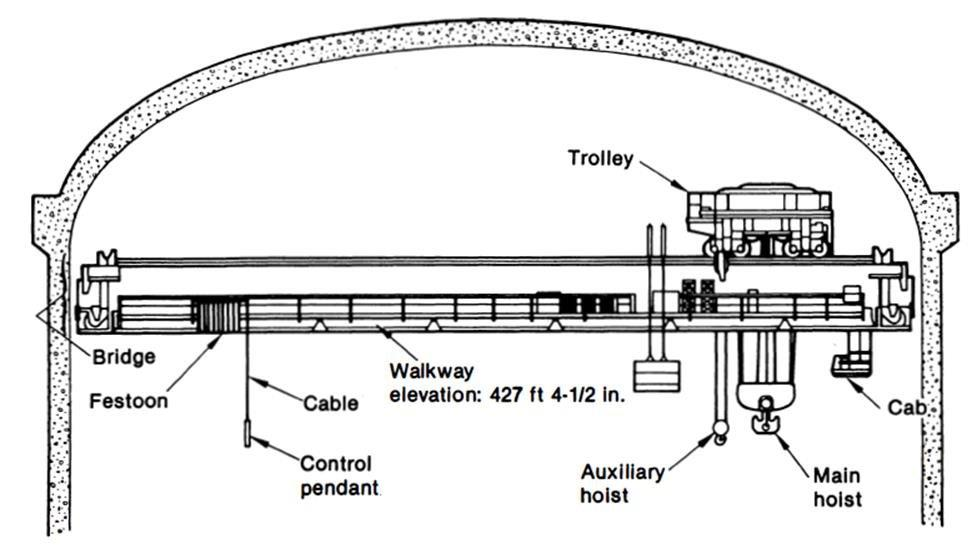
\includegraphics[height=8cm]{figures/rotary_crane.jpg}
    \caption{Rotary Overhead Crane~\cite{ONR-polar-crane}, or Polar Crane.  Three movements are possible in this system: polar crane rotation, trolley horizontal shift and charge lifting.}
    \label{fig:polar_crane}
\end{figure}

The attack demonstrator targets the polar crane's ICS. The operation of the polar crane is explained in this section. The rotary overhead crane (called thereafter polar crane) is a handling equipment which delivers and transports large components. It is for example used to lift and remove the reactor cover. The polar crane is only used during NPP shutdown, and its ICS is shutdown during the NPP operation. The polar crane equipment is standalone and is locally and manually operated by an operator. 

Two OT cyberattack scenarios were identified as possible ways of creating maximal damage and significant safety event:

\begin{itemize}
\item Shutdown of the polar crane with a charge above the reactor. This would create significant safety event with a possibility of the charge being drop above the reactor and breaking the first three barriers to radioactive release (i.e., fuel matrix, fuel cladding and boundary of the reactor coolant system)~\cite{international1996iaea}.
\item Activate charge lifting of the polar crane when it is in an overload situation caused by friction. For example this situation could be caused by friction when lifting a concrete slab which is placed above the confinement pool. If a cyberattacker detects it and  has full control over the PLC he could activate charge lifting to increase the overload which could either break the charge or make it fly.
\end{itemize}

\section{Industrial Control System and Programmable Logic Controller}

In this section are presented a cybersecurity introduction of the \emph{Industrial Control System} (ICS) and its major component — the \emph{Programmable Logic Controller} (PLC). 

\subsection{Industrial Control System (ICS)}

\emph{Industrial Control System} (ICS) is a network of interconnected systems that are designed to monitor and control industrial processes. Cybersecurity threats to ICS have far-reaching implications that can result in severe damage to property, loss of production, and even potential loss of life. Security of ICS thus requires a comprehensive approach that includes risk assessment, vulnerability identification, and implementation of appropriate protective measures.

ICS architecture are often modeled by the \emph{Purdue Model} represented in~\autoref{fig:purdue-model}. The attack surface is large and very diverse. It is large because the cyberattack could target any systems within the production network, the \emph{Industrial Control System} (ICS), the \emph{Supervisory Control And Data Acquisition} (SCADA), the corporate network etc. Attack surface is diverse because of the large number of different device types — actuators, sensors, \emph{Industrial Internet of Things} (IIoT) and smart devices, \emph{Remote Terminal Unit} (RTU), PLC, Engineering Workstation, \emph{Human-Machine Interface} (HMI), servers, switches, routers etc.


\subsection{Programmable Logic Controller (PLC)}

\emph{Programmable Logic Controller} (PLC), or similarly \emph{Programmable Automation Controller (PAC)}, is an industrial microprocessor-based controller made of a CPU, ROM, RAM, OS and a firmware. The PLC stacks are represented in~\autoref{fig:plc-stack}. The studied PLC is the \emph{Modicon M580} \emph{BMENOC0301} maintained by \emph{Schneider Electric}. It supports for example the following communication protocols: Modbus TCP, Ethernet IP, HTTP, FTP etc. The M580 is programmed by an engineering workstation by using the \emph{Unity Pro XL} software renamed as \emph{EcoStruxure Machine Expert} in the later versions. To program the PLC the closed-source Modbus/UMAS protocol is being used. 

\begin{figure}
    \centering
    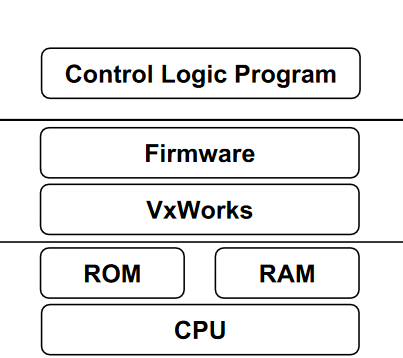
\includegraphics{figures/PLC-stacks}
    \caption{PLC Stacks of a PLC~\cite{Gao21} designed following the IEC 61131 standard. The Control Logic Program is the program executed by the CPU; it is a STM extension file for Schneider Electric programs. Considered firmware in this study is the Modicon M580 SV2.7 firmware. Considered CPU in this study is the Modicon M580. VxWorks is the real-time operating system running on the CPU.}
    \label{fig:plc-stack}
\end{figure}

\section{About Cybersecurity in ICS}

In the nuclear sector, most of the systems ensuring safety used to rely on analog devices. This technology adds a cybersecurity layer as analog devices are less complex and less connected. However, in the last decades, numerical devices with greater capabilities have penetrate the industrial market while the number of analog device manufacturers has dropped. This technology shift led to the success of several attacks~\cite{Drias15}. On another hand, the nuclear industry specifically focus on a defense-in-depth approach to ensure operational security.  

\subsection{Previous Major ICS Attacks in the Energy Sector}

\subsubsection{\emph{Stuxnet}}

\emph{Stuxnet} attack~\cite{stuxnetcode15},~\cite{Kushner13},~\cite{stuxnetdossier10} targeted the Iran's nuclear facilities and involved the use of a sophisticated worm exploiting multiple zero-day vulnerabilities and a rootkit technique to hide from antivirus. This OT cyberattack was designed to cause significant damage to the centrifuges responsible for enriching uranium by carefully tampering their speed to 1,064 cycles per second while keeping the attack stealth and persistent. The attackers used an attack cycle made of a combination of spear-phishing and network infiltration techniques to gain access to the targeted facility. Once inside, they deployed the \emph{Stuxnet} worm, which was capable of infecting both Windows operating systems and Siemens PLC while remaining undetected. 

\emph{Stuxnet} relied on several vulnerabilities to carry out its mission successfully. Primary vulnerability, the .LNK W32/\emph{Stuxnet} (CVE-2010-2568) vulnerability, took advantage of the use of USB drives to transfer data between systems. The associated exploit drops the trojan when the system automatically parses a shortcut file (.lnk)  which results in the execution of a malicious Control Panel module malware. This USB-based attack does not require to reprogram the USB peripheral. \emph{Stuxnet} approach allows replication by infecting USB thumb drives. \emph{NinjaCrane} is using another type of USB-based attack based on HID injection, which requires the presence of a programmable micro-controller in the USB peripheral. This adds a difficulty layer to the attacker and a less stealth attack but it allows in counter-part to infect any OS not implementing HID spoofing protection measures.

Another vulnerability that the attackers exploited was the weak authentication protocols of the \emph{Siemens} control systems. \emph{NinjaCrane} similarly exploits another vulnerability — \emph{ModiPwn} caused by a weak authentication of the \emph{Schneider Electric} communication protocol.

\subsubsection{\emph{Triton}}

The \emph{Triton} attack is a sophisticated cyberattack that targeted the safety instrumentation systems of a Saudi Arabian petrochemical plant in 2017. The \emph{Triton} attack started with the compromise of the plant’s network through phishing. The \emph{Triton} malware, once installed, was manipulating the safety controllers (the \emph{Triconex} PLC from \emph{Schneider Electric}) and the plant’s safety systems that monitor and detect incidents. By doing so, the attackers could have overridden the safety protocols, potentially resulting in an explosion or a toxic gas leak.

First vulnerability exploited was the human factor — the plant’s employees. The attackers used a spear-phishing email to trick an employee into downloading the \emph{Triton} malware, which then spread throughout the entire network. This highlights the importance of employees training in preventing cyberattacks.

One key vulnerability that the attackers exploited was the plant’s reliance on poorly-protected safety systems. The safety systems of the plant were not adequately secured against cyberattacks, and the use of legacy equipment, outdated firmware, and poorly configured network architecture made it easier for the attackers to breach the system and install the \emph{Triton} malware. The attackers were also successful in infiltrating the system because they had prior knowledge of the plant’s network topology, protocols, and industrial control systems, which helped them in crafting the malware to exploit the system’s vulnerabilities.

Similarities can be noted with the \emph{NinjaCrane} attack — the potentially catastrophic disaster of the cyberattack, human-factor role in the cyberattack, and prerequisite to reverse-engineer the PLC's communication protocol. This communication protocol is called \emph{TriStation} for the \emph{Triconex} PLC and Modbus/UMAS for the \emph{M580 PLC}. Also, the malware is, as for the \emph{NinjaCrane} attack, a python script compiled in an exe file using the \emph{py2exe} extension. Even if \emph{NinjaCrane} has persistence capabilities, it does not implement advanced hiding and anti-forensics techniques like \emph{Triton} does.

\subsection{From Operational Security to Cybersecurity in the Nuclear Industry}

The defense-in-depth approach taken by the nuclear industry during the control system design integrates operational security. The operational security can for example result into material and software redundancy, system qualification, human-supervision, mechanical stops, safety levels, priority on actuation control system etc. Those various mitigation barriers could also act as cybersecurity barriers. For example, a polar crane can integrate a kinematics line monitoring system responding to motor overspeed or engine backfire. As another example, a polar crane can integrate a wired emergency stop with highest priority order to shutdown the polar crane. Those defense-in-depth barriers won't protect directly against the \emph{NinjaCrane} attack but will prevent the attack to set a high polar crane's rotation speed or to deviate visually from normal operation as the automation operator will activate an emergency stop as soon as the the polar crane behaves differently than expected. 


\subsection{Security of the \emph{Modicon M580}}

\emph{Schneider Electric} lists all released vulnerabilities and their state \cite{schneider-portal-vuln}. As a first observation, the number of discovered vulnerabilities on the \emph{M580} is around ten per year. Moreover, the average time to patch a vulnerability is between two and four years. Unfortunately, patch deployment implies some code modification and thus requires a system re-qualification. It also requires industrial process stop. For those reasons a patch deployment can take more than a decade to be applied.

Among those vulnerabilities, the approach was to choose a communication protocol vulnerability as it allows to perform lateral movement from engineering workstation to PLC. Compromising directly the PLC would have require an access to the PLC. But the access to an ICS is physically restricted and PLC are usually placed into physically locked electrical cabinet. Moreover, in case of communication protocol vulnerability, remediation requires PLC firmware update and Unity Pro engineering workstation update. As date of 12 March 2023, Schneider Electric reports that a replay attack on the \emph{Modicon M580} is still possible \cite{schneider-replay-attack} and advises to harden the engineering workstation.

\subsection{Overview on USB-related Threats}

Number of USB-based attacks tends to increase over time and be more diverse~\cite{Nissim17}. \emph{NinjaCrane} makes use of a USB-based attack that can be classified as programmable micro-controller hardware-based attack. Many such attack-capable devices are available on the market, e.g., \emph{BadUSB}, \emph{BadUSB 2}, \emph{Rubber Ducky}, \emph{USBHarpoon}, \emph{OMG Cables}, \emph{USB Ninja}, \emph{Bash Bunny} etc.

\emph{NinjaCrane} infects the ICS with the use of a \emph{USB Ninja} cable type-C (or a maliciously modified mouse) that would be plugged to the engineering workstation. The USB Ninja cable and the malicious mouse are \emph{Human Interface Devices} (HID) spoofing device injecting keyboard key-frames. For the USB Ninja cable, the attack can be triggered over Bluetooth and in its professional version the key-frames can even been sent over Bluetooth. Moreover, the \emph{USB Ninja} cable is a working charging cable indistinguishable, at first glance, from a conventional charging cable. For the maliciously tampered mouse, any HID-capable device with extensive memory or embedded wireless connection can be placed in the mouse to execute the malware. Except from its weights, the mouse is indistinguishable from a conventional mouse.

\emph{Human Interface Device} (HID) spoofing device~\cite{epstem1225679} mimics legitimate HID to trick the computer to believe a keyboard is attached, the device then sends pre-configured keystrokes. To mimic a legitimate HID, the spoofing device operates an USB transport layer enumeration. It will then initiate data exchange under the format of input/output reports where the input report can contain keystrokes or mouse click to inject. As those keystrokes injection are impractical to deploy an advanced threat, the injected keystrokes generally perform an USB Drive-By attack in order to execute a downloaded malware.
%%%%%%%%%%%%%%%%
\chapter{Threat Model}
%%%%%%%%%%%%%%%%
\label{chapter:threat-model}

This chapter introduces the considered threat model for the \emph{NinjaCrane} attack. This includes a description of the adversary model and its attack surface. 

\section{Adversary Model}

The system under attack is the polar crane's ICS. The choice made by the adversary is justified as follow. Control and regulation functions in normal operation are generally made redundant with independent and diversified systems, and some components are non-electrical analog devices making it hard to compromise. However, during NPP shutdown less securely-proofed systems are used like the polar crane and can be seen as a weaker link. 

The adversary type considered is an external adversary with medium capabilities such as hacktivists, hacking collectives or non-state cyber-terrorists. As such, adversary is considered to have no physical access to the NPP station, and would require unintentional insider threat to enter in the air-gap polar crane's ICS. Moreover, considered attacker is not highly skilled and would not exploit any 0-day vulnerability. However, the considered adversary has medium resources and has the capacity to chain known vulnerabilities and has an access to a M580 PLC, publicly accessible in the market, to reverse engineer it and test the cyberattack. As an hypothesis, some leaked information regarding the polar crane's ICS is assumed e.g., the supply chain leaked material references, unintentional data leak on social media from employee helped to identify automation operators interacting with the polar crane etc.

The campaign objective is industrial sabotage by system tampering up to destruction. More precisely, the adversary's goal is to slow down or to keep the energy production of the NPP stopped in order to inflict economical loss or corporate shaming. As a recall, a reactor unit with a 900 MW capability generates around 3 M dollars per day. The cyberattack is performed during the periodic nuclear unit shutdowns and when the polar crane equipment is being used. Tampering or stopping the normal operations of the polar crane will delay the resumption of the energy production.

The campaign vehicle is an USB physical media such as a maliciously tampered USB cable or a maliciously tampered mouse. The infected USB physical media is brought to the NPP station via spear-phishing or supply chain compromise e.g., sending an USB Ninja cable or a malicious mouse to the automation operator as a fake gift from a subcontractor or a colleague.

The campaign weapons are HID spoofing and Modbus/UMAS exploit. The payload delivery is a keystrokes injection and a pre-compiled executable file. 

The payload capabilities are keystrokes injection on the engineering workstation, data exfiltration of the information products, lateral movement from engineering workstation to PLC, Command and control by triggering on time the attack on the PLC and finally Denial-of-Service (DoS) of the PLC and polar crane to stop the use of both. 

\section{Attack Surface}

This section describes the attack surface of the polar cane's ICS architecture. \autoref{fig:data_flow_diagram} represents a Data Flow Diagram of an ICS by listing the common assets, security controls and threat actors. 

All components of the ICS have a physical access control, i.e., safety gantry, key system etc. Three scenarios for the external intrusion could be consider:

\begin{itemize}
    \item Intrusion via the \emph{Information System} (IS), e.g., an employee plugs his own infected laptop to the corporate network.
    \item Intrusion via the \emph{Supervision Network} (SCADA), e.g., an operator on site plugs a found USB-capable device on the log servers or on an engineering workstation.
    \item Intrusion via the \emph{Production Network}, e.g., an adversary maliciously tampers an electronic actuator before it is delivered on site. 
\end{itemize}

By assuming that the supply chain of the polar crane is trusted, only the first two intrusions remain as the ICS is thus considered as clean after setup. The second scenario is the one kept in the following chapters for practicality, i.e., network architecture connecting the ICS and the IS is complex and is generally considered as an unidirectional network from ICS to IS.
%%%%%%%%%%%%%%%%
\chapter{Testbed Overview}
% TODO
%%%%%%%%%%%%%%%%

This chapter describes the testbed of the \emph{NinjaCrane} attack. This testbed is used in the Evaluation \Cref{chapter:evaluation} to test the attack.  

\section{The Polar Crane as a Physical Process}

For illustration purpose the attack is performed on a sketch in LEGO\texttrademark\ of the polar crane. This sketch has been made by B. Allard and T. Cassas with the first goal being to introduce a practical control system and to create a training on software and equipment qualification. 

\subsection{Description}

The sketch of the polar crane can be found in~\autoref{fig:polar-crane}. This sketch made in LEGO\texttrademark\ is not to scale. The polar crane is composed of three BLE Hubs controlling the crane's rotation, trolley's shift, and charge lift-up. The cyberattack will target the crane's rotation in order to stop it.   

\subsection{Components}

Here is the list of the sketch components (sensors and actuators):

\begin{itemize}
    \item 3 $\times$ LEGO\texttrademark\ Powered Up Technic Hub (88012)
    \item 3 $\times$ LEGO\texttrademark\ Powered Up (88007) Color \& Distance Sensor (e.g., computes the angular position of the polar crane to initialize it)
    \item 1 $\times$ LEGO\texttrademark\ Powered Up Technic XL Motor (88014), used for charge lift-up.
    \item 1 $\times$ LEGO\texttrademark\ Powered Up Technic Large Motor (88013), used for trolley shift.
    \item 4 $\times$ LEGO\texttrademark\ Powered Up (88011) Train Motor, used for polar crane rotation.
\end{itemize}

\section{Electrical Cabinet}

This section presents the physical Electrical Cabinet used in the testbed. The cabinet contains the PLC and the HMI and can be considered as representative as it has been qualified following the \href{https://www.afcen.com/en/rcc-e/187-rcc-e.html}{AFCEN RCC-E} nuclear standard (i.e., the electrical cabinet used in this testbed could be placed in a NPP site). 

\subsection{Description}

The PLC M580 is connected to the ESP32 via the MAX232 converter (RS232 to TTL serial respectively). The ESP32 is communicating over \emph{Bluetooth Low Energy} (BLE) to the Bluetooth Hubs of the polar crane. This part is not representative of reality but the success of \emph{NinjaCrane} cyberattack is independent from this choice.

\subsection{Main Components}

\begin{itemize}
    \item 1 $\times$ HMI: Magelis HMIIG3U
    \item 1 $\times$ CPU: Modicon M580 (BMEXBP582040), firmware v2.70 (07/2018)
    \item 1 $\times$ Rack: Modicon X80, 12 slots, Ethernet backplane (BMEXBP1200)
    \item 1 $\times$ Fiber converter module: Modicon X80, single mode (BMXNRP0201)
    \item Diverses I/O modules used for buttons and lights — not itemized here
    \item 1 $\times$ ESP 32-WROOM-32
    \item 1 $\times$ Maxim Integrated Products MAX232 IC
\end{itemize}


\section{Engineering Workstation}

\subsection{Description}

The engineering workstation is connected to the PLC via an Ethernet connection. The protocol used to program and communicate is Modbus/UMAS over TCP/IP. This connection can be considered as representative of reality. However, the engineering workstation is assumed to be connected to the internet at some point for malware download (if the USB Ninja cable is being used) and data leakage during the cyberattack. This could for example happen if the automation operator connects the workstation to download a driver or update a system. Unity Pro is the software that modifies, compiles and uploads the program on the PLC. The program is stored in a .STU file.

\subsection{Characteristics}

The engineering workstation is a desktop computer with the following characteristics:

\begin{itemize}
    \item Operating System: Windows 10 Professional 22H2 (build 19045.2604)
    \item Antivirus: Avast Antivirus Free (Version 23.3.8047.782)
    \item WiFi Adapter: WiFi Adapter RoHS NBS WFLD01
    \item Software:
    \begin{itemize}
        \item Unity Pro XL V13.1 - 180823C (Schneider Electric Industries SA). Documentation of Unity Pro v13.1 software \cite{docUnityPro}.
    \end{itemize}
    \item Admin user account
\end{itemize}

\section{Adversary's Tools}

\subsection{Laptop}

\begin{itemize}
    \item Operating System: Windows 11 Professional 22H2 (build 22621.1702)
    \item Software:
    \begin{itemize}
        \item Python 3.11.1
        \item nRF Connect 4.1.2
        \item Wireshark 4.0.6
    \end{itemize}
    \item Admin user account
    \item Bluetooth Sniffer Dongle : Nordic Semiconductor nRF 52840
\end{itemize}

\subsection{USB Ninja Cable}

USB Ninja cable from Lab401 can be configured with the  \href{https://github.com/4d4c/USBNinja}{\emph{USBNinja github}}. The USB Ninja cable is a regular USB cable that can be triggered via a wireless remote controller to execute a pre-compiled payload. The payload is uploaded via the Arduino IDE. 

\subsection{Malicious Mouse}

The malicious mouse is made of a regular mouse in which were added a USB hub to multiplex the serial connection to add a microcontroller. The microcontroller then act as a HID-capable device and execute a pre-compiled payload.

The electric schematic can be found in~\autoref{fig:infected-mouse-wiring}. The design of the maliciously modified mouse offers flexibility as any microcontroller with micro USB type B connector can be inserted in the mouse. The \emph{Adafruit Trinket M0} is the microcontroller used in this MSc thesis.  

\section{Network Architecture}

The overall network architecture of the testbed is described in details in~\autoref{fig:setup}. The engineering workstation, connected in Ethernet to the PLC, uploads the program. The engineering workstation programs the HMI with the \emph{Vijeo} software by temporarily connecting in serial to the HMI. The HMI and the PLC are connected in Ethernet allowing the PLC to send the variables state to the HMI and the HMI to send command orders to the PLC. The PLC program relays those orders to the ESP32 that interprets them and activates the corresponding BLE Hubs to control the polar crane. 


%%%%%%%%%%%%%%%%
\chapter{Design}
% Introduce and discuss the design decisions that you made during this project. Highlight why individual decisions are important and/or necessary. Discuss how the design fits together.
% This section is usually 5-10 pages.
%%%%%%%%%%%%%%%%

This chapter discusses the design choices made for the \emph{NinjaCrane} attack like the attack cycle, and some weaknesses of the Modbus/UMAS communication protocol.

\section{Attack Cycle}

In the following subsections are described the different steps taken by the attacker. The attack tree is described in~\autoref{fig:atk-tree}. The entry point considered is a physical device connected to the air-gap network. For example, the compromise of the supply chain can induce a device to be brought into the the NPP site and be connected to the engineering workstation. This device will infect the engineering workstation via an HID attack and run a malware. The malware performs lateral movement to the PLC via a MITM attack to change the PLC's internal variables. 

\section{Entry Points}

As the control panel cabinet is locked and devices in rotary overhead crane are considered as secure (see~\Cref{chapter:threat-model}), the adversary could target only two systems i.e. the engineering workstation or the BLE communication. Taking back the initial network architecture, adversary's entry points are represented in~\autoref{fig:sketch-entry-pt}. For a better representativeness — there's no LEGO\texttrademark\ BLE in a NPP station — the choice has been made to target the engineering workstation as an entry point. Moreover, in the testbed, an attacker could easily connect with the BLE hub with a phone as there is no protection in the LEGO\texttrademark\ Wireless Protocol.

\begin{figure}[H]
    \centering
    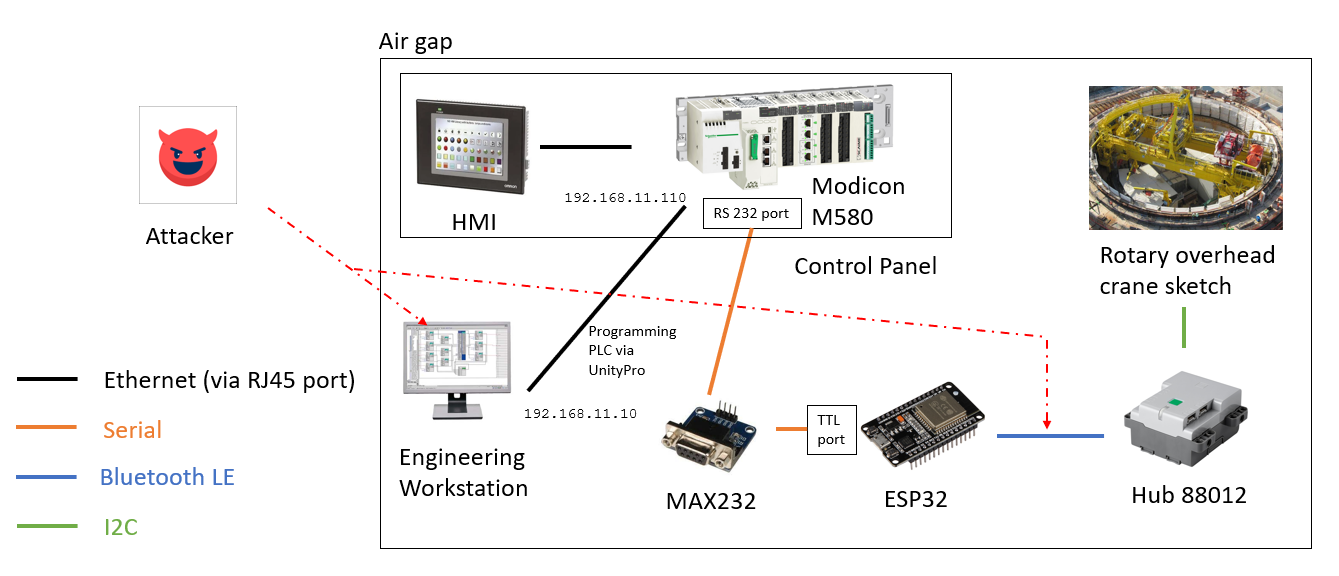
\includegraphics[width=\linewidth]{figures/Sketch.PNG}
    \caption{Adversary's Possible Entry Point}
    \label{fig:sketch-entry-pt}
\end{figure}

\subsection{Malicious USB Device Delivery}

The first step of the attack is to bring a compromised USB device to be connected to the engineering workstation. A spear-phishing attack can take the form of the effective USB drop attack — "Users Really Do Plug in USB Drives They Find"~\cite{Tischer16}. The supply chain compromise could exploit vulnerabilities in the Integrated Circuit (IC) Systems development life cycle (SDLC) that can lead to a compromised USB end-product~\cite{Tun22}~\cite{Melnyk22}. More details on the how a physical media would be brought and why it would be plugged in won't be discussed any further. The next Chapter will discuss two different malicious USB devices that can be used as a possible entry point to infect the workstation. 

\subsection{Engineering Workstation Infection}

Engineering workstation are used by automation operators — who may not be trained enough regarding the security policy — to program the PLC. The engineering workstation could be infected by either a malicious mouse or a USB Ninja cable. Both could contain a pre-compiled payload that will be described in further details in the next Chapter. The goal of the infection is to take the control over the communication with the M580 in a persistent and stealth way. To this extent, a MITM attack could be setup to modify the PLC's variables state and thus take the control of the polar crane.

\section{Communication Between the M580 and the Engineering Workstation}

In this section is described the communication protocol between the PLC and the workstation i.e., the UMAS protocol.

\subsection{Unity Pro and UMAS Protocol}

The communication between the M580 PLC and the engineering workstation follows the UMAS/Modbus protocol over TCP/IP. The UMAS protocol is specific to Unity Pro — the software used to program the \emph{Modicon} PLC — and is a proprietary communication protocol from \emph{Schnieder Electric}. The overall packet format is ordered as follow:

\begin{enumerate}
    \item \textbf{Ethernet}: \texttt{Destination MAC address, Source MAC address, Type}
    \item \textbf{IP}: \texttt{Version}, ..., \texttt{Length Id}, \texttt{Checksum}, \texttt{Source IP address}, \texttt{Destination IP address}
    \item \textbf{TCP}: \texttt{Source port}, \texttt{Destination port}, \texttt{Sequence number}, \texttt{Acknowledgment number}, \texttt{Flags}, \texttt{Window}, \texttt{Checksum}
    \item \textbf{Modbus TCP}: \texttt{Transaction Id}, \texttt{Protocol Id}, \texttt{Length}, \texttt{Unit Id}
    \item \textbf{Modbus}: \texttt{Function code} (e.g., \texttt{0x5A} for \emph{Unity Pro}), \texttt{UMAS data}
\end{enumerate}

Thanks to the work from CICLAB Laboratory of the University of Leon~\cite{umas}, the UMAS protocol has been almost completely reversed. According to this, UMAS packet takes the following request/response format:
\begin{itemize}
    \item Modbus packet format from workstation to PLC (i.e., request): \texttt{0x5A}, \texttt{session}, \texttt{UMAS function code}, \texttt{data}
    \item Modbus packet format from PLC to workstation (e.g., response): \texttt{0x5A}, \texttt{session}, \texttt{status code} (i.e., \texttt{0xFE}), \texttt{data}
\end{itemize}

Below are some remarks regarding the UMAS protocol.

\begin{itemize}
    \item The \texttt{session} token is used to authenticate the workstation's packets and is fixed until the end of the communication. This token is set to \texttt{0x00} when the authentication is disabled or for the first non-authenticated packets used to create this token. In the next part, it is assumed that authentication is enabled. To compute the \texttt{session} token the workstation must use the UMAS reservation mechanism. After this, workstation is synchronized to modify the PLC’s program and variables.
    \item The \texttt{UMAS function code} is used by the workstation to specify the request function (e.g., \texttt{READ\_MEMORY\_BLOCK}, \texttt{READ\_VARIABLES}, \texttt{KEEP\_ALIVE}, ...~\cite{umas}).
    \item The \texttt{status code} is used by the PLC to notify any error (i.e., \texttt{0xFD}) or a success (i.e., \texttt{0xFE})
\end{itemize}

An example of UMAS packet over TCP/IP can be found in~\autoref{fig:modbus-packet}.

\begin{figure}[H]
    \centering
    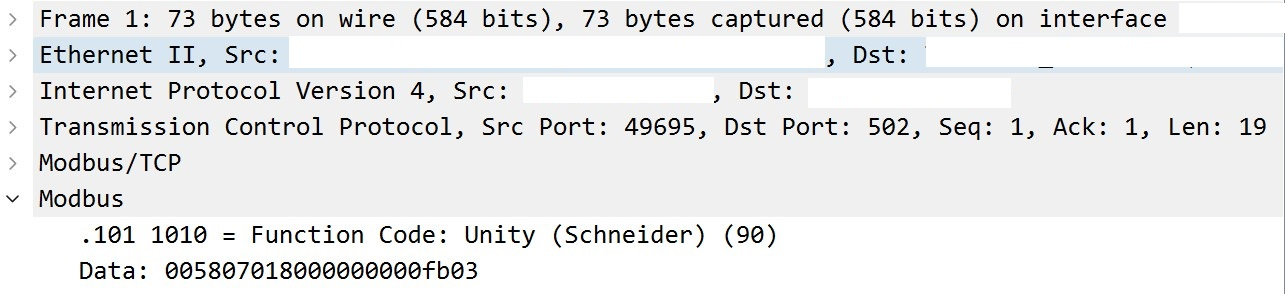
\includegraphics[width=0.8\linewidth]{figures/typical_modbus_packet.jpg}
    \caption{A Modbus/UMAS packet over TCP/IP. Regarding the Modbus packet; function code is $90_{10} = \texttt{0x5A}$, the packet is not authenticated (session is \texttt{0x00}), it is a request sent by the workstation to check the PLC status (request \texttt{0x58})}
    \label{fig:modbus-packet}
\end{figure}

\subsection{The Unity Pro Protection Passwords}

Four different passwords can be set by the engineering workstation within Unity Pro:
\begin{itemize}
    \item \textbf{Application Protection}: Password protecting the CPU and Unity Pro by preventing modification, upload and program opening. UTF-16-le encoding of this password will be denoted as $\texttt{app\_pwd}_{\textrm{(utf-16-le)}}$ hereafter.
    \item \textbf{Program Unit, Section and Subroutine Protection}: Password protecting the program sections and program units (from writing and reading). UTF-16-le encoding of this password will be denoted as $\texttt{prgrm\_pwd}_{\textrm{(utf-16-le)}}$ hereafter.
    \item \textbf{Data Storage Protection}: Password preventing malicious access to the data storage of the SD memory card. UTF-16-le encoding of this password will be denoted as $\texttt{data\_pwd}_{\textrm{(utf-16-le)}}$ hereafter. Default password is "datadownload".
    \item \textbf{Firmware Protection}: Password preventing malicious access to the module firmware via FTP. UTF-16-le encoding of this password will be denoted as $\texttt{firmware\_pwd}_{\textrm{(utf-16-le)}}$ hereafter. Default password is "fwdownload".
\end{itemize}

\subsection{Communication Phases in Normal Operation}

This subsection details the communication phases between the workstation and the PLC in normal operation. A first stage is to setup the passwords (see Password Setup Phase), send the project information (see Project Setup Phase), and then upload the program (see Program Upload Phase). In a second stage, the engineering workstation will connect (again) to the PLC (see Connection Phase), get back from the PLC the project information running on it (see Information Gathering Phase), make a reservation (see Making a Reservation Phase), and finally send command to the PLC e.g., start PLC, modify variables, or upload a new program (see Send Command Phase). 

\subsubsection{Password Setup}
\label{subsubsection:pwd-setup}

When setting up new passwords, the workstation, via the \texttt{UPLOAD\_BLOCK} function (\texttt{0x31}), sends to the PLC the base64 encoding of three bytes sequence; \texttt{salt2}, \texttt{hash1}, and \texttt{hash2} defined in~\autoref{equ:define-hash}. This phase assumes that the engineering workstation already established a connection with the PLC.

\begin{align}
\label{equ:define-hash}
\begin{split}
    \texttt{hash1} &:= \textrm{SHA256}(\texttt{salt1} + \texttt{data\_pwd}_{\textrm{(utf-16-le)}}) \\
    \texttt{hash2} &:= \textrm{SHA256}(\texttt{salt2} + \texttt{firmware\_pwd}_{\textrm{(utf-16-le)}})
\end{split}
\end{align}

Where \texttt{salt1} and \texttt{salt2} are random 48-bits length bytes sequence generated by Unity Pro and sent in base64 to the PLC.

An example of a UMAS packet over TCP/IP sent when new passwords are set can be found in~\autoref{fig:modbus-packet-setup-pwd}.

\begin{figure}[H]
    \centering
    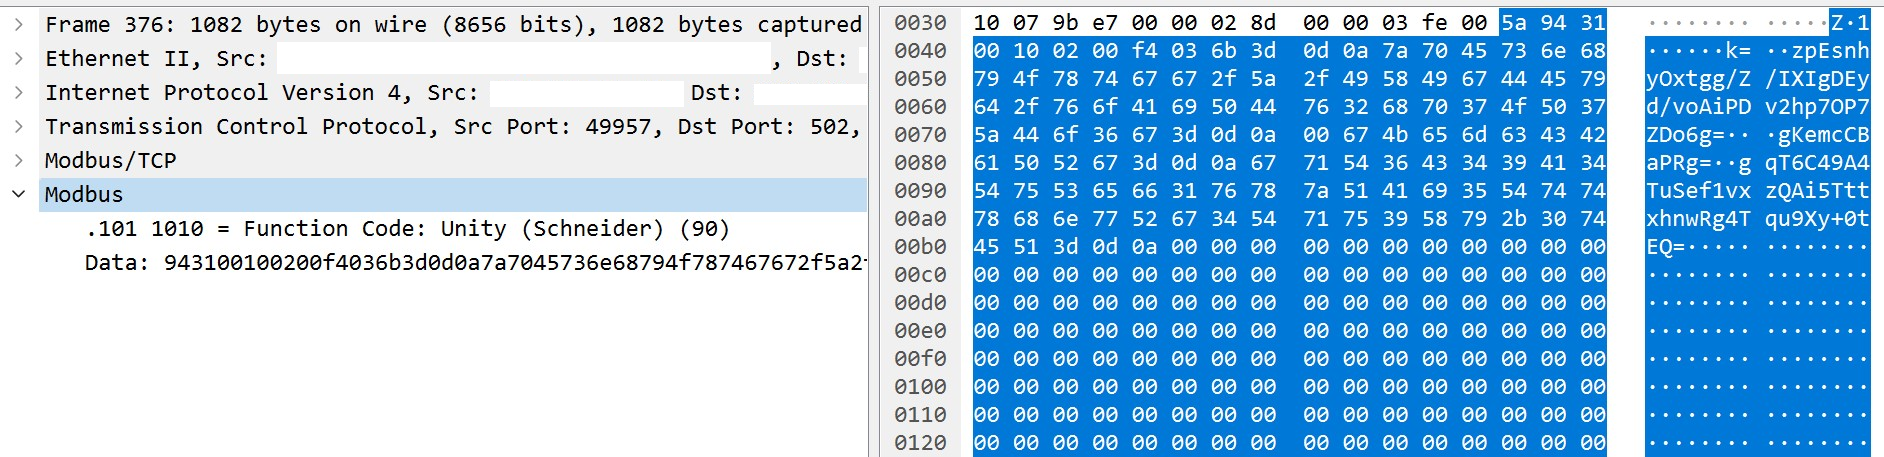
\includegraphics[width=\linewidth]{figures/setup-pwd}
    \caption{A Modbus/UMAS packet sent over TCP/IP to modify the passwords with the following values; $\texttt{hash1} := \textrm{SHA256}(\texttt{salt1} + \texttt{datadownload}_{\textrm{(utf-16-le)}} = \texttt{zpEsnhyOxtgg/Z/IXIgDEyd/voAiPDv2hp7OP7ZDo6g=}_{\textrm{(base64)}}$. $\texttt{salt2} := \texttt{gKemcCBaPRg=}_{\textrm{(base64)}}$ and $\texttt{hash2} := \textrm{SHA256}(\texttt{salt2} + \texttt{fwdownload}_{\textrm{(utf-16-le)}}) = \texttt{gqT6C49A4TuSef1vxzQAi5TttxhnwRg4Tqu9Xy+0tEQ=}_{\textrm{(base64)}}$ }
    \label{fig:modbus-packet-setup-pwd}
\end{figure}


\subsubsection{Setup Phase}

\label{subsec:setup-phase}

When uploading a new program onto the PLC, the workstation uses the \texttt{UPLOAD\_BLOCK} function to write information regarding the project. Below is the list of the sent information according to an example of packet sent when uploading project information (see~\autoref{fig:modbus-packet-setup-phase}.).

\begin{itemize}
    \item Project name: \texttt{Projet}

    \item "Encrypted" program password: $\textrm{enc}(\texttt{prgrm\_pwd}) = \texttt{37713D7S}$. The "encryption" is detailed in the next paragraph.
    
    \item $\texttt{salt3} := \texttt{6Umv13jYhak=}_{\textrm{(base64)}}$
    
    \item $\begin{aligned}[t]
        \texttt{hash3} :&= \textrm{SHA256}(\texttt{salt3}+\texttt{app\_pwd}_{\textrm{(utf-16-le)}}) \\ &= \texttt{XBhpWAvOQj/l67B7SV00wh03M+7KO/sMstr2Teed/54=}
    \end{aligned}$
    
    \item Unity Pro software version: \texttt{V13.1}
    
    \item Computer name: \texttt{DESKTOP-8NOLHQU}
    
    \item Program file path. This the path to the .STU file that is being uploaded on the PLC: \texttt{E:$\backslash$PROJET\_2$\backslash$P...OM\_BA.STU}
    
    \item $\texttt{salt1} := \texttt{50iiBJuyhpk=}_{\textrm{(base64)}}$. This salt is fixed (i.e., it stays fix over different password changes).
    % TODO
    \item $\begin{aligned}[t]\texttt{hash1} :&= \textrm{SHA256}(\texttt{salt1} + \texttt{datadownload}_{\textrm{(utf-16-le)}} \\ &= \texttt{zpEsnhyOxtgg/Z/IXIgDEyd/voAiPDv2hp7OP7ZDo6g=}_{\textrm{(base64)}}\end{aligned}$
    \item $\texttt{salt2} := \texttt{gKemcCBaPRg=}_{\textrm{(base64)}}$
    \item $\begin{aligned}[t]\texttt{hash2} :&= \textrm{SHA256}(\texttt{salt2} + \texttt{fwdownload}_{\textrm{(utf-16-le)}}) \\ &= \texttt{gqT6C49A4TuSef1vxzQAi5TttxhnwRg4Tqu9Xy+0tEQ=}_{\textrm{(base64)}}\end{aligned}$
\end{itemize}

\begin{figure}[H]
    \centering
    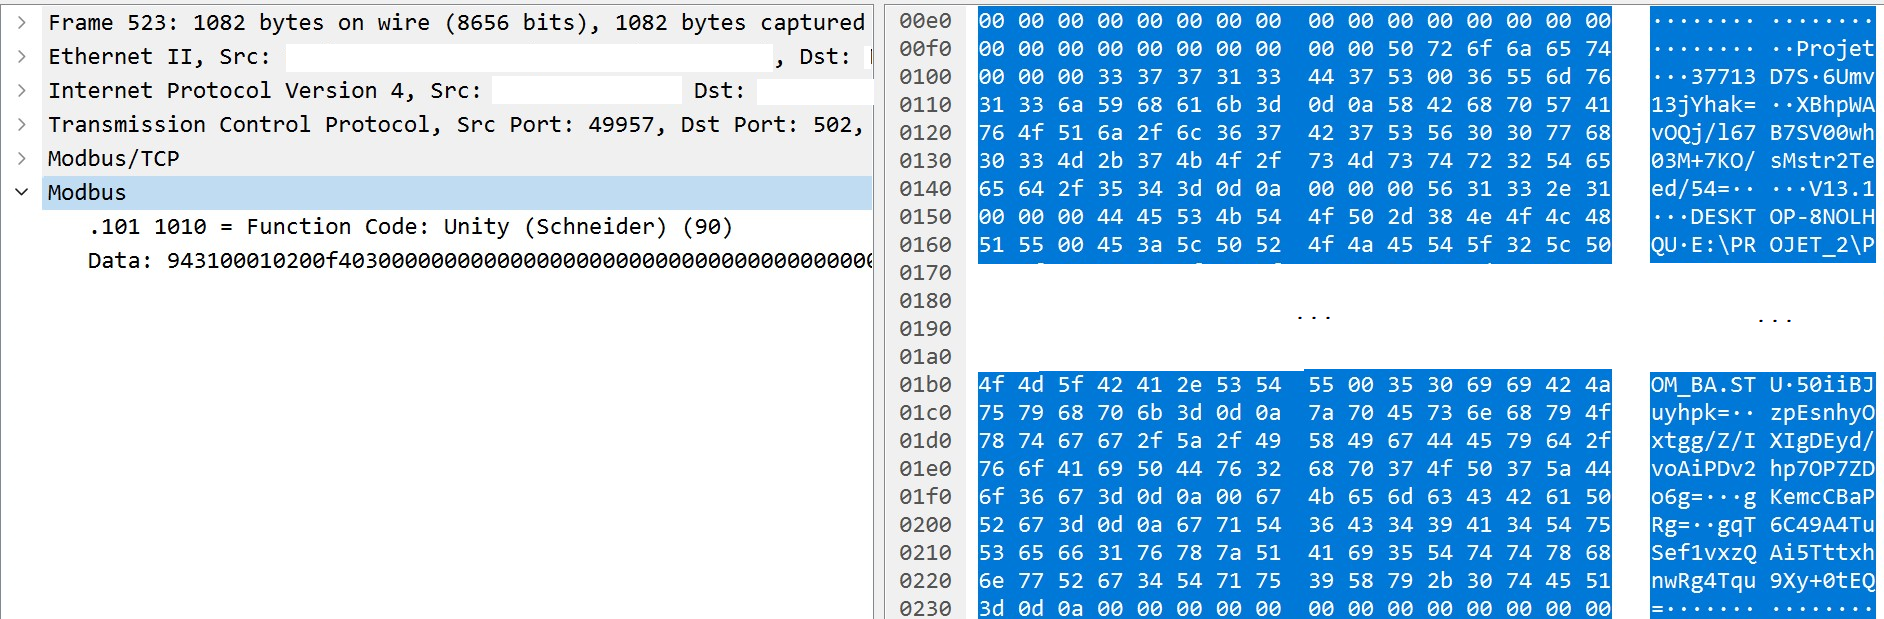
\includegraphics[width=\linewidth]{figures/project-info}
    \caption{A Modbus/UMAS packet sent over TCP/IP to modify project information.}
    \label{fig:modbus-packet-setup-phase}
\end{figure}


The "encryption" (as called by Schneider Electric) algorithm used to send Program Unit, Section and Subroutine Protection password is a custom-made hash algorithm. It has been reversed by Nicholas Miles~\cite{modipwn} and a simplified version of it is described in~\Cref{algo:pwd-hash}. This simplified version assumes that the password is only made of Basic Latin character (e.g., first Unicode Block).

For $x \in \mathbb{N}$, let $f$ be defined as:

\begin{multline}
    \label{equ:define-f}
    f:x\mapsto (x \bmod{2})((x \bmod{16} + 72)) + \\ (x + 1 \bmod{2})((x\bmod{16}\bmod{11}\bmod{2})(x\bmod{16}+48) + \\ (x\bmod{16}\bmod{11} + 1 \bmod{2})(x\bmod{16} + 55))
\end{multline}

\begin{algorithm}[H]
\caption{Password hash}
\label{algo:pwd-hash}
\hspace*{0pt} \textbf{Assumption:} The plaintext password is encoded in utf-8 and is only made of Basic Latin characters \\
\hspace*{0pt} \textbf{Input:} $p = p_0,....,p_{\textrm{len}(p)-1}$ (plaintext password), where $p_i$ is a utf-8 character (i.e, a hex number) for $i \in \{0, ..., \textrm{len}(p)-1\}$\\ 
\hspace*{0pt} \textbf{Output:} $e = e_0,....,e_{\textrm{len}(p)-1}$ (password hash of same length as password) \\ 
$e_{-1} \gets 0$ \\
$S \gets \sum_{i=0}^{\textrm{len}(p)-1}p_i$ \\
\For{$i\gets$ $0$ $\KwTo$ $\textrm{len}(p)-1$}{
    $e_i \gets f(e_{i-1}*i + S + p_i*(i+1))$ where $f$ was defined previously in~\autoref{equ:define-f}
}
$e \gets e_0, ..., e_{\textrm{len}(p)-1}$ \\
\Return $e$
\end{algorithm}

The work of M. Miles has been extended to break the hash algorithm. To find back a pre-image of $e$ we need to solve the following equations system for $S, p_1, p_2, ..., p_{\textrm{len}(p)-1}$,

\begin{equation}
    \begin{cases}
      e_0 = f(S)\\
      e_1 = f(p_0 + p_1 + S)\\
      e_2 = f(2*(p_1 + p_2) + S)\\
      ... \\
      e_i = f(i*(p_{i-1} + p_i) + S)\\
      ... \\
      e_{\textrm{len}(p)-1}= f((\textrm{len}(p)-1)*(p_{\textrm{len}(p)-1-1}+ p_{\textrm{len}(p)}) + S)\\
    \end{cases}\,.
\end{equation}

And then using the definition of $S$ we obtain $p_0 = S - \sum_{i=1}^{\textrm{len}(p)-1}p_i$. The code can be found in the \emph{NinjaCrane github}~\cite{MyGithub}. 


Moreover, by using SHA256  as such: $\textrm{SHA256}(\textrm{salt} + \textrm{password})$ and sending it in clear; the following vulnerability observations can be made regarding an active attacker: 

\begin{enumerate}
    \item The communication is flawed by design as the salt is also sent in clear. More precisely, the attacker can leave the sent salt unmodified but tampers the sent $\textrm{SHA256}(\textrm{salt}+\textrm{password})$ into $\textrm{SHA256}(\textrm{salt}+\textrm{tampered\_password})$, where $\textrm{tampered\_password}$ is a password chosen by the attacker. 
    \item  Making use of a hash of concatenation rather than a HMAC could lead to an extension attack. For example an adversary tampering the sent $\textrm{SHA256}(\textrm{salt}+\textrm{password})$ into $\textrm{SHA256}(\textrm{salt}+\textrm{password}+\textrm{adding\_characters})$ will modify the correct password into  $\textrm{password}+\textrm{adding\_characters}$.
    \item  By modifying the salt the adversary could perform a collision attack. For example let's assume that the salt is equal to $\textrm{salt1} + x$ then
    we have that $\textrm{SHA256}(\textrm{salt}+\textrm{password})=\textrm{SHA256}(\textrm{salt1}+x+\textrm{password})$. A collision hash is created by removing $x$ at the end of $\textrm{salt}$ and by adding $x$ to the beginning of $\textrm{password}$.
\end{enumerate}

\subsubsection{Program Upload Phase}

Once the password setup and the information regarding the project have been sent to the PLC, the engineering workstation will upload the program using the \texttt{UPLOAD\_BLOCK} request function. 

\subsubsection{Connection Phase}

The reservation phase establishes the connection between the PLC and the engineering workstation. To do so, the engineering workstation sends a random nonce (denoted  \texttt{client\_nonce}) and the PLC replies by sending another random nonce (denoted  \texttt{server\_nonce}) as shown in~\autoref{fig:nonces}.

\begin{figure}[H]
    \centering
    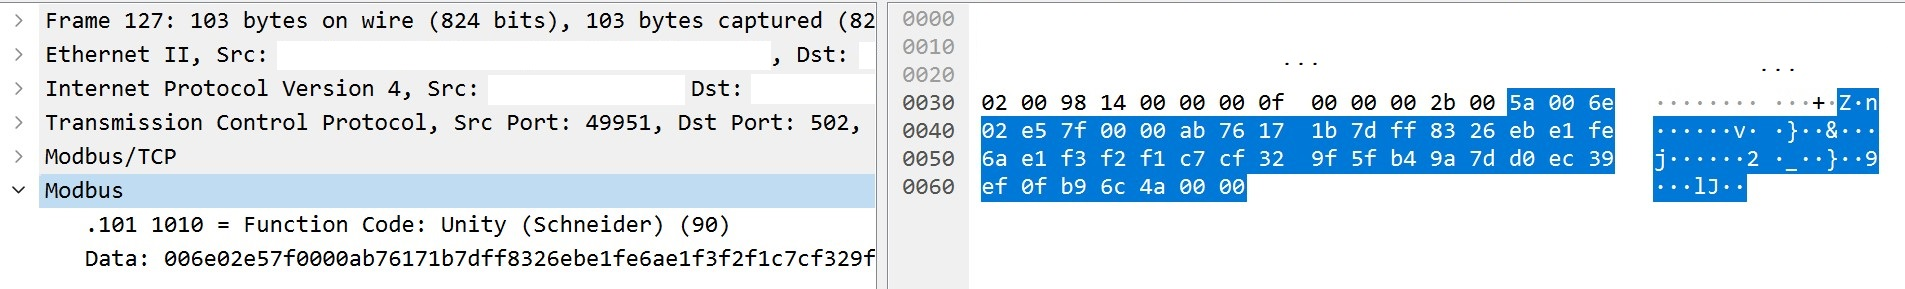
\includegraphics[width=\linewidth]{figures/client_nonce.jpg} 
    \\ \vspace{0.5cm}
    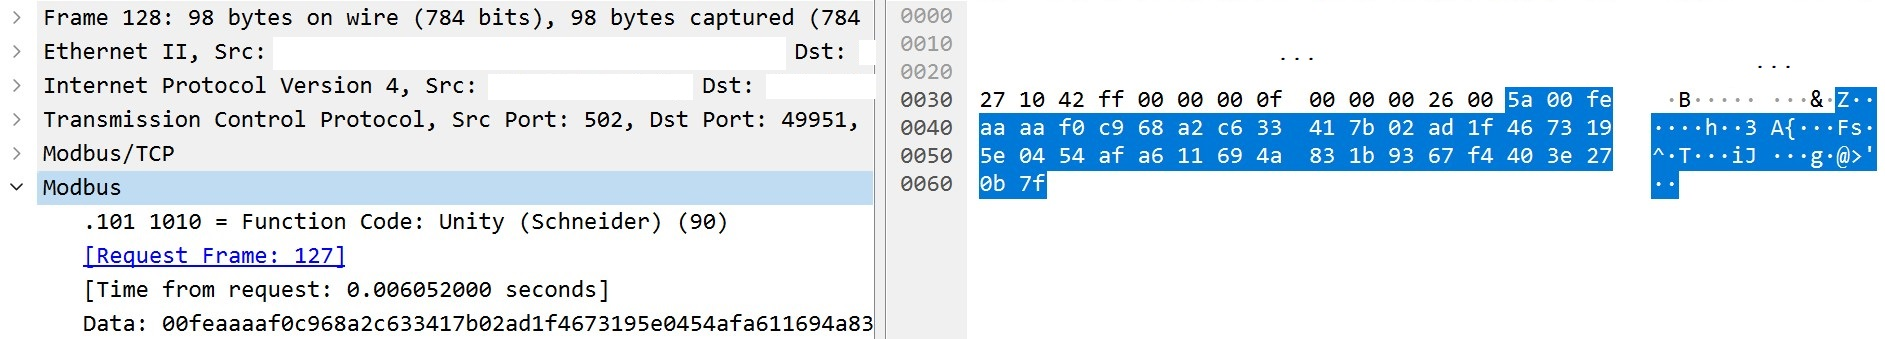
\includegraphics[width=\linewidth]{figures/server-nonce.jpg}
    \caption{Top: Client (i.e., workstation) Nonce is \texttt{0xab76...6c4a}. Bottom: Server (i.e., PLC) Nonce response is \texttt{0xf0c9...0b7f}.}
    \label{fig:nonces}
\end{figure}

\subsubsection{Information Gather Phase}

In this phase the PLC sends back the packet it received in~\Cref{subsec:setup-phase} Setup Phase.

\subsubsection{Request Sending: Starting the PLC}

Once the connection is made the engineering workstation can start \& stop the PLC as shown in~\autoref{fig:start-plc}, upload a new program, change variables in the PLC, or change the password. 

\begin{figure}[H]
    \centering
    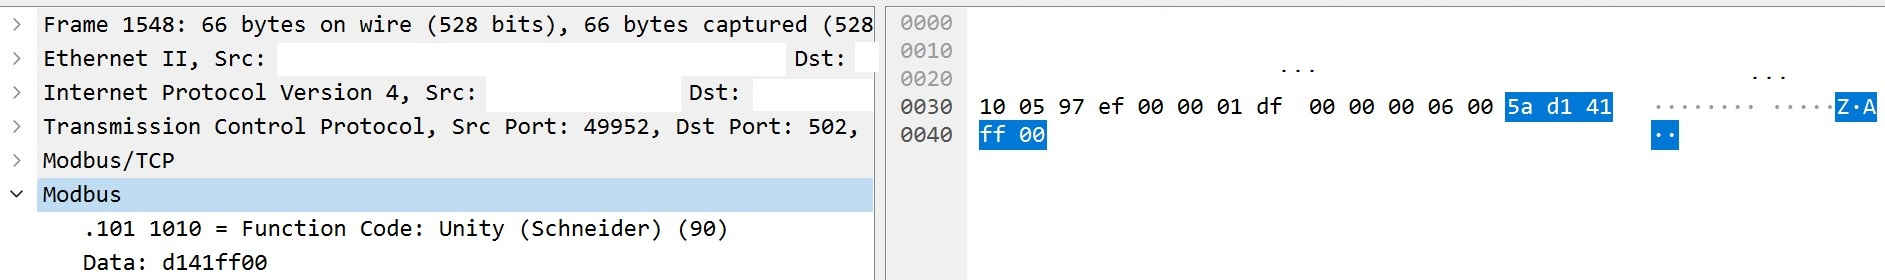
\includegraphics[width=\linewidth]{figures/plc-starts.jpg}
    \caption{Packet sent by the workstation to start the PLC.}
    \label{fig:start-plc}
\end{figure}

\subsubsection{Diagram Synthesis}

The synthesis diagram in~\autoref{fig:communication} models the connection establishment between the PLC and the workstation. After this connection, the engineering workstation sends to the PLC the command to start it. 

\subsection{Exploiting the ModiPwn Vulnerability}

The ModiPwn vulnerability (i.e., CVE-2021-22779~\cite{modipwn-cve-details}) crafts an authenticated packet by simply spoofing the communication. 

First, let \texttt{hw\_id} denotes the hardware identifier. This identifier is fixed and specific to the PLC. The PLC sends this identifier when the engineering workstation requests for it as show in~\autoref{fig:hw-id-packets}.

\begin{figure}[H]
    \centering
    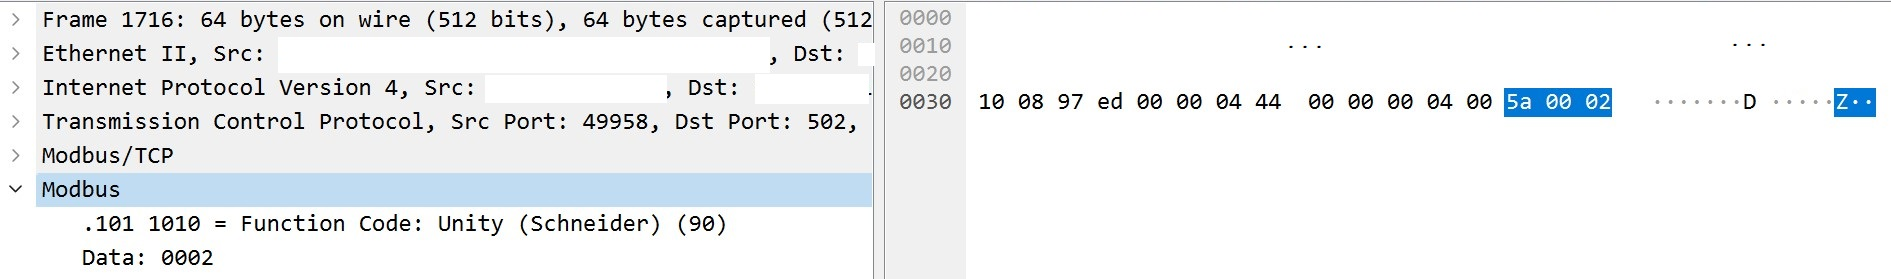
\includegraphics[width=\linewidth]{figures/ask-hw-id}
    \\ \vspace{1cm}
    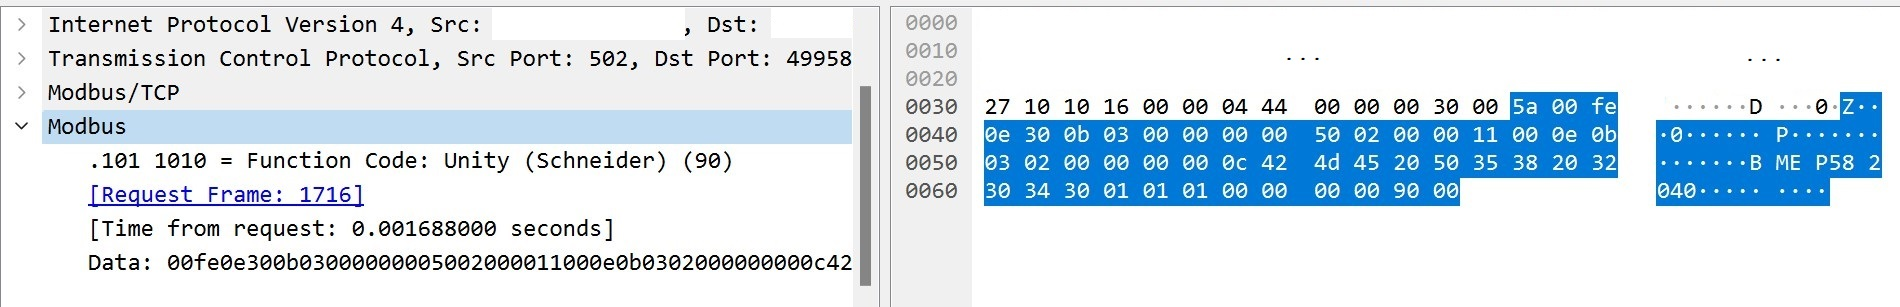
\includegraphics[width=\linewidth]{figures/send-hw-id}
    \caption{Top: Packet sent by the workstation to obtain the hardware identifier after connection establishment (i.e., request \texttt{0x02}). Bottom: Packet replied by the PLC with the hardware identifier (i.e., \texttt{0x0e0b0302}) and communication module name (i.e., \texttt{BMEP582040}).}
    \label{fig:hw-id-packets}
\end{figure}

A strong authenticated modbus command (e.g., start PLC) is composed as such : 

\noindent \texttt{0x5A}, \texttt{session}, \texttt{UMAS function code}, \texttt{SHA256(SHA256(hw\_id + client\_nonce) + \texttt{0x5A} + \texttt{session} + command + SHA256(hw\_id + server\_nonce))}, \texttt{command}. 

As an example, the command to start the PLC is \texttt{command = 0x40FF00}.

The ModiPwn vulnerability exploits the fact that all values (\texttt{session}, \texttt{hw\_id}, \texttt{client\_nonce}, \texttt{server\_nonce}) are known to an adversary only spoofing the communication. An adversary can thus craft any authenticated chosen-\texttt{command} packet. 

As an important note, a patient adversarial spoofer observing any authenticated packet could perform a replay attack. Indeed, the packet authentication does not prevent from a replay attack as the packets do not depend on a timestamp or a tagging mechanism.

\subsection{\texttt{MONITOR\_PLC}: Arbitrary Read/Write on PLC's System Bits or Words}

The UMAS communication protocol includes a \texttt{MONITOR\_PLC} function (\texttt{0x50}) to read or write system bits or words. To do so, first, the workstation must send a packet to inform which variables to monitor and then must send a second packet to read or write one variable. The \texttt{MONITOR\_PLC} packet takes the following format:

\noindent \texttt{0x5A}, \texttt{session}, \texttt{0x50 0x15 0x00 0x03 0x01}, \texttt{header}, \texttt{read/write}, \texttt{length}, \texttt{action} (read or write), \texttt{code}, \texttt{system bit}, \texttt{system bit to read/write + 4}, \texttt{unknown}, \texttt{system bit value to write} (if write), \texttt{0x00 0x00 0x00 0x01}

In short, the adversary needs to guess what is the system bit/word memory location. But, if the adversary has access to the program running on the PLC, it has access to this mapping and can thus read or write any wanted variable. For this reason the \emph{NinjaCrane} attack includes program exfiltration, requiring the workstation to be connected to the internet. Furthermore, the \emph{NinjaCrane} attack will then use this \texttt{MONITOR\_PLC} function to change the variable associated to the speed of the polar crane or to the activation of the polar crane rotation.
%%%%%%%%%%%%%%%%%%%%%%%%
\chapter{The NinjaCrane Attack}
% The implementation covers some of the implementation details of your project.
% This is not intended to be a low level description of every line of code that you wrote but covers the implementation aspects of the projects.
% This section is usually 3-5 pages.
%%%%%%%%%%%%%%%%%%%%%%%%
\label{chapter:ninja-crane-atk}

\section{Entry Points}

The implementation choice of the entry point infecting the workstation has been to create two equivalent entry points — the USB Ninja cable and the malicious mouse. Payloads stored on the USB Ninja cable can be triggered over BLE which makes it more interactive for a live demonstrator. The drawback of the USB Ninja cable is the storage capacity, too small to store the \emph{NinjaCrane} malware. The \emph{NinjaCrane} malware must be already downloaded or stored on the workstation (or on the device connected to this USB Ninja cable). To overcome this, a malicious mouse has been made. It offers a better flexibility as any board with USB-B connector can be placed and connected inside the mouse. This allows to store the malware directly inside the mouse.

\subsection{USB Ninja}

The BLE communication protocol used by the USB Ninja cable has been reverse-engineered by the Embedded Lab Vienna for IoT \& Security~\cite{ninja-cable-reverse}. From this work, a script controlling the USB Ninja cable from the BLE of a windows computer has been made with the help of the \texttt{bleak} python package.

Given the USB Ninja cable's Bluetooth MAC address, the script connects to its associated BLE GATT server. To trigger the payloads stored on the USB Ninja cable, two BLE packets are sent consecutively. The first one writes at BLE handle $\texttt{0x36}$ the password. The second packet writes at BLE handle $\texttt{0x36}$ either \texttt{A=L$\backslash$r$\backslash$n} or \texttt{B=L$\backslash$r$\backslash$n} to trigger the first or the second payload respectively. The script is used by the attacker's GUI; button \texttt{Deploy Payload} sends \texttt{A=L$\backslash$r$\backslash$n} and button \texttt{Trigger Attack A} sends \texttt{B=L$\backslash$r$\backslash$n} to the USB Ninja cable.

\subsection{Malicious Mouse}

The clean mouse is a Logitech M90 USB wired mouse. A DIY Tiny USB Hub~\cite{usb-diy-hub}, placed inside this mouse, splits the USB wired connection in order to connect both the mouse and a micro USB type-B male connector. A pre-programmed Adafruit Trinket M0 is plugged to this connector. The Trinket M0 is a HID-capable device that can emulate a keyboard or a mouse. Picture of this assembly can be found in~\autoref{fig:infected-mouse-photo}. The Trinket M0 is programmed using \href{https://circuitpython.org/}{\texttt{CircuitPython v8.2.0}} by placing in its associated USB drive two different files (\texttt{code.py} and \texttt{boot.py}). When the Trinket is plugged-in the \texttt{boot.py} and the \texttt{code.py} scripts are respectively executed. The first script will deactivate Midi, REPL and USB drive (but not HID). The second script executes the HID payload and then activates the USB drive where the malware is stored. 

\subsection{Payloads of the HID-capable Device}

The payload of the cable executes the following instructions: open Run command, open a hidden powershell terminal, write and execute a script that will detect internet connection, download a malware and execute it in background. Moreover, for a background persistence, a malware's shortcut is placed in the engineering workstation startup folder.

The payload of the mouse executes similar instructions: open Run command, open a hidden powershell terminal, and execute the malware in background. No internet connection is required as the malware is stored in the malicious mouse.


\section{Attacker's GUI}

No attacker's GUI are available to control the malicious mouse as the Trinket M0 has no wireless communication. But if the entry point is the USB Ninja cable, a python interface to control the attack can be used. This interface is shown in~\autoref{fig:gui}. Python interface has been written with \emph{PySimpleGUI} package in order to better illustrate the steps taken by adversary and simplify the attack explanations. This GUI is made of one interface modeling the attack progress on the ICS architecture and two buttons. The first button \texttt{Deploy Payload} will trigger the first payload stored on the USB Ninja cable. The second button \texttt{Trigger Attack A} will trigger the second payload stored on the USB cable.

\section{The \emph{NinjaCrane} Malware}

The \emph{NinjaCrane} malware is a python script that is converted into an executable file named \texttt{malwar3.exe}.

\subsection{MITM Script}

The MITM script is a .pyw extension python file for better flexibility and stealthiness. This script first by-pass the UAC consent prompt to execute itself with admin rights. It then waits for a trigger to perform the MITM attack on the polar crane.

\subsubsection{UAC Consent Prompt By-Passing}

First, the script detects if it runs with administrative privilege. If not it will exploit the \texttt{fodhelper.exe} weakness (i.e., \texttt{fodhelper.exe} elevates itself to run in a higher integrity level) to execute again itself with admin privilege. Otherwise it continues with the attack. 

To exploit the \texttt{fodhelper.exe} weakness, two register keys are created at \texttt{HKEY\_CURRENT\_USER$\backslash$Software$\backslash$Classes$\backslash$ms-settings$\backslash$shell$\backslash$open$\backslash$command}. The first key (\texttt{DelegateExecute}) is set to empty string and the second key (Nil) is set to the command to execute with higher integrity context (i.e., executes this python script again) as shown in~\autoref{fig:reg-uas-bypass}. No privilege are needed to modify and create those \texttt{HKEY\_CURRENT\_USER} register keys. Finally, the python script executes \texttt{C:$\backslash$$\backslash$Windows$\backslash$$\backslash$System32$\backslash$$\backslash$fodhelper.exe} to run itself again with higher privilege. 

\begin{figure}[H]
    \centering
    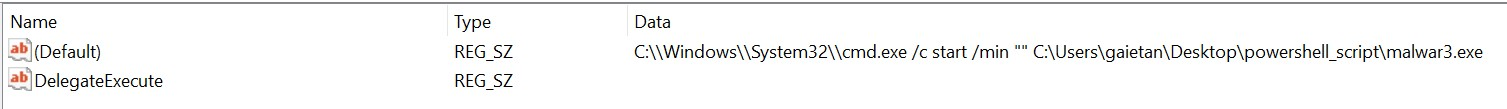
\includegraphics[width=\linewidth]{figures/reg-uac-bypass.jpg}
    \caption{Register keys created to By-Pass Windows Consent Prompt UAC}
    \label{fig:reg-uas-bypass}
\end{figure}

\subsubsection{Waiting for Attack Trigger}

Once the script executes with admin privilege it makes use of the \texttt{pydivert} package to listen and modify the packets sent by the workstation to the PLC. The \texttt{pydivert} package is itself based on Windows Packet Divert (named \texttt{WinDivert}), a capture-and-divert package for Windows. 

The script captures only the UMAS packets (i.e. packets from/to the engineering workstation's $503$ TCP port). The script extracts the key information e.g., \texttt{server\_nonce}, \texttt{client\_nonce}, \texttt{salts} \& \texttt{hash}, Unity Pro version, project name, project folder etc. 

\subsubsection{Data Exfiltration}

As soon as the script extracts the project folder it will try to exfiltrate over internet the\texttt{.STU} program and a text file with project information. The text file with project information is stored in the \texttt{$\backslash$Desktop$\backslash$powershell\_script$\backslash$extracted\_info.txt}. The script thus uploads from the workstation the two files on a \href{transfer.sh}{\texttt{transfer.sh}} server and sends an SMTP email with the corresponding urls with the use of the \href{https://mailtrap.io/}{\texttt{mailtrap}} solution. The attacker from outside, receiving this email can then download those two files as shown in~\autoref{fig:mailtrap-exfiltrate-data}.

This data exfiltration allows the adversary to perform aside an analysis of the .STU program running on the PLC and to better weaponize the malware. Indeed, as soon as the adversary has access to the program, it has access to the memory addresses of every variables, their use and their type. This allows the adversary to craft a valid authenticated packet to modify or read any of those variables. 

\subsubsection{Send Malicious Authenticated Packet}

\label{subsec:malicious-sent-packets}

When the adversary triggers the attack (or when mouse is plugged-in), the USB Ninja (or malicious mouse respectively) will write to a text file. The script is continuously reading this text file. In case of file modification, the script will start to send malicious authenticated packets. For a better cyberattack illustration purpose the following malicious packets are sent:

\begin{itemize}
    \item \textbf{Packet 1}: Sends a request to initiate the variables monitoring.
    \item \textbf{Packet 2}: Sets the rotation speed of the polar crane's rotation to 34 \% of the maximum motor's speed. 
    \item \textbf{Packet 3 \& 4}: Activate the polar crane's rotation. First is a rising edge (i.e., sets the corresponding internal variable to 1) the other one is a falling edge (i.e., sets the corresponding internal variable to 0).
    \item \textbf{Packet 5}:  Sets the rotation speed of the polar crane's rotation to 63 \% of the maximum motor's speed. 
    \item \textbf{Packet 6 \& 7}: Activate the polar crane's rotation. Those packets are needed in order for the polar crane to apply the previously set rotation speed.
    \item \textbf{Packet 8 \& 9}: Deactivate rotation. First is a rising edge,  the other one is a falling edge.
    \item \textbf{Packet 10}: Stops the PLC.
\end{itemize}

To sum up, the above packets will make the polar crane rotate slowly first, then fast, then completely stop the polar crane and the PLC. This scenario could be improved to also show that the attacker can extract the value of the internal variables. To send the malicious packet the script completely modifies a sent \texttt{MONTOR\_PLC} (i.e., \texttt{0x50}) packet with the corresponding Modbus data. \texttt{PyDivert} automatically recomputes the checksum. However the TCP sequence and acknowledgment numbers must be modified according to the modified packet length. This modification must apply to any fresh packet sent or received (i.e., the script synchronizes the ack and seq numbers in order to avoid duplicate ack/seq, TCP re-transmission, and connection loss).

\subsection{Converting a Python Script to an Executable \emph{Malwar3.exe}}

As the engineering workstation has no python environment the script must be compiled. To compile the python script in one file, the \texttt{pyinstaller} package (or its Graphical Interface equivalent, \texttt{auto-py-to-exe 2.36.0}) has been used. Moreover the Ultimate Packer for eXecutables (UPX) reduces the compiled binary's size. The executed command to compile the python script is: \texttt{pyinstaller --noconfirm --onefile --windowed --upx-dir "path/to/upx\_filr"  "path/to/malware\_script.pyw"}
%%%%%%%%%%%%%%%%%%%%
\chapter{Evaluation}
% In the evaluation you convince the reader that your design works as intended.
% Describe the evaluation setup, the designed experiments, and how the experiments showcase the individual points you want to prove.
% This section is usually 5-10 pages.
%%%%%%%%%%%%%%%%%%%%
\label{chapter:evaluation}

\section{Raising Awareness with an Attack Demonstrator}

Demonstration video of the polar crane's cyberattack can be found in the \emph{NinjaCrane github}~\cite{MyGithub}. In parallel to this video a demonstration show has been created to better illustrate a real-world scenario and is detailed is the section.

\subsection{Demonstration Setup}

Two persons will act in the demonstration. The first plays the role of the polar crane's automation technician that programs the PLC with the use of his engineering workstation. The second one plays the role of the hacker. For simplicity, we assume that the hacker is in the same room as the technician. This is a violation with respect to the threat model (as a external adversary was assumed). The attacker can for example be a subcontractor. Finally the entry point used in this demonstrator is the USB Ninja cable (and not the malicious mouse).

The situation setup is the attacker talking with the technician and asking him to charge his phone (or any USB device) with the USB Ninja cable. The technician plugs the USB Ninja cable to charge his phone as shown in~\autoref{fig:plug-usb-cable}.

\begin{figure}[H]
    \centering
    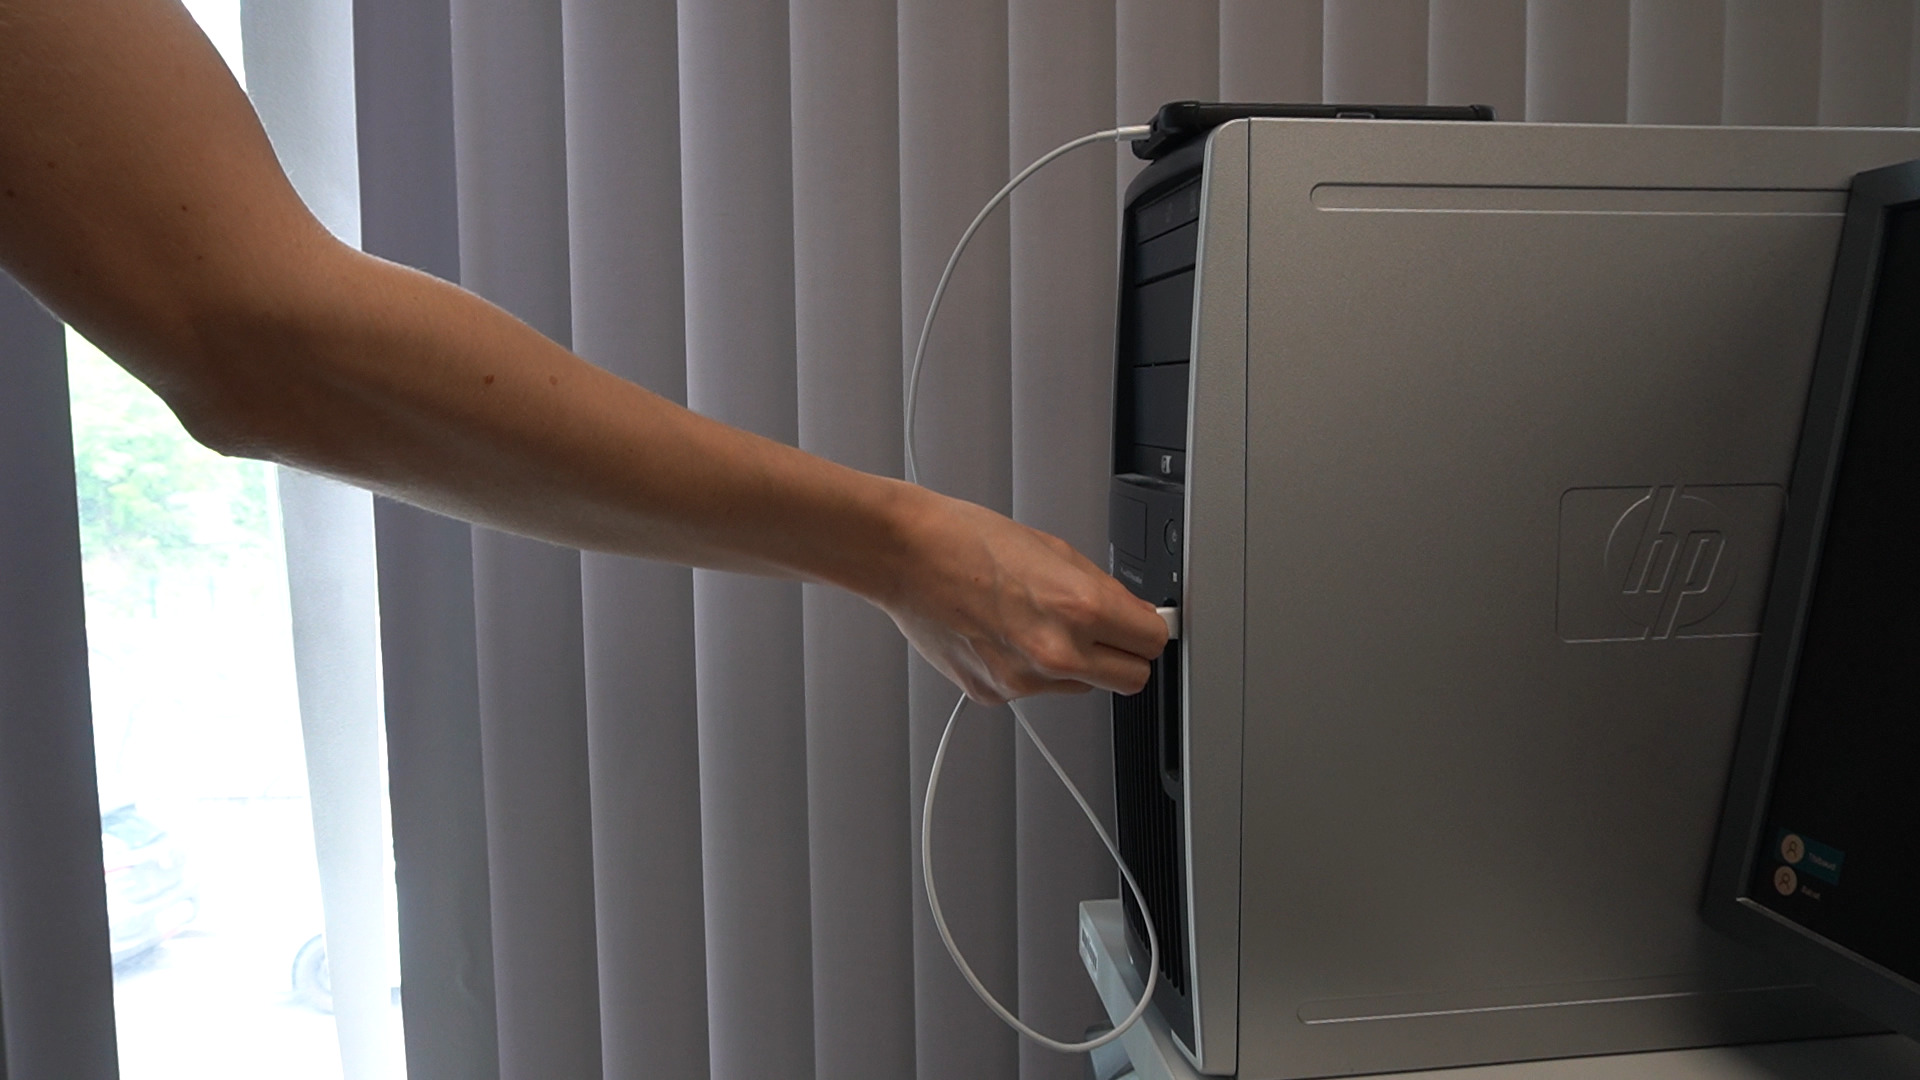
\includegraphics[trim={12cm 0 5cm 0}, clip, width=0.6\linewidth]{figures/plug-cable.jpg}
    \caption{Plugging USB Ninja Cable.}
    \label{fig:plug-usb-cable}
\end{figure}

\subsection{Engineering Workstation Infection}

Once the USB Ninja is plugged-in. The attacker will for example ask the technician to take a coffee break while leaving the session unlocked. Once done, the attacker triggers the USB Ninja cable with the adversary's GUI to run the payload. This will open the Execute service and open a powershell command in background to run the commands as shown in~\autoref{fig:execute}.

\begin{figure}[H]
    \centering
    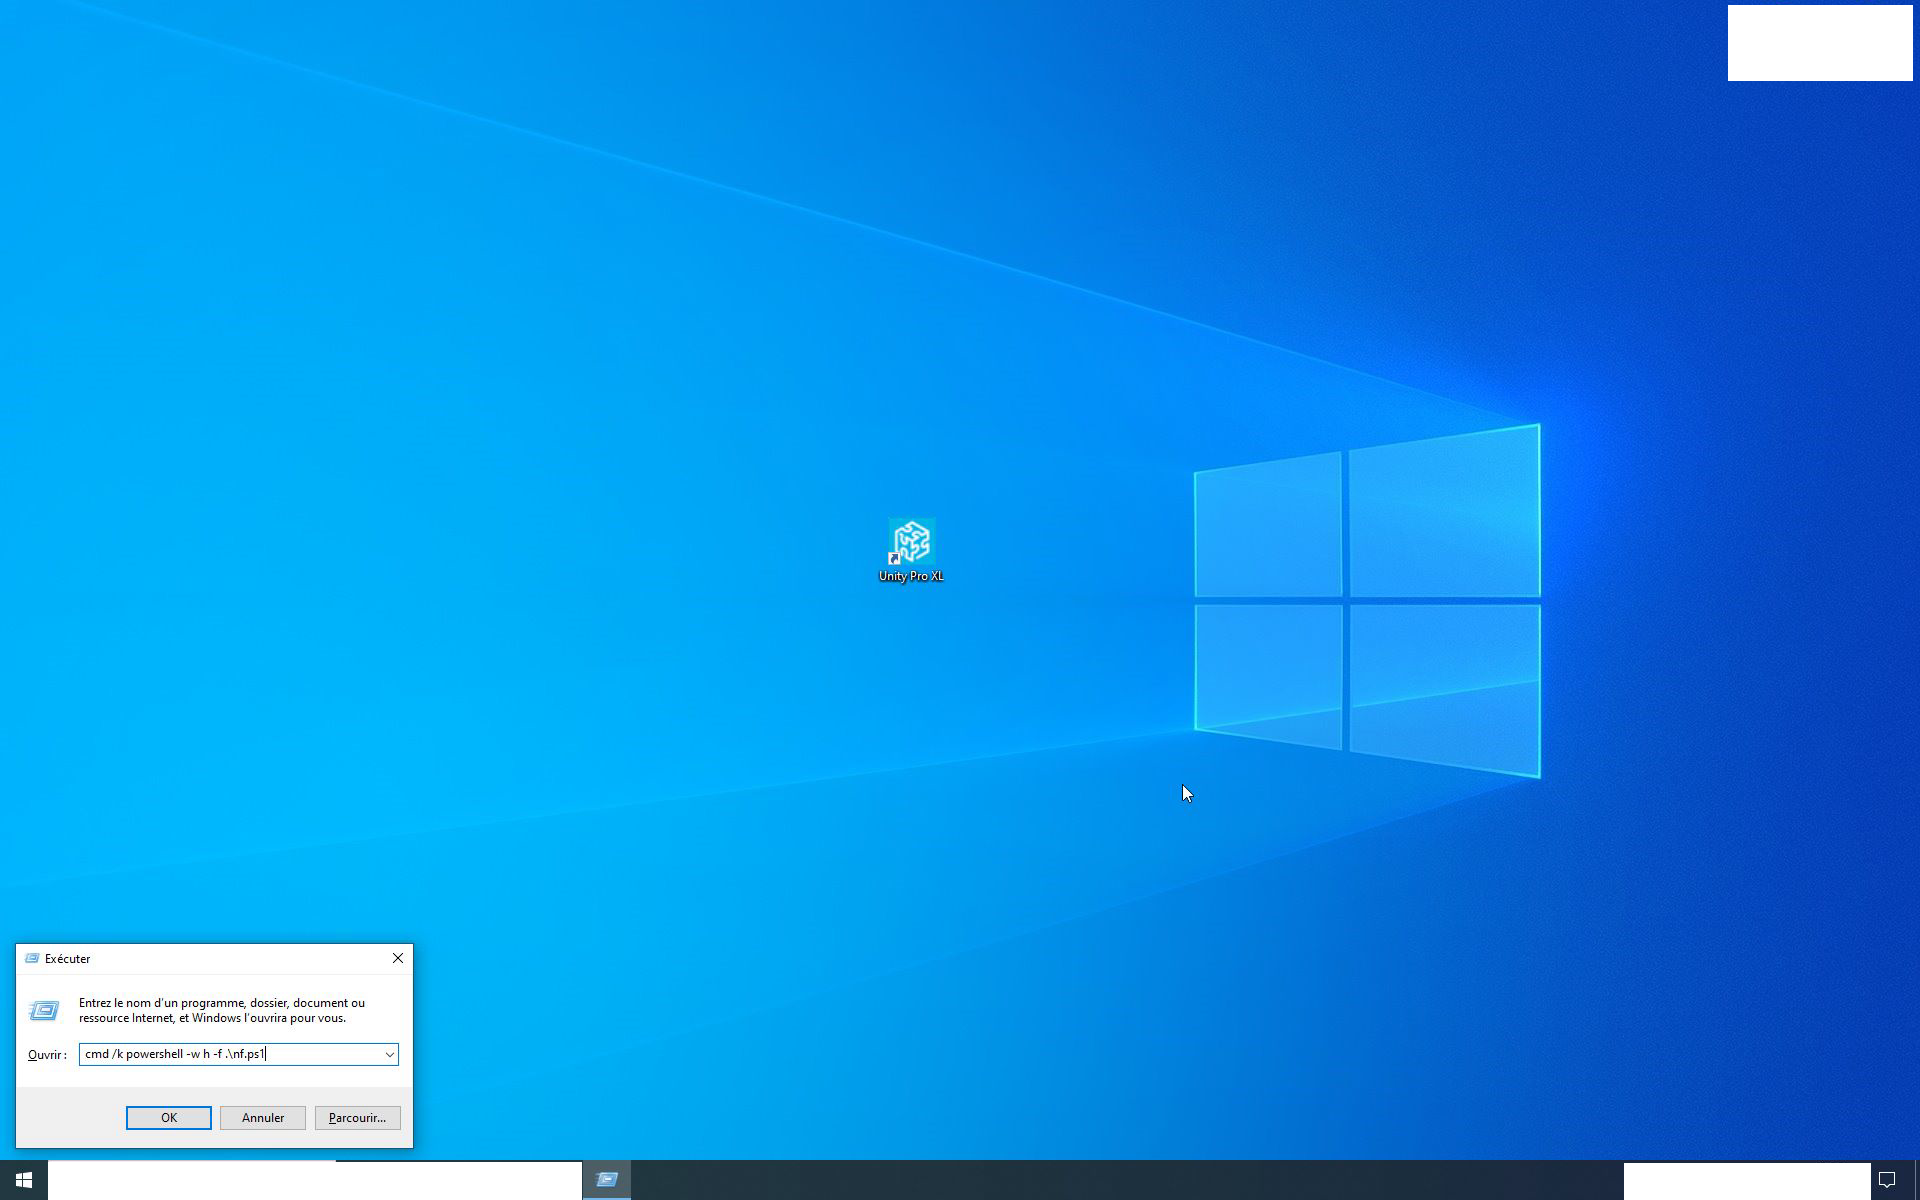
\includegraphics[trim={0cm 0cm 25cm 15cm}, clip, width=0.5\linewidth]{figures/execute.png}
    \caption{Opens the Execute service and opens a hidden powershell on the engineering workstation.}
    \label{fig:execute}
\end{figure}


The commands will create four files; \texttt{VBs.vbs} and \texttt{script.ps1} are scripts to download the malware and run it in background at each session opening, \texttt{malwar3.exe} is the downloaded \emph{NinjaCrane} malware performing the MITM attack and finally \texttt{trigger.txt} is the text file containing the instruction to triggers the polar crane's attack. The four files are created in the \texttt{Desktop/powershell\_script} folder as shown in~\autoref{fig:folder}. The~\autoref{fig:logigram} is a flowchart describing the sequence to infect to engineering workstation. For the demonstration, a modified version of the commands can be used to have an offline scenario that assumes that the \texttt{malwar3.exe} is already located at \texttt{$\backslash$Desktop$\backslash$Malware$\backslash$malwar3.exe}

\begin{figure}[H]
    \centering
    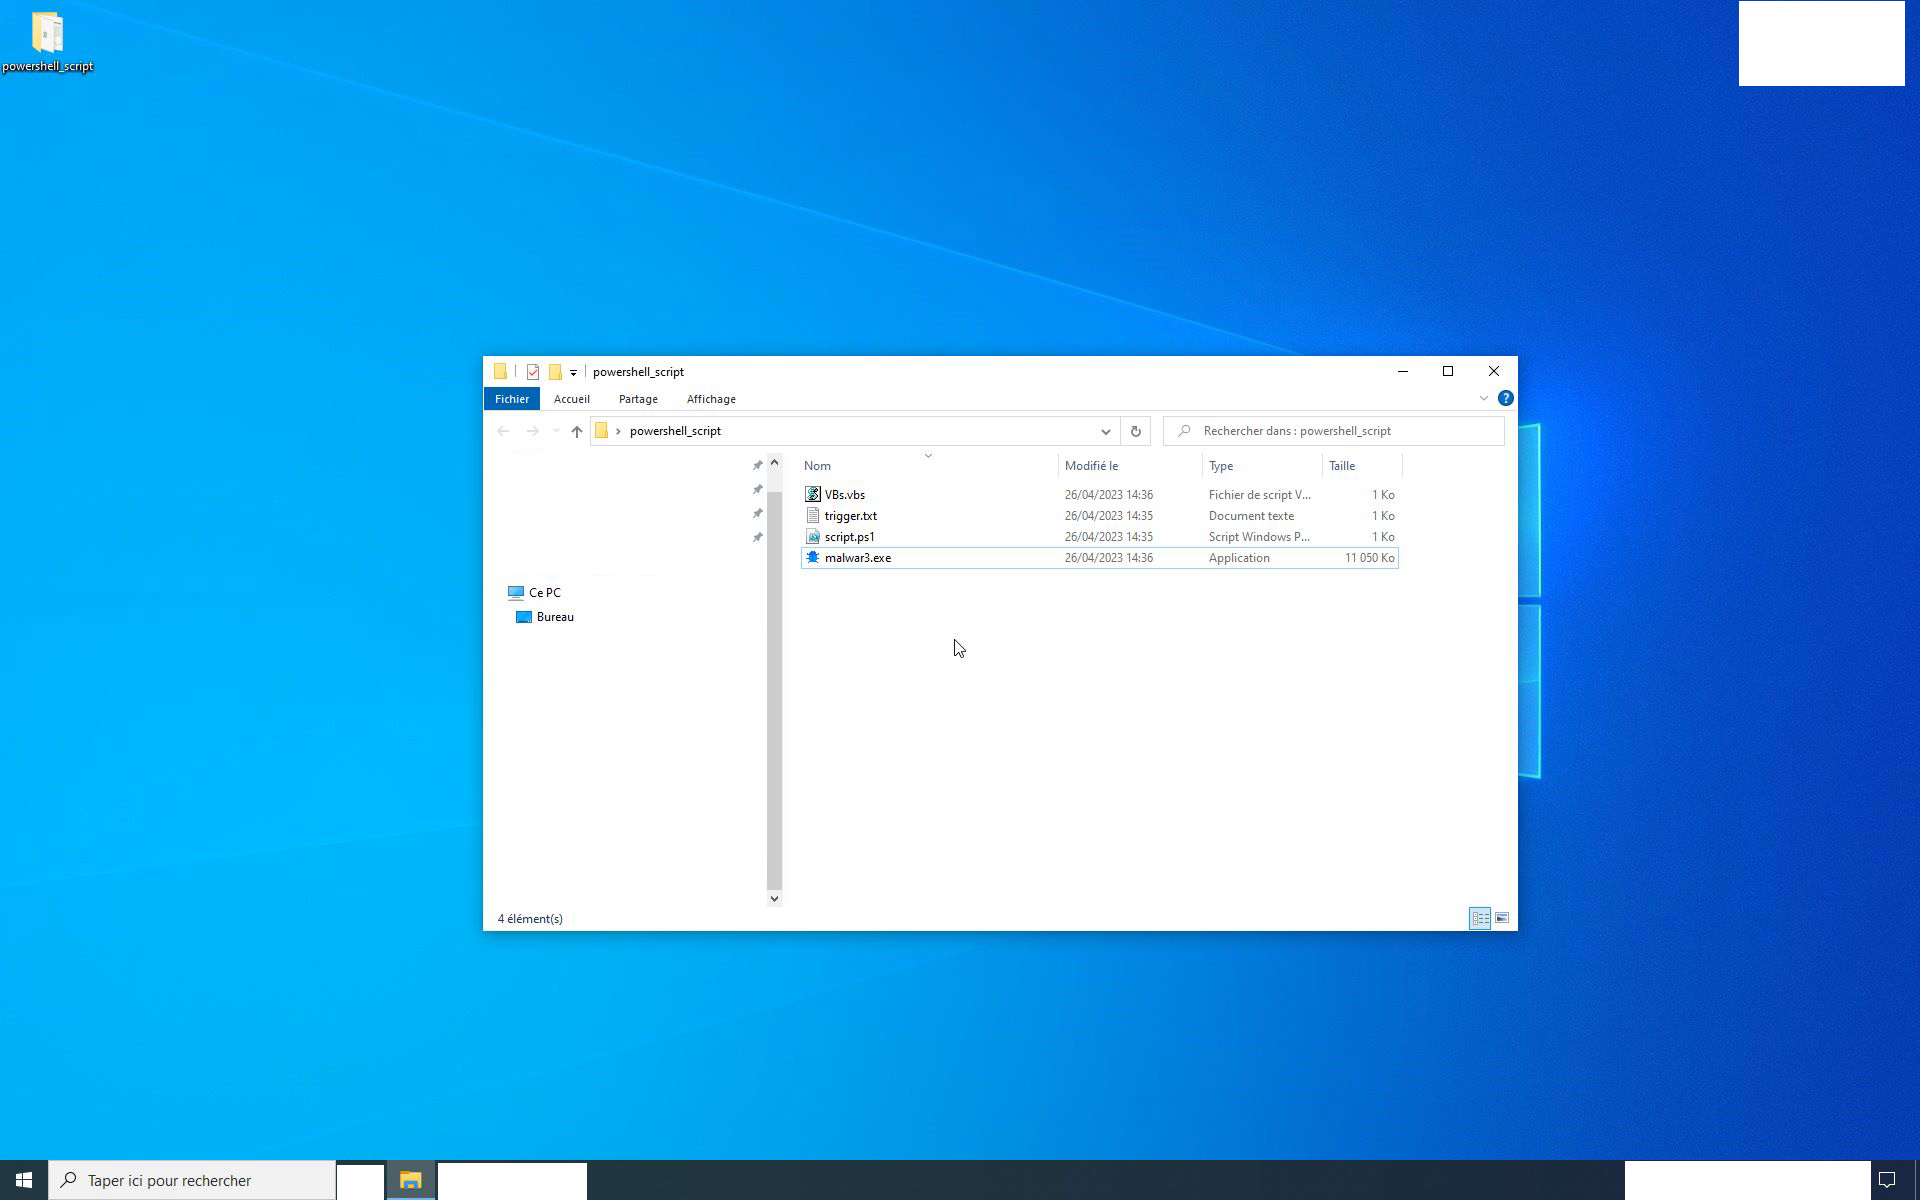
\includegraphics[trim={8cm 10cm 10cm 6cm}, clip, width=0.8\linewidth]{figures/folder.png}
    \caption{Created folders after the first USB Ninja payload execution.}
    \label{fig:folder}
\end{figure}

\subsection{Take the Polar Crane's Control}

Once the malware is running on the engineering workstation, the attacker triggers once again the USB Ninja cable to effectively disturb the polar crane as described in~\autoref{subsec:malicious-sent-packets}. The malware sends a packet to rotate the polar crane at 34\% of maximum speed then at 63\% of the maximum speed. This shows that the adversary could wear and tear the motor. Then it stops both the polar crane and the PLC. This shows that the adversary can stop the process at any time and for example stop the loaded polar crane above the reactor vessel. 

\begin{figure}[H]
    \centering
    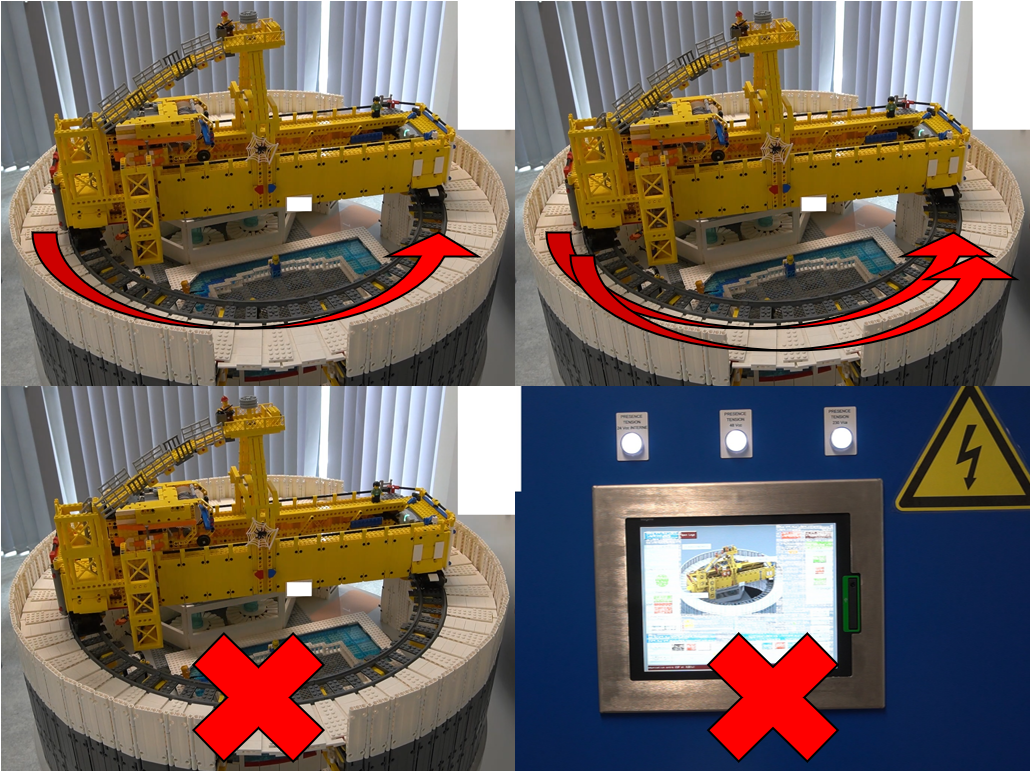
\includegraphics[width=0.9\linewidth]{figures/step-atk}
    \caption{Attack Sequence order from left to right. Top-Left: Make the polar crane rotates at 43\% of maximum speed. Top-Right: Make the polar crane rotates at higher speed (63\% of maximum speed). Bottom-Left: Stop the polar crane. Bottom-Right: Stop the PLC.}
    \label{fig:atk-steps}
\end{figure}

\section{Real World Feasibility of the Cyberattack}

\subsection{Engineering Workstation Infection}

Several observations can be made regarding the success of the engineering workstation infection.

\begin{itemize}
    \item Avast antivirus does not detect the malware executable as a threat. However, the avast antivirus fixed at a high protection level will notify the execution of the executable and ask the administrative user to block or not the execution. Moreover, the malware requires administrative privilege to execute. Thanks to the UAC bypassing method, it only requires that current logged-in user has administrative right and that the UAC level is not set to "Always Notify". 
    \item There must be no protection regarding HID-capable device. Since July 2021, the Windows environment has a built-in solution to restrict USB devices called Microsoft Intune~\cite{intune-servie},~\cite{introduce-grp-policy}. The Intune service is a system policy that blocks any USB device not matching the hardware ID whitelist given by the user.
    \item HID-based attacks come with major drawbacks. First, an event must trigger the attack. It can be a time-based event (e.g., keyboard frames are sent 10 seconds after the connection) or attacker-based event (e.g., attacker triggers the attack over BLE, as for the USB Ninja). Moreover, if windows password account is unknown to the adversary, this trigger must be run during a session unlocked. And if windows password is known to the adversary, the workstation must be turned-on. Finally, as the payload is made of keyboard frames, the attack is not completely stealth during few seconds — the time to type all the key-frames. 
\end{itemize}

\subsection{Live Demonstration Feedback}

This demonstration has been played during the \emph{Journée Sûreté} at the \emph{Direction Projet Nouveau Nucléaire }, during the \emph{Plénière} of the \emph{Département des Composants Electriques et Electromécaniques} and partially-played (i.e., only with a video support) at the \emph{Cercle d'Experts Sûrté sur la Cybersécurté} at \emph{EDF Saclay}. The demos were played with the goal to raise awareness on cybersecurity and to show how a malware could propagate from the IT to the OT systems in case of security policy breach. The demo shows a concrete social engineering scenario that leads to the industrial process failure  — the polar crane stops as well as the connection between the workstation and the PLC. Anonymously collected feedback from the demo participants can be find in~\autoref{annex:feedback}. One downside regarding the reliability of the demo can be noted. Indeed, the connection between the PLC and the engineering workstation can sometimes drop due to time-out or the engineering workstation infection must sometimes be repeated in case of bluetooth connection lost with the USB Ninja cable or if a mouse click is made during the HID-keystrokes injection.


\subsection{MITM Malware Attack}

Similarly, some observations can be made regarding the success of the MITM attack.

\begin{itemize}
    \item The MITM malware must catch the connection phase with the PLC to conduct later the attack phase. Moreover during the attack phase, engineering workstation and PLC must be connected. Unfortunately, due to connection time-out the connection between the workstation and the PLC may drop after half an hour. To overcome this, the timeout variable in Unity Pro can be increased. 
    
    \item In the current state, the \emph{NinjaCrane} attack is not resilient to program change that results in the change of variable memory location. Indeed, the attack crafts and sends pre-fixed packet to change the value of a specific memory location corresponding to a PLC's inner variable. 

    \item The attack sequence played by \emph{NinjaCrane} malware is fixed and does not consider the current state of the polar crane. During the demonstration, \emph{NinjaCrane} malware assumes that the polar crane's and PLC are already in a specific state (i.e., PLC is in run and is in the mode to control the polar crane). However, this might not be the case and the \emph{NinjaCrane} malware needs to be adjusted accordingly. For example the \emph{NinjaCrane} malware could craft some packets to read some variable states or could be made reactive by adjusting the sent packet according to the information previously gathered by observing the communication.
\end{itemize}

\section{Mitigation and Counter Measures}

\subsection{Engineering Workstation Hardening}

Solutions for engineering workstation hardening are highly-dependent on the use-case, environment, and threat model. Below is a non-exhaustive list of solutions that would have blocked the \emph{NinjaCrane} attack:

\begin{itemize}
    \item Physically blocking the USB port (e.g., Lindy USB Port Blocker). It physically prevents the use of the USB port. However the blocker can be forced and the key to unlock the blocker is any-blocker compatible.
    \item Physically blocking the data transfer wires (e.g., USB Condom). The data blocker physically prevents any data transfer but can still be used for slow charging. Charge-only cables also exist. ~\autoref{fig:data_blocker} illustrates physically how the USB data blocker works.
    \begin{figure}[H]
        \centering
        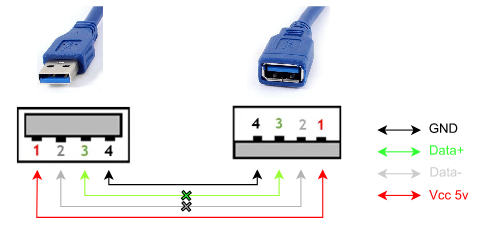
\includegraphics[height=4cm]{figures/data-blocker.png}
        \caption{Data blocker. The data blocker cuts the Data+ and Data- transmission.}
        \label{fig:data_blocker}
    \end{figure}
    \item De-activates USB port. This could be done via the BIOS, via Group Policy, Device Manager, 3rd party software, or uninstalling the USB driver.
    \item De-activates USB port based on whitelisting. This can be setup via Microsoft Intune, Group Policy or 3rd party software. USB ID device can however easily be spoofed. 
    \item \emph{USBFILTER} solution from Tian et al.~\cite{Tian15}~\cite{tian16} (or similarly \emph{Netfilter}) instruments the USB stack to filter USB packets at a fine granularity following user-defined rules. With correct rules, this solution prevents a mouse or a charging cable to act as a keyboard. Similarly the \emph{GoodUSB} solution  (currently only available for the Linux USB Stack) associate user's expectation of the device's functionality.
\end{itemize}


\subsection{Cybersecurity of the Supply Chain}

Cybersecurity over the Supply Chain is still in active development and mostly boils down to the cybersecurity principles — separation and least privilege, monitoring, life cycle development (e.g., V model), access controls, audits and regular security assessments, sensitive data encryption etc. Below is a non-exhaustive list of practical solutions that would have blocked the \emph{NinjaCrane} attack:

\begin{itemize}
    \item Blockchain technology (e.g., VeChain or ChainLink). Blockchain can help to ensure products authenticity, movements and origins via tamper-proof records available to the supply chain tenants. 
    \item In-depth inspection. Inspection can take the form of randomized security assessments of the electronic devices. By opening the maliciously tampered mouse or the USB Ninja cable the alteration would have been detected. Furthermore, characteristics inspection would also be a working lead (e.g., mouse weight or USB Ninja cable heating).
    \item Strict security policy between the tenants of the supply chain. As an example, the USB Ninja cable could be offered to an employee as a gift.
\end{itemize}

%%%%%%%%%%%%%%%%%%%%%%
\chapter{Related Work}
% The related work section covers closely related work. Here you can highlight the related work, how it solved the problem, and why it solved a different problem. Do not play down the importance of related work, all of these systems have been published and evaluated! Say what is different and how you overcome some of the weaknesses of related work by discussing the  trade-offs. Stay positive!

% This section is usually 3-5 pages.
%%%%%%%%%%%%%%%%%%%%%%

In this chapter is described the closely related work, without any attempt to compile an exhaustive list. 
In the MSc thesis was developed an APT attack on a non-simulated NPP-related process testbed. Most of the literature is based either on process simulation or on system virtualization. First section describes some cyberattack demonstrators or testbeds of ICS based on virtualization or on a hybrid configuration (called Hardware-In-The-Loop) of software-virtualization and hardware. They offer better flexibility, lower cost, better portability but suffer from a lack of representativeness compared to this study. Second section focuses on related work that includes non-simulated industrial process.

\section{Hardware-In-The-Loop-based or Virtualized Attack Demonstrator on ICS Based on Simulated Industrial Process}

De Brito et al.~\cite{deBrito22} built a Modbus/TCP network testbed simulating the NPP process (with Asherah NPP Simulator) and including a SCADA system (ScadaBR), a rogue PLC (OpenPLC on Arduino), an inside adversary (Kali Linux system), and a historian. The proposed cyberattack assumes that the adversary already neutralized a control system and replaced it by a rogue PLC. The rogue PLC maliciously tampers a pump speed variable while the Kali Linux system conducts a MITM attack so that the SCADA does not notice this tampering. De Brito et al. also explored a network monitoring defense based on the "Time from request".  This work proposes a low-cost, simplified, and hybrid network testbed to conduct cyberattack on an ICS of a NPP. As this Master thesis, a MITM attack on Modbus/TCP is conducted, however the adversary is assumed to be inside the network with a Kali Linux system and a rogue PLC and adversary directly targets the NPP process. 

Puys et al.~\cite{puys21} proposed two Hardware-In-The-Loop cyber-ranges in order to build an ICS cybersecurity awareness and a student training program respectively. First one, WonderICS, includes 3D simulation of an industrial process (i.e., hazardous gases management, hydroelectric power plant, chemical process of Tennessee-Eastman), PLCs, protection relay,  HMIs, Kali Linux Virtual Machine (VM), engineering workstation VM. Two attack scenarios were considered but the first one is the closest to the attack presented in this MSc project. It makes use of a Rubber Ducky USB key that performs cryptolocking, keyboard disabling, and PLC commands injection. The attack injects a malicious Modbus frame writing a fake value on the PLC's register. In comparison to the \emph{NinjaCrane} attack, it offers less stealthiness - a malicious cable or mouse is more stealth than a Rubber Ducky - and no flexibility - as the charge delivery and exploitation are automatically and instantaneously launching when Rubber Ducky is plugged-in. The second HIL cyber-range is called G-ICS and it offers a student training program. The students can then practice malicious packet injection, firewall rule editing (to protect against a known exploit), industrial proprietary protocols reverse-engineering and protocol fuzzing to find a protocol vulnerability.

Much research have been made to construct an ICS testbed for cybersecurity training such as the KYPO4INDUSTRY~\cite{celeda20}, the Micro-CI Testbed from Hurst et al.~\cite{ljmu5763}, or the EPS-ICS Testbed from Gao et al.\cite{Gao13}. None of them includes an APT scenario, however they all propose a flexible, pedagogical, portable and low-cost solution.

\section{Cybersecurity Testbed on ICS Based on Non-simulated Industrial Process}

Several universities have developed more realistic industrial processes such as Technische Hochschule Augsburg with LICSTER~\cite{Sauer19}. LICSTER is a simple open-source and low-cost ICS testbed where several single step attacks at any ICS level can be conducted such as sniffing, DoS or MITM. It benefits from its simplicity while still proposing a haptic understanding of the consequences of the cyberattack on the ICS. The testbed includes open-source Remote IO, PLC, SCADA and HMI. 

The New Orleans University SCADA testbed from Ahmed et al.~\cite{Ahmed16} includes three (simulated and non-simulated) industrial processes. It is made of PLC, Relay, switch, historian and HMI. Even though no cyberattack has been made it offers diversity, with the presence of three different vendors PLC to reverse-engineer the proprietary communication protocols.

A practical cyberattack demonstrator has also been made by \emph{Bristol Cyber Security Group}~\cite{Gardiner19}~\cite{Craggs19}~\cite{Rashid20}, where A. Rashid et al. created a full attack scenario starting from cloud IoT infrastructure and causing at the end water treatment process enter into an unsafe state. They exploited \emph{Tomcat} vulnerabilities, malicious PDF and a zero-day \emph{SCADAPack} vulnerability. This testbed illustrates how complex an attack in several steps can be made. The attacker is still assumed to be inside the SCADA network but A. Rashid et al. suggest that a malicious USB device could be the attack vector. This ICS training testbed including an APT scenario is believed to be the most advanced one and realist in the literature. In comparison, the \emph{NinjaCrane} attack can be seen as another APT scenario that reinforces the need to monitor the supply chain and the need to integrate cryptographic authentication standard in the industrial proprietary protocol. 

This need to have a better fidelity in the industry field pushed companies to build their own ICS testbed like the OPSWAT (CIP Lab) electric station ICS~\cite{opswat22} or the \emph{Check Point} chemical plant ICS testbed~\cite{checkpoint2023}. \emph{OPSWAT} (i.e. \emph{CIP Lab}) built an electric station ICS to promote their \emph{OTfuse} defense solution~\cite{opswat22}. The second testbed, the \emph{Check Point 1200R} security gateway is connected to the ICS network and prevents part of the fuzzing attacks, value-tampering attacks or exploitation of known vulnerabilities. This work is focusing on the ICS defense and not on the attack exploration nor the awareness part unlike presented work. As a side observation, the \emph{NinjaCrane} attack exploiting the \emph{ModiPwn} vulnerability would not have been detected by their security gateway.


%%%%%%%%%%%%%%%%%%%%
\chapter{Conclusion}
% In the conclusion you repeat the main result and finalize the discussion of your project. Mention the core results and why as well as how your system advances the status quo.
%%%%%%%%%%%%%%%%%%%%

\section{Future Work}

The major drawbacks of HID-based attacks, like the malicious mouse or cable, is the need to perform the attack while the workstation is on and session is unlocked — if windows account password is unknown to the attacker. This generally only happens when the workstation is in use. Moreover, as the attack emulates keystrokes, it is never completely stealth and a window flashes on the computer. The moment to trigger the HID payload plays a key role to conduct a stealth attack. It is generally triggered using a timer, over WiFi, or over BLE as in this study. In order to perform the HID-based attack while the session is locked — and windows account password is unknown — a maliciously modified keyboard spoofing the password (i.e., hardware key-logger) and then performing the HID-based attack can be considered. This can be done by modifying the electrical schematic from~\autoref{fig:infected-mouse-wiring} by replacing the mouse by a keyboard and adding a spliced GPIO-to-USB converter that transmits the sent keystrokes from keyboard to the Trinket M0. Alternatively, other USB attacks can be considered with stealth auto-run capability (e.g.,  LNK stuxnet/fanny USB flash drive exploit,  AutoRun exploits, Buffer overflow based attack etc.) and apparition of a fake lock-screen to spoof the windows password (see \emph{NinjaCrane github}~\cite{MyGithub}) for privilege escalation. 

The malware performing the MITM attack is a heavy executable (around 11 Mo) due to the fact that it is a python converted script and can thus not be stored on a microcontroller Read Only Memory (ROM). To overcome this, the malware could be re-written in low level language with the help of \texttt{WinDivert}~\cite{windivert}. 

Moreover, a third point to be improve is the need to run the malware with admin privilege. The malware can bypass UAC consent prompt but it requires that the current logged-in user has admin privilege. To relax this assumption, windows privilege escalation technique must be used like the \texttt{winPEAS} solution~\cite{winpeass} working on previous Windows versions. As an observation, the engineering workstation is rarely connected to the internet and the non updated workstation assumption might be added in the threat model.

The polar crane testbed offers an ideal environment to study the UMAS protocol and to explore fuzzing techniques on the PLC like boofuzz or mutiny fuzz~\cite{Gao21}. Furthermore the \emph{NinjaCrane} attack is a first stage to explore the defense mechanisms to protect for example against USB attacks. The \emph{Microsoft Intune}~\cite{intune-servie} solution is not a silver bullet as it raises problems about maintaining the HID whitelist and it does not protect against all USB-based attacks. Other software-based solution could be integrated as the integrity system from Griscioli et al.~\cite{Griscioli16} making use of cryptographic primitives (but not preventing HID-based attack), the \emph{GoodUSB} or the \emph{USBFILTER} solution from Tian et al.~\cite{Tian15}~\cite{tian16} trying to protect the USB stack or to add a USB firewall respectively. 

 

\section{Conclusion}

This study developed a cybersecurity attack demonstrator called \emph{NinjaCrane} on the polar crane's ICS. The \emph{NinjaCrane} attack is the first cyberattack demonstrator in the literature targeting a specific nuclear equipment of a NPP — the polar crane. The polar crane is a handling equipment situated in the CB and used during nuclear unit shutdown to carry and move heavy loads. By targeting a non-simulated PLC controlling the polar crane, the \emph{NinjaCrane} offers a framework for an awareness program on OT cybersecurity with high realism level.

The \emph{NinjaCrane} attack first infects the engineering workstation in the air-gap polar crane's ICS via the connection of a malicious USB device — a malicious mouse or a malicious USB Ninja cable — on this network. It then executes a persistent malware performing data exfiltration and lateral movement. Regarding data exfiltration, the malware running on the engineering workstation will send an email if it is connected to the internet with the control logic program and some PLC and workstation information. Regarding lateral movement, the malware performs a MITM attack to write arbitrary system bits in the PLC and take the control of the polar crane process. By taking control over the polar crane's ICS it is possible to create a significant safety event — a load stuck above the reactor pressure vessel.

The \emph{NinjaCrane} attack highlights the importance to monitor the USB-capable devices brought by the supply chain in the information system and to respect the security policy. Moreover, it reveals the authentication weaknesses of the cryptographic scheme used by the UMAS protocol. This protocol used by Schneider Electric to program PLCs offers no encryption, no integrity and weak authentication.

% Added by G. Renault
\newpage
%%%%%%%%%%%%%%%%%%%%
\chapter*{Availability}
\markboth{Availability}{Availability}
\addcontentsline{toc}{chapter}{Availability}
% Reference the material to my github
%%%%%%%%%%%%%%%%%%%%
All the material used for this Master thesis is available at \href{https://github.com/grennault/NinjaCrane}{\texttt{https://github.com/grennault/NinjaCrane}} and is released under GNU GPLv3 and GNU FDLv1.3.

\cleardoublepage
\phantomsection
\addcontentsline{toc}{chapter}{Bibliography}
\printbibliography

% Appendices are optional
%%%%%%%%%%%%%%%%%%%%%%%%%%%%%%%%%%%%%%%%%%%%%%%%%%%%%%%%%%%
% Appendix file
% Goal: provide appendix for my MSc thesis
% Authors: Gaiëtan Renault <gaietan.renault@alumni.epfl.ch>
%
% This work may be distributed and/or modified under the
% conditions of the LaTeX Project Public License, either version 1.3
% of this license or (at your option) any later version.
% The latest version of this license is in
%   http://www.latex-project.org/lppl.txt
%
%%%%%%%%%%%%%%%%%%%%%%%%%%%%%%%%%%%%%%%%%%%%%%%%%%%%%%%%%%%

\appendix
\appendixpage
\addappheadtotoc

% %%%%%%%%%%%%%%%%%%%%%%%%%%%%%%%%%%%%%%
\chapter{Graphical Realism Framework for Industrial Control Simulation}
%\begin{sidewaysfigure}
\label{ch:GRFICS}

\begin{figure}[H]
    \centering
    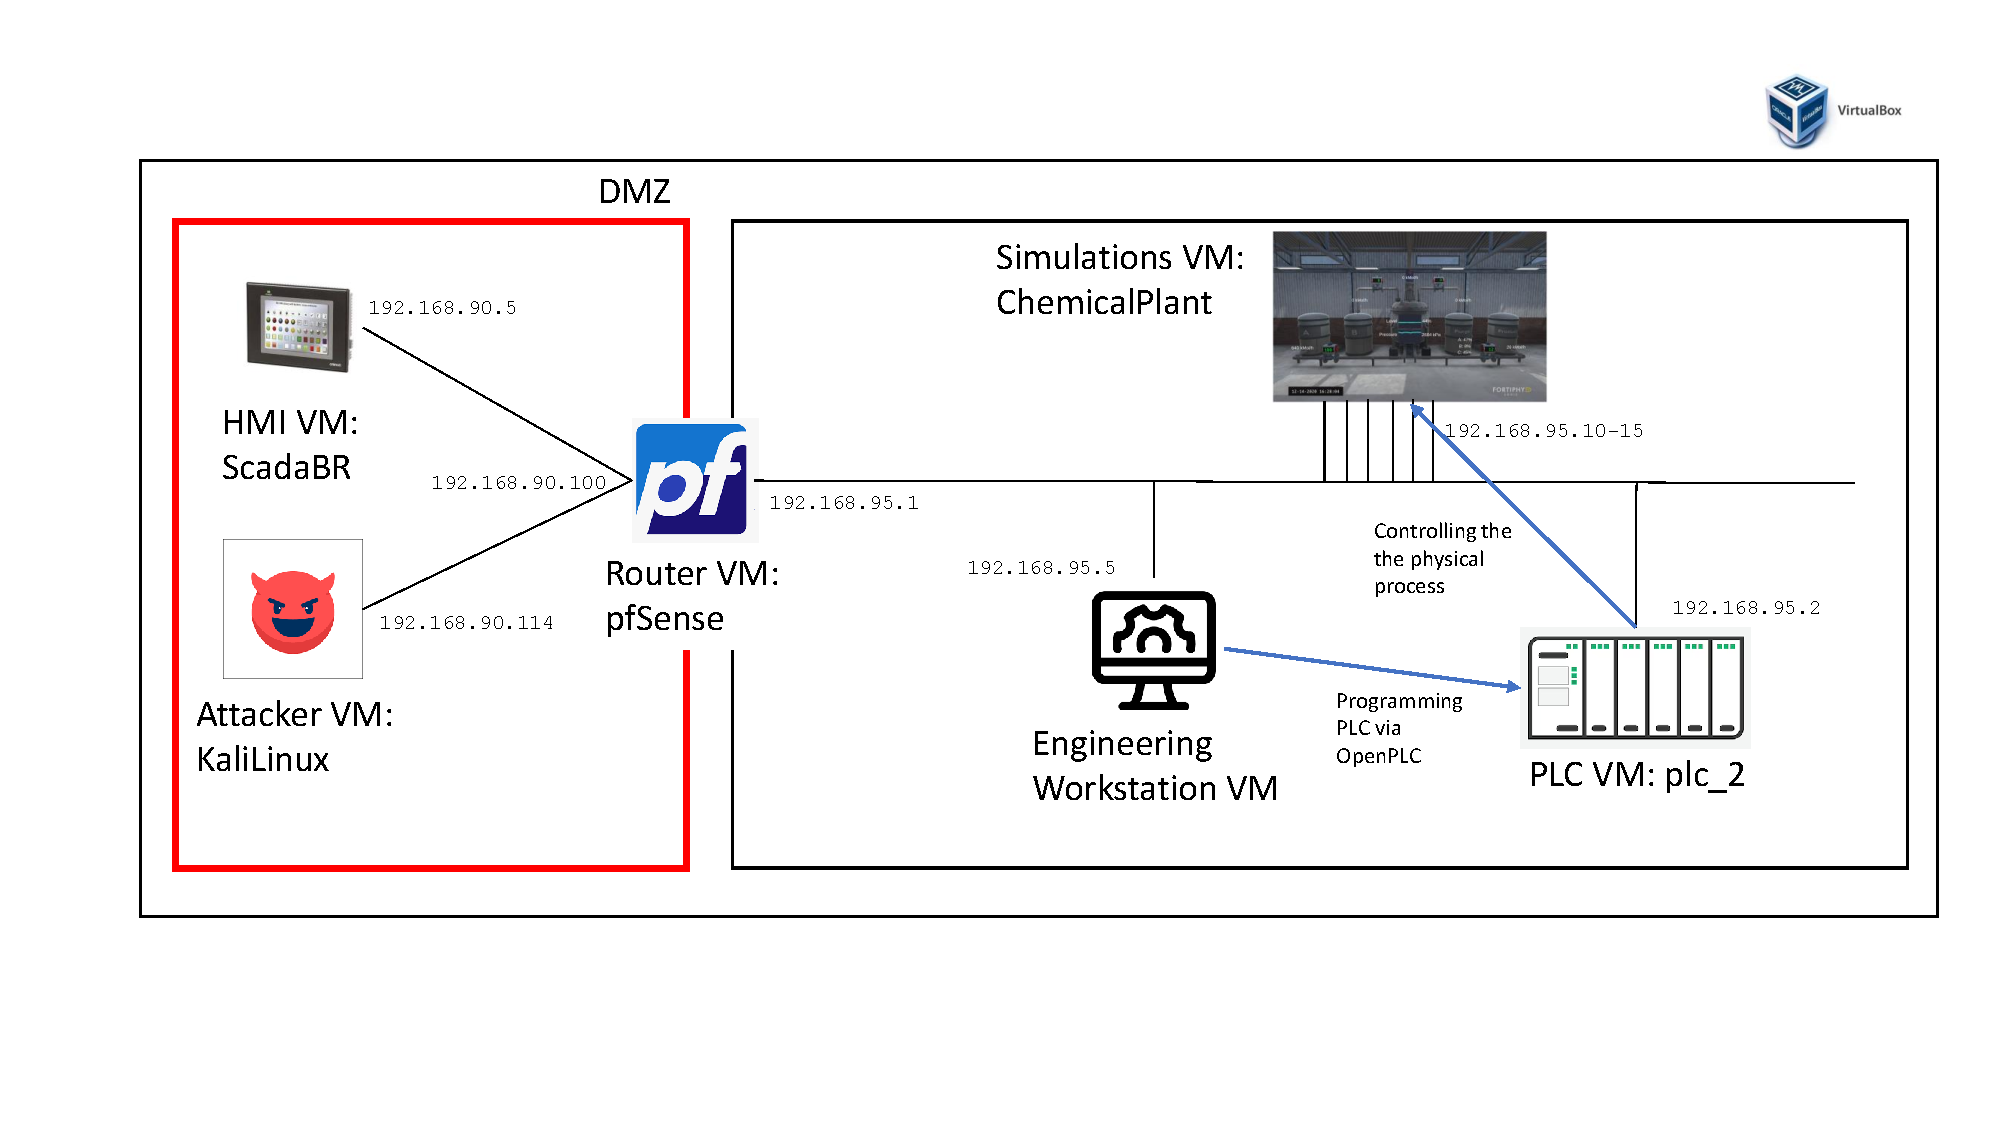
\includegraphics[width=\linewidth, trim={1cm 3cm 1cm 1cm}, clip]{figures/GRFICSv2_net_arch.pdf}
    \caption{Network architecture of the GRFICSv2. The GRFICSv2 makes use of six VMs (e.g, attacker, HMI, firewall, Engineering Workstation, PLC, and 3D process simulation) to model a cyberattack leading to an explosion of a chemical process.}
    \label{fig:GRFICSv2_arch}
\end{figure}

\chapter{Pressurized Water Reactor (PWR)}
\label{ch:pwr}
\begin{figure}[H]
    \centering
    \vspace{-1cm}
    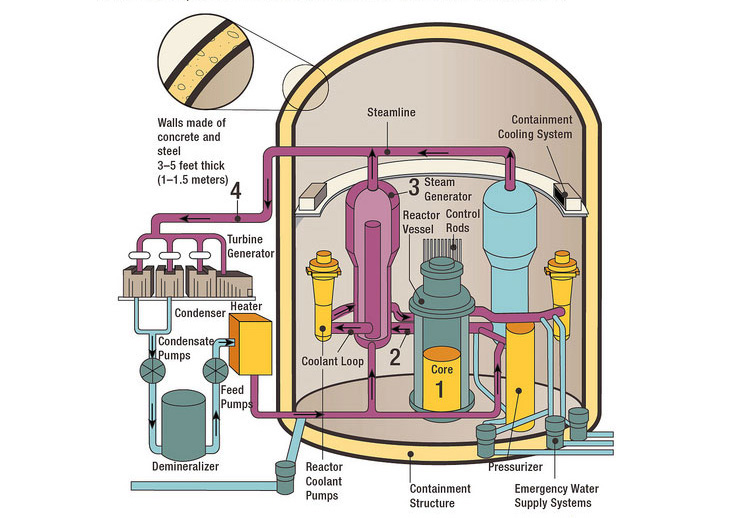
\includegraphics[width=\linewidth]{figures/pwr.jpg}
    \caption{Pressurized Water Reactor \cite{imgPwr}. 1. The core, situated in the reactor vessel, produces heat from nuclear reaction. 2. Pressurized water in the primary circuit carries the heat to the steam generator. 3. Inside the steam generator, heat from the primary circuit vaporizes the water in a secondary circuit, producing steam. The steam then rotates the rotor of the turbine generator, producing electromagnetic field variation which induces alternating current in the stator.}
    \label{fig:pwr}
    \hfill
\end{figure}
 
\chapter{Reactor Containment Building (CB)}
\label{ch:reactor_building}
\begin{figure}[H]
    \centering
    \vspace{-1cm}
    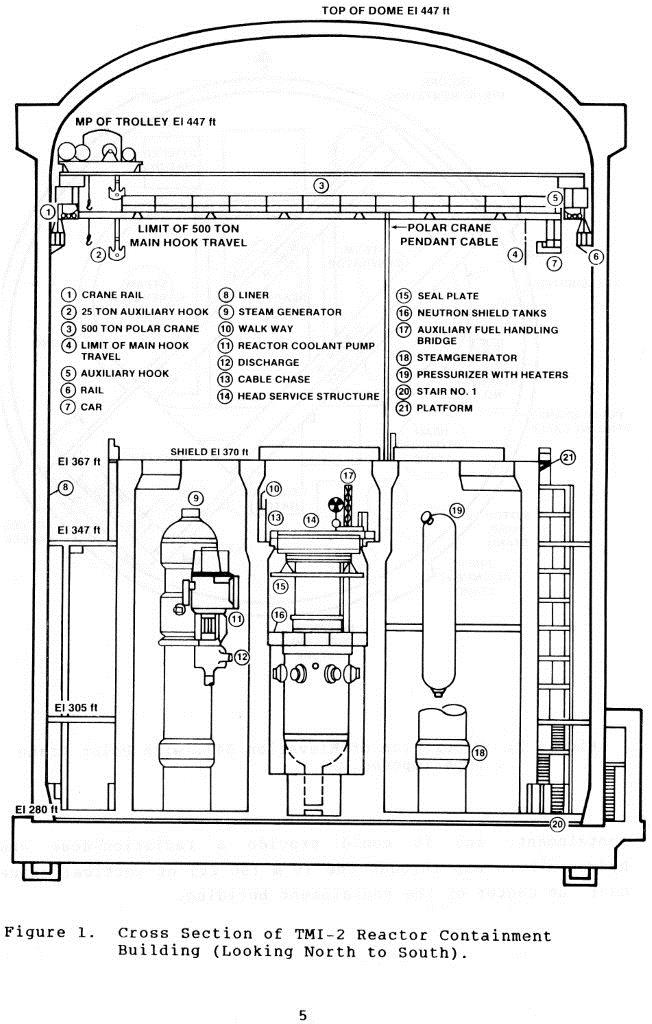
\includegraphics[width=0.5\linewidth]{figures/reactor_building.jpg}
    \caption{Reactor Containment Building (CB)~\cite{ONR-cs-br}. The Three Mile Island NPP CB is a 140 meters high and 80 cm thickness building that resists to internal accident situations (e.g., break of the primary circuit) and external aggressions (e.g., human origin or natural hazard).}
    \label{fig:reactor_building}
\end{figure}

\chapter{Purdue Model}
\begin{figure}[H]
    \centering
    \vspace{-0.75cm}
    \includegraphics[height=9cm]{figures/ICS-Purdue-Model.pdf}
    \caption{The Purdue Model: a Simplified Architecture of an ICS~\cite{imgPurdueModel}. The different levels an ICS architecture from Top to Bottom. 1. Level 5, in red, is the Corporate Network. This delocalized area is for example made of servers, or employees computer. 2. Level 4, in orange, is the Plant Network. It is mainly used for process reporting. 3. Level 3, in yellow, is the site control operations. It is separated with Level 4 by a DMZ that globally acts as a one-way firewall. The Level 3 is an area made for example of historians and process maintenance servers. The Level 2, in purple, is the SCADA. It is made of HMIs and allows technicians to visualize and supervise the process. The Level 1, in cyan, is the area process control it is mainly made of DCS (e.g., PLC, RTU or IIoT devices). The Level 0 is the process instrumentation made of actuators and sensors. As a side note, a polar crane's ICS is generally smaller and is an air-gap not connected to the Level 3 to 5.}
    \label{fig:purdue-model}
\end{figure}

\chapter{Threat Model}
\label{ch:threat_model}
\begin{figure}[H]
    \centering
    \vspace{-1.5cm}
    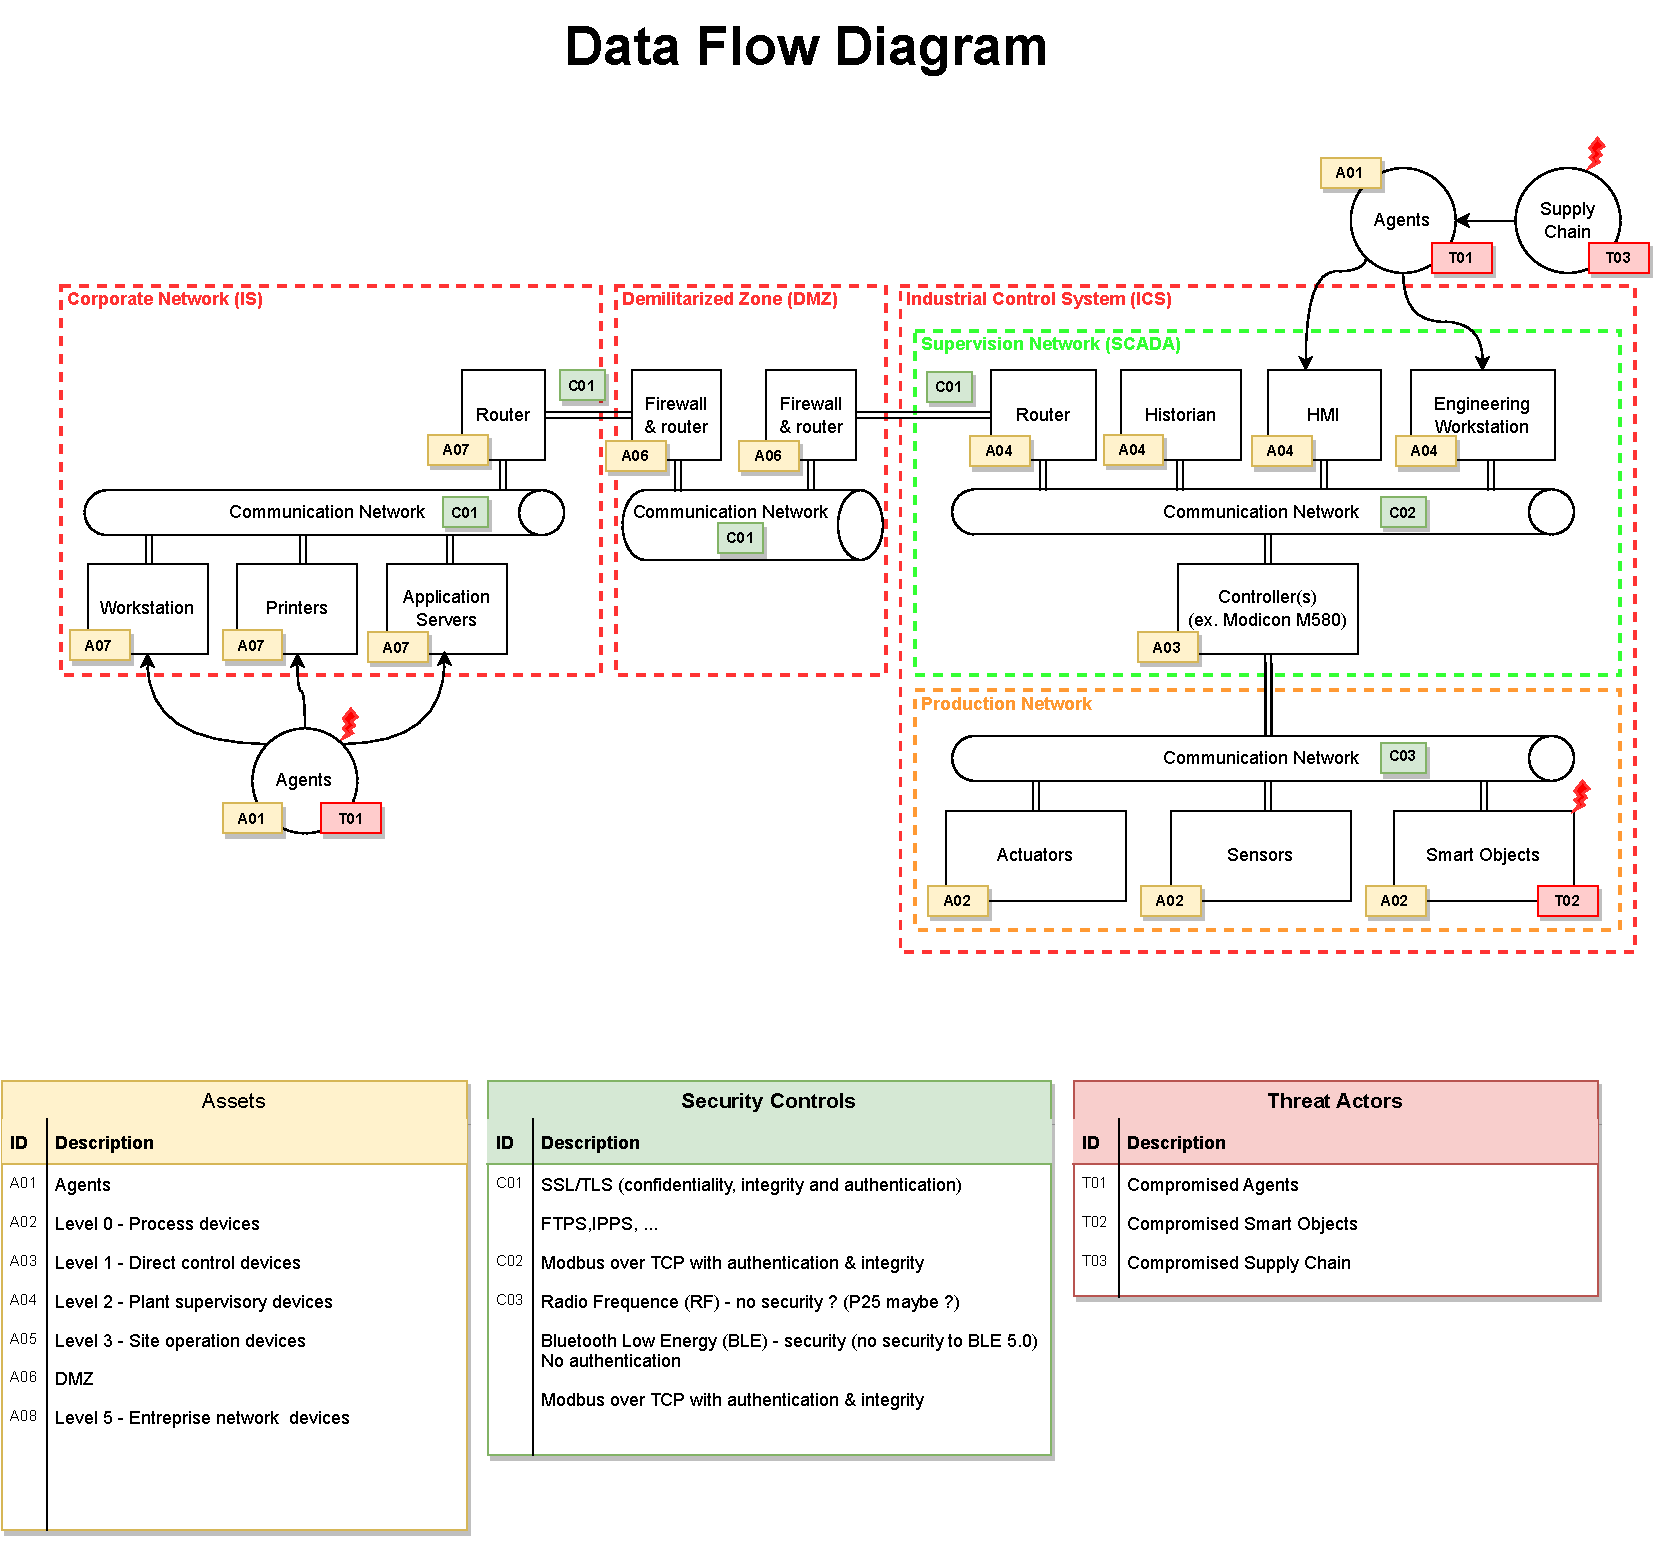
\includegraphics[height=12.7cm, angle=00, trim={0cm 0cm 0cm 2cm},clip]{figures/Threat-modelling-DFD.pdf}
    \caption{Data flow diagram. From an ICS architecture, this data flow diagram represents the three entry points identified – the corporate network, the supervision network, or the production network. The \emph{NinjaCrane} attack infects first the supervision network via a malicious HID USB to then tamper the production network.}
    \label{fig:data_flow_diagram}
\end{figure}

\begin{figure}
    \centering
    \vspace{2cm}
    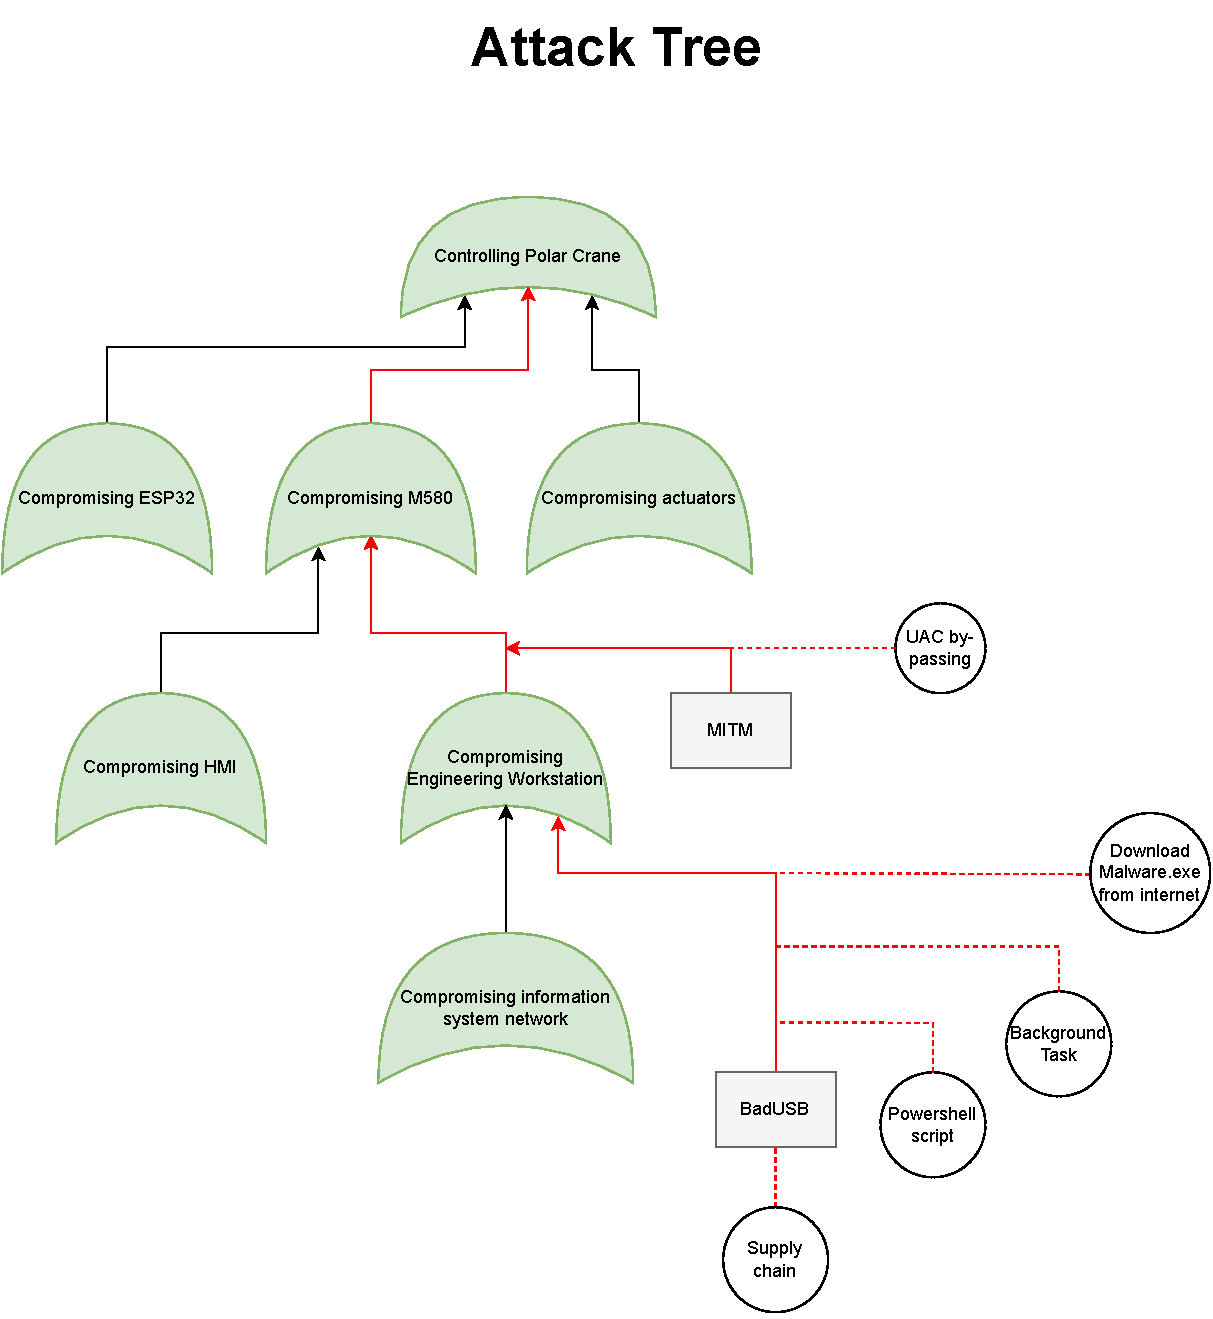
\includegraphics[height=12cm, angle=90, trim={0cm 0cm 0cm 2cm},clip]{figures/Threat-modelling-Attack Tree.pdf}
    \caption{Attack tree. The attack tree models the path taken to take control over the polar crane. The first step is the supply chain compromising that brings a HID-capable device to be connected to the engineering workstation. When connected, the USB device runs a powershell script to download and execute in background a malware. This malware by-pass the windows UAC and performs a MITM attack to modify PLC's internal variables and take control over the polar crane.}
    \label{fig:atk-tree}
\end{figure}

\chapter{Polar Crane's Testbed}

\begin{figure}[H]
    \centering
    \vspace{-1.3cm}
    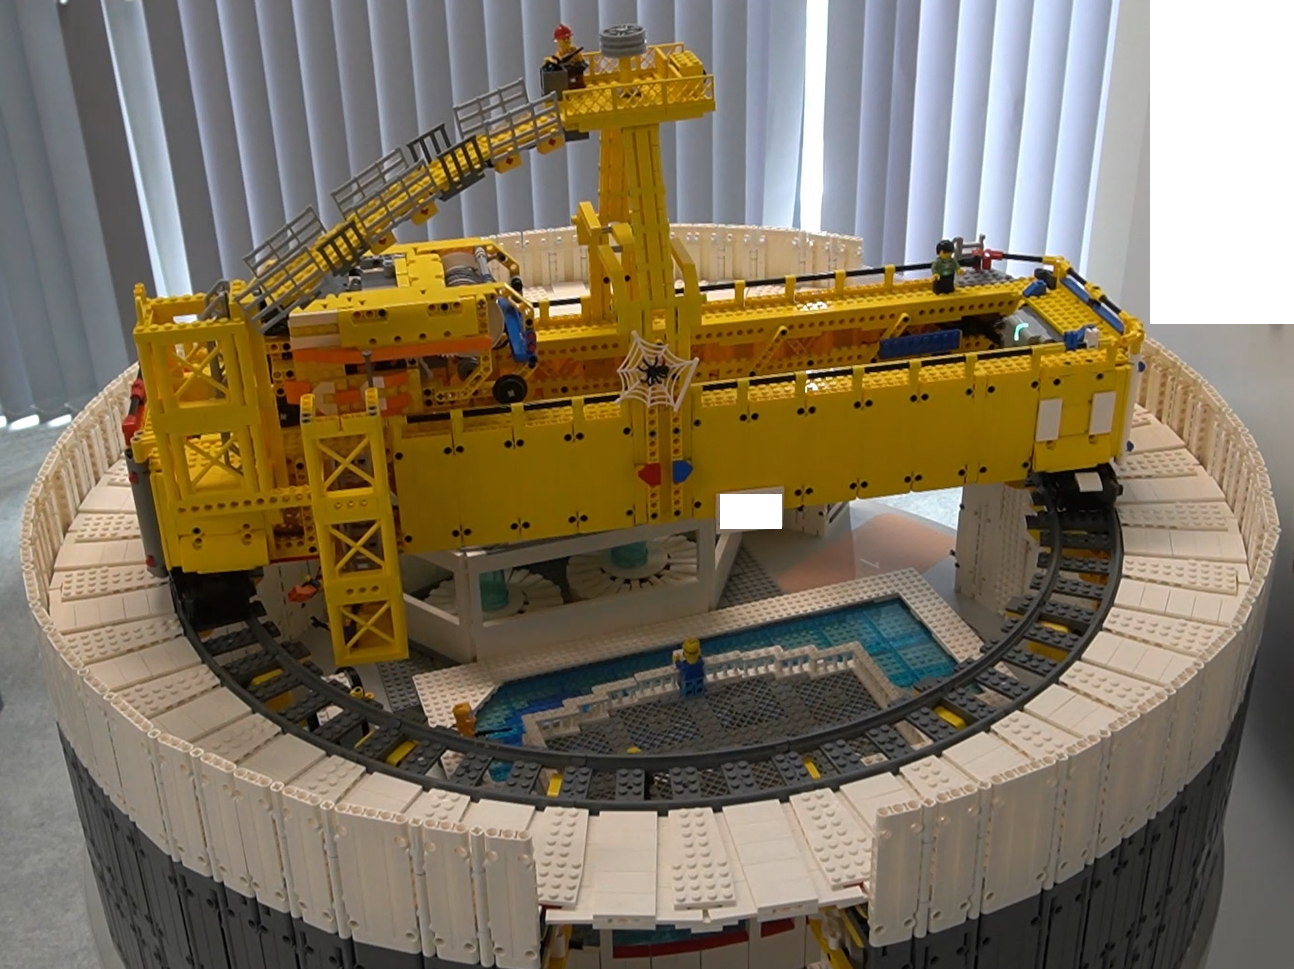
\includegraphics[width=\linewidth]{figures/polar-crane}
    \caption{Polar Crane's Sketch. Sketch in LEGO\texttrademark of the polar crane which models three different movements; crane rotation, trolley rectilinear displacement, and charge lift. Those movements are controlled via an HMI connected to the \emph{Modicon M580} PLC. The PLC interprets and transmits the commands to three LEGO\texttrademark BLE Hubs via an ESP32 microcontroller establishing the Bluetooth connection.}
    \label{fig:polar-crane}
\end{figure}

\begin{figure}
    \centering
    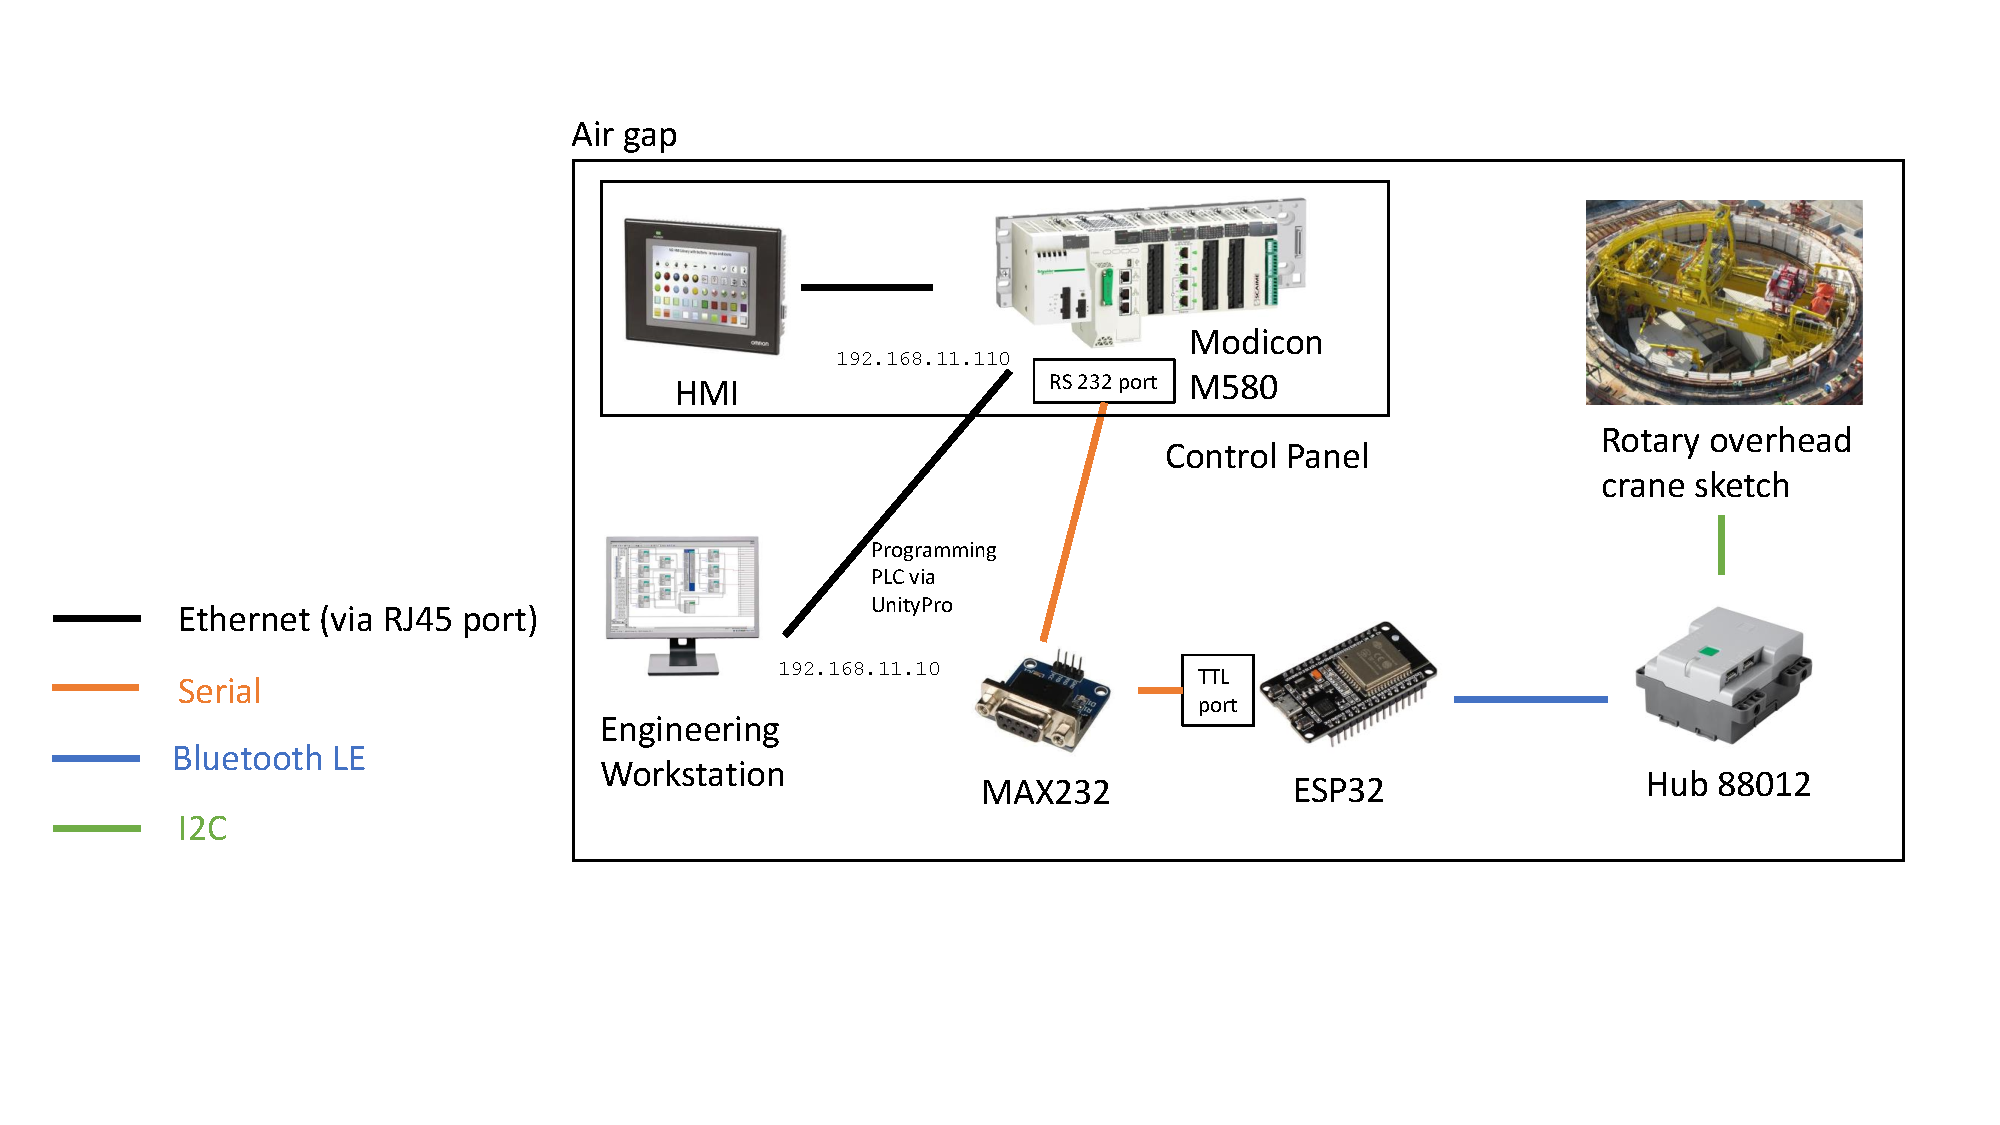
\includegraphics[width=\linewidth]{figures/Setup.pdf}
    \caption{Network Architecture of the Testbed. The Engineering Workstation programs the M580 PLC via Unity Pro. The M580 stores and executes the polar crane's program. The HMI displays the state (i.e., position, speed etc.) of the polar crane and allows a technician operator to control the polar crane. Due to its rotation, the polar crane must be controlled over the air. In this testbed the choice has been made to control the polar crane with BLE. The ESP32 is sending over BLE the commands it received from the PLC.}
    \label{fig:setup}
\end{figure}

\chapter{Malicious Mouse}
\begin{figure}[H]
    \centering
    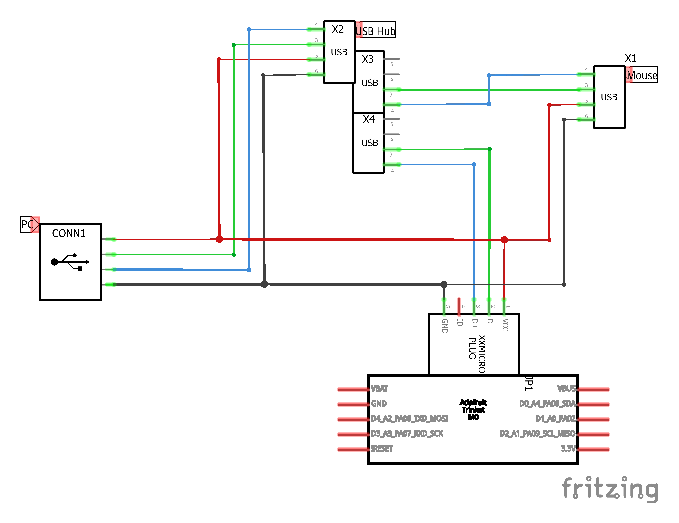
\includegraphics[height=9cm, angle=90, trim={0cm 0cm 0cm 0cm},clip]{figures/Sketch_wired_mouse_basUSB.pdf}
    \caption{Electric wired schematic of the malicious mouse. The mouse connection originates from the  \texttt{CONN1} (e.g., PC USB connection) and proceeds to an USB hub that splits the connection into two pathways – one leading to the mouse itself and the other one to an HID-capable microcontroller.}
    \label{fig:infected-mouse-wiring}
\end{figure}

\begin{figure}
    \centering
    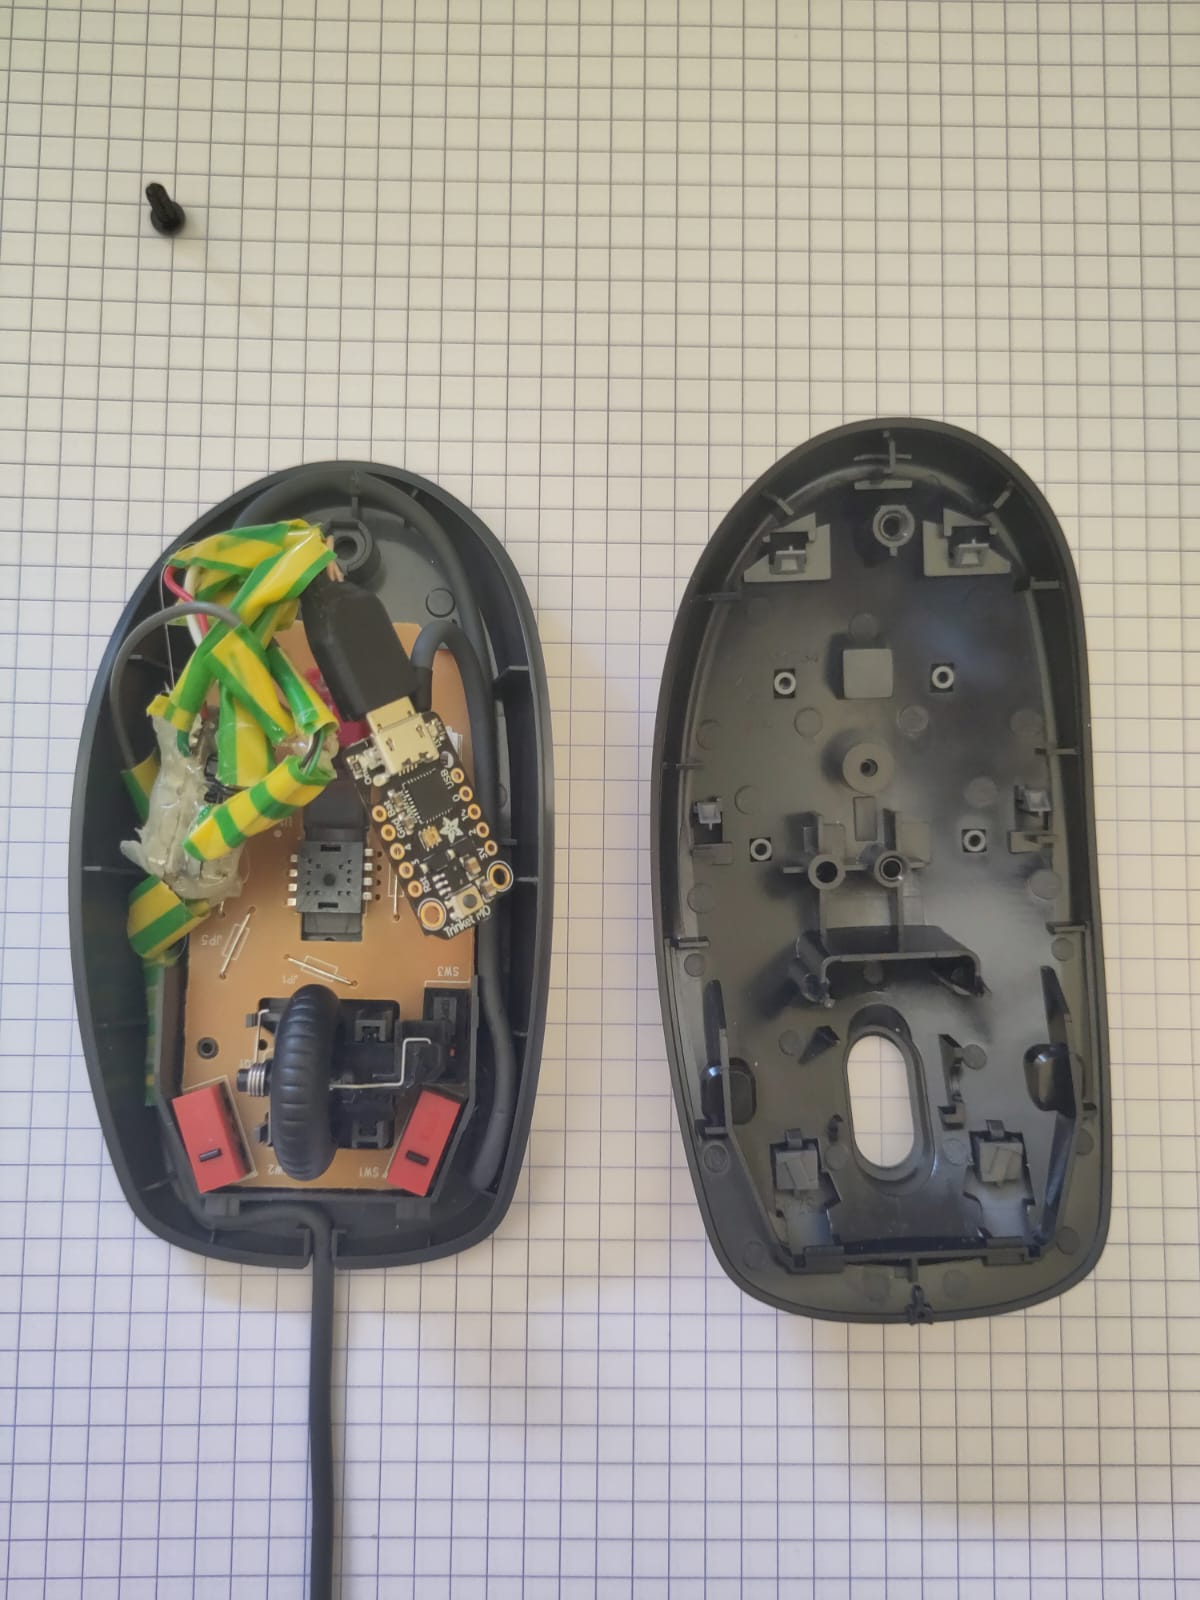
\includegraphics[height=13cm, trim={0cm 5cm 0cm 5cm},clip]{figures/infected-mouse.jpeg}
    \caption{Picture of the maliciously modified mouse. A Logitech mouse opened and modified in order to include an HID-capable microcontroller. On the photograph can be seen the Adafruit Trinket M0 connected in micro-USB to the hub.}
    \label{fig:infected-mouse-photo}
\end{figure}

\chapter{Modbus/UMAS Communication}
\begin{figure}[H]
    \centering
    \vspace{-0.5cm}
    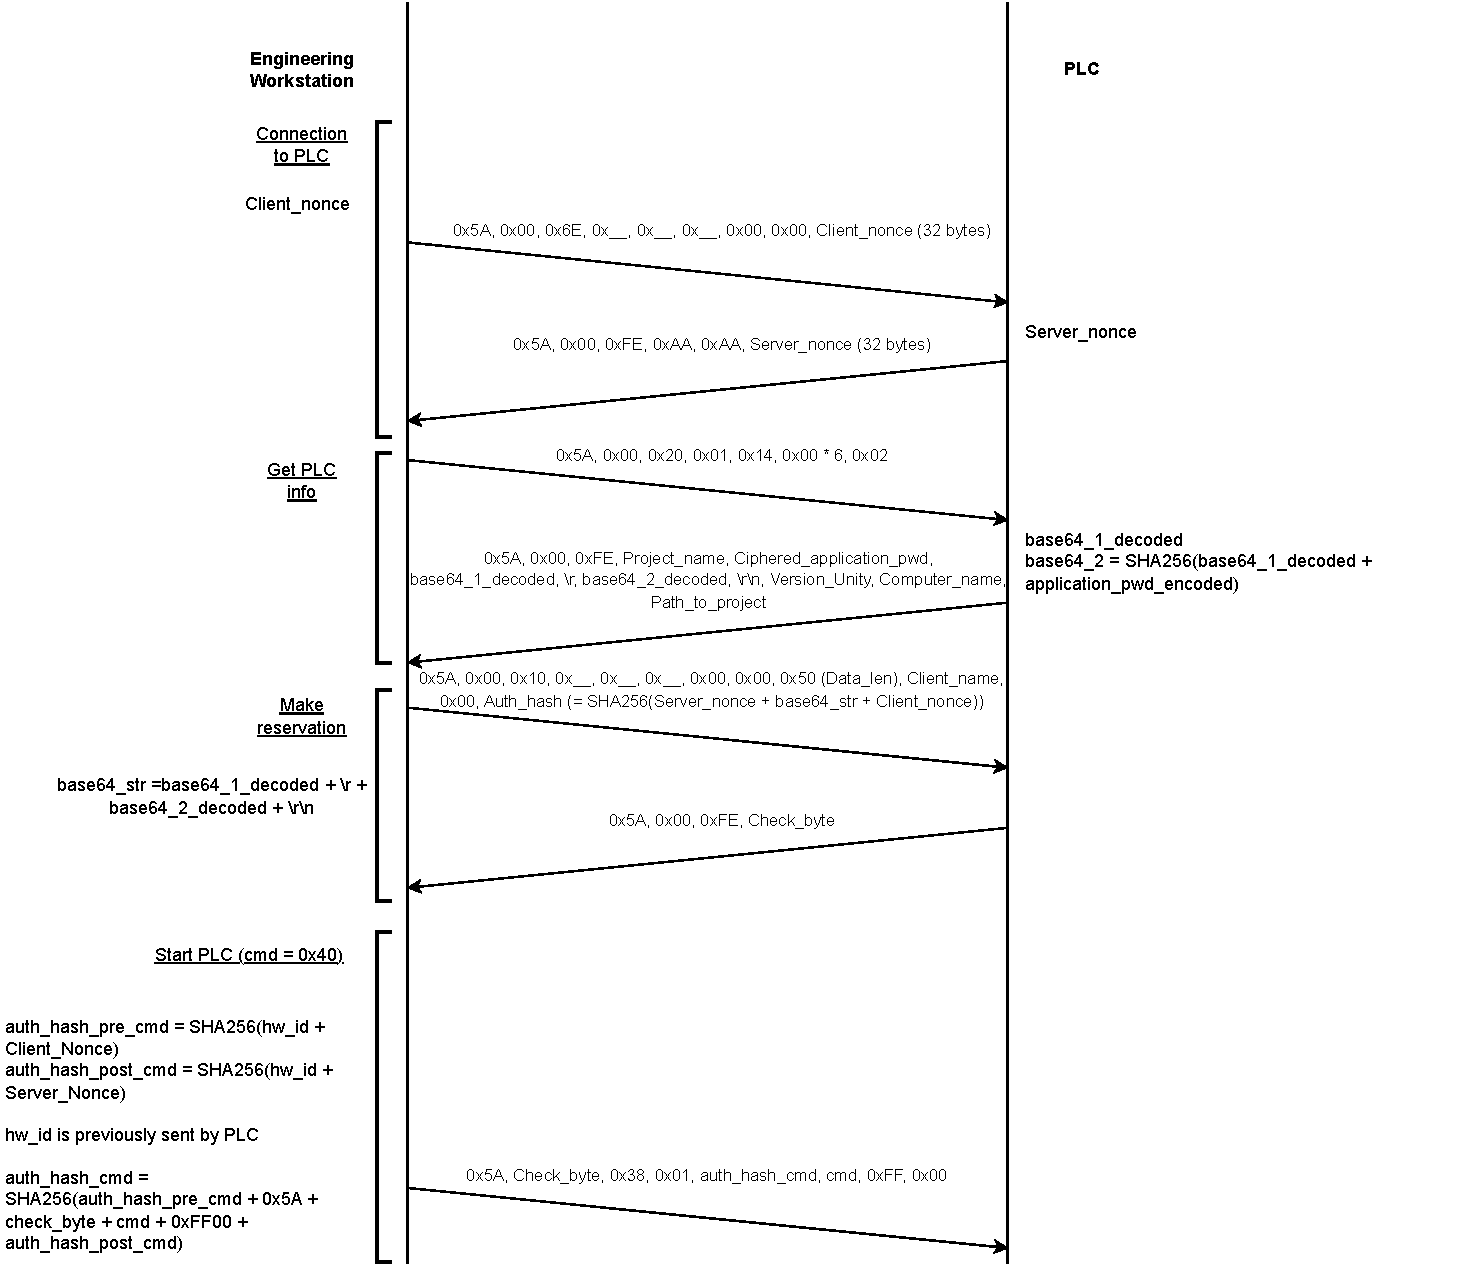
\includegraphics[width=0.95\linewidth]{figures/ModiPwn-Page-1.pdf}
    \caption{Communication between the M580 and the engineering workstation}
    \label{fig:communication}
\end{figure}

\chapter{Adversary's Graphical User Interface (GUI)}
\begin{figure}[H]
    \centering
    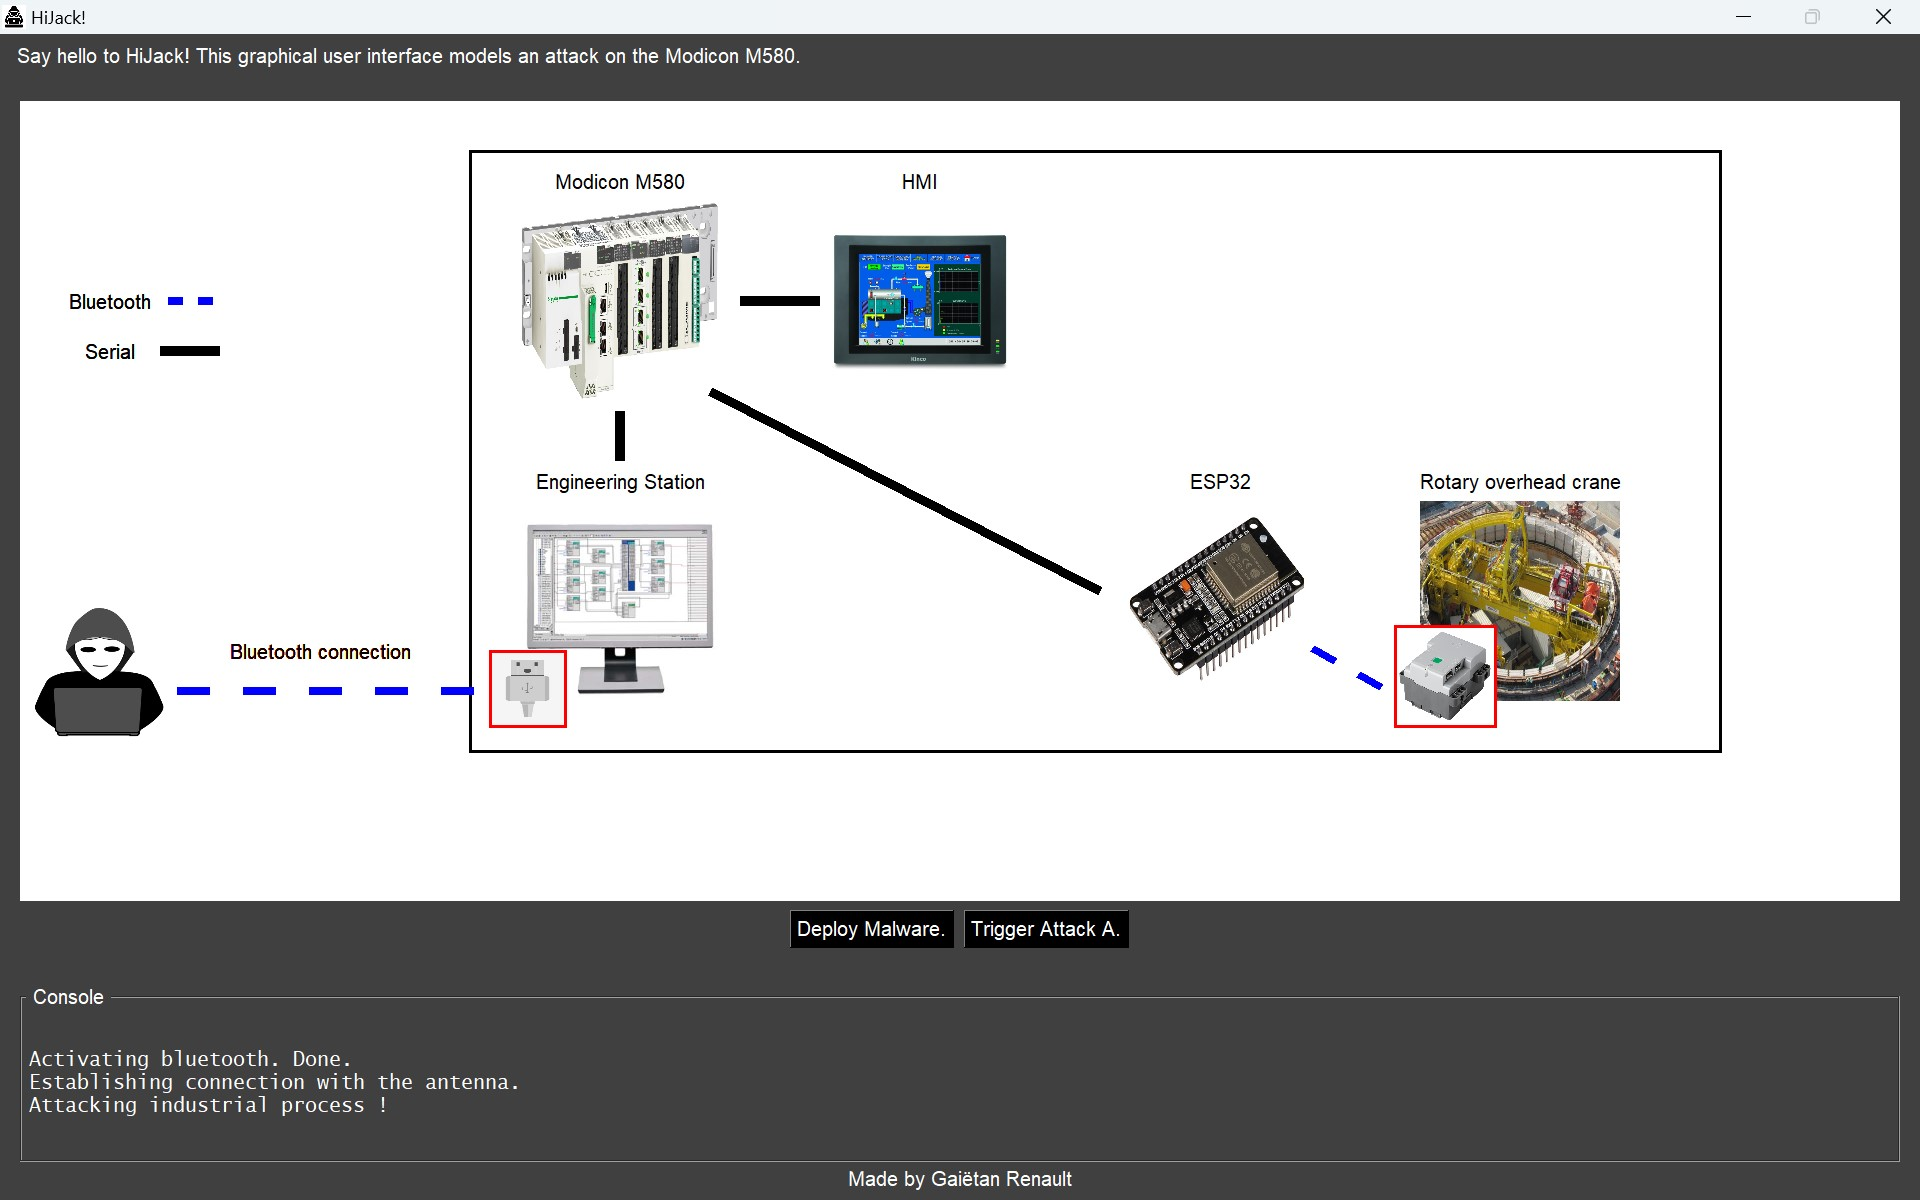
\includegraphics[width=\linewidth, angle=00, trim={0cm 0cm 0cm 0cm},clip]{figures/GUI.jpg}
    \caption{Adversary's Graphical User Interface (GUI). This interface, running on a laptop, is made with \href{https://www.pysimplegui.org/en/latest/}{\emph{PySimpleGUI}} and allows to take control of the USB Ninja cable over BLE by triggering two different payloads. The first one deploys the malware on the PC, the second one starts the \emph{NinjaCrane} attack.}
    \label{fig:gui}
\end{figure}

\chapter{Data Exfiltration}
\begin{figure}[H]
    \centering
    \vspace{-0.5cm}
    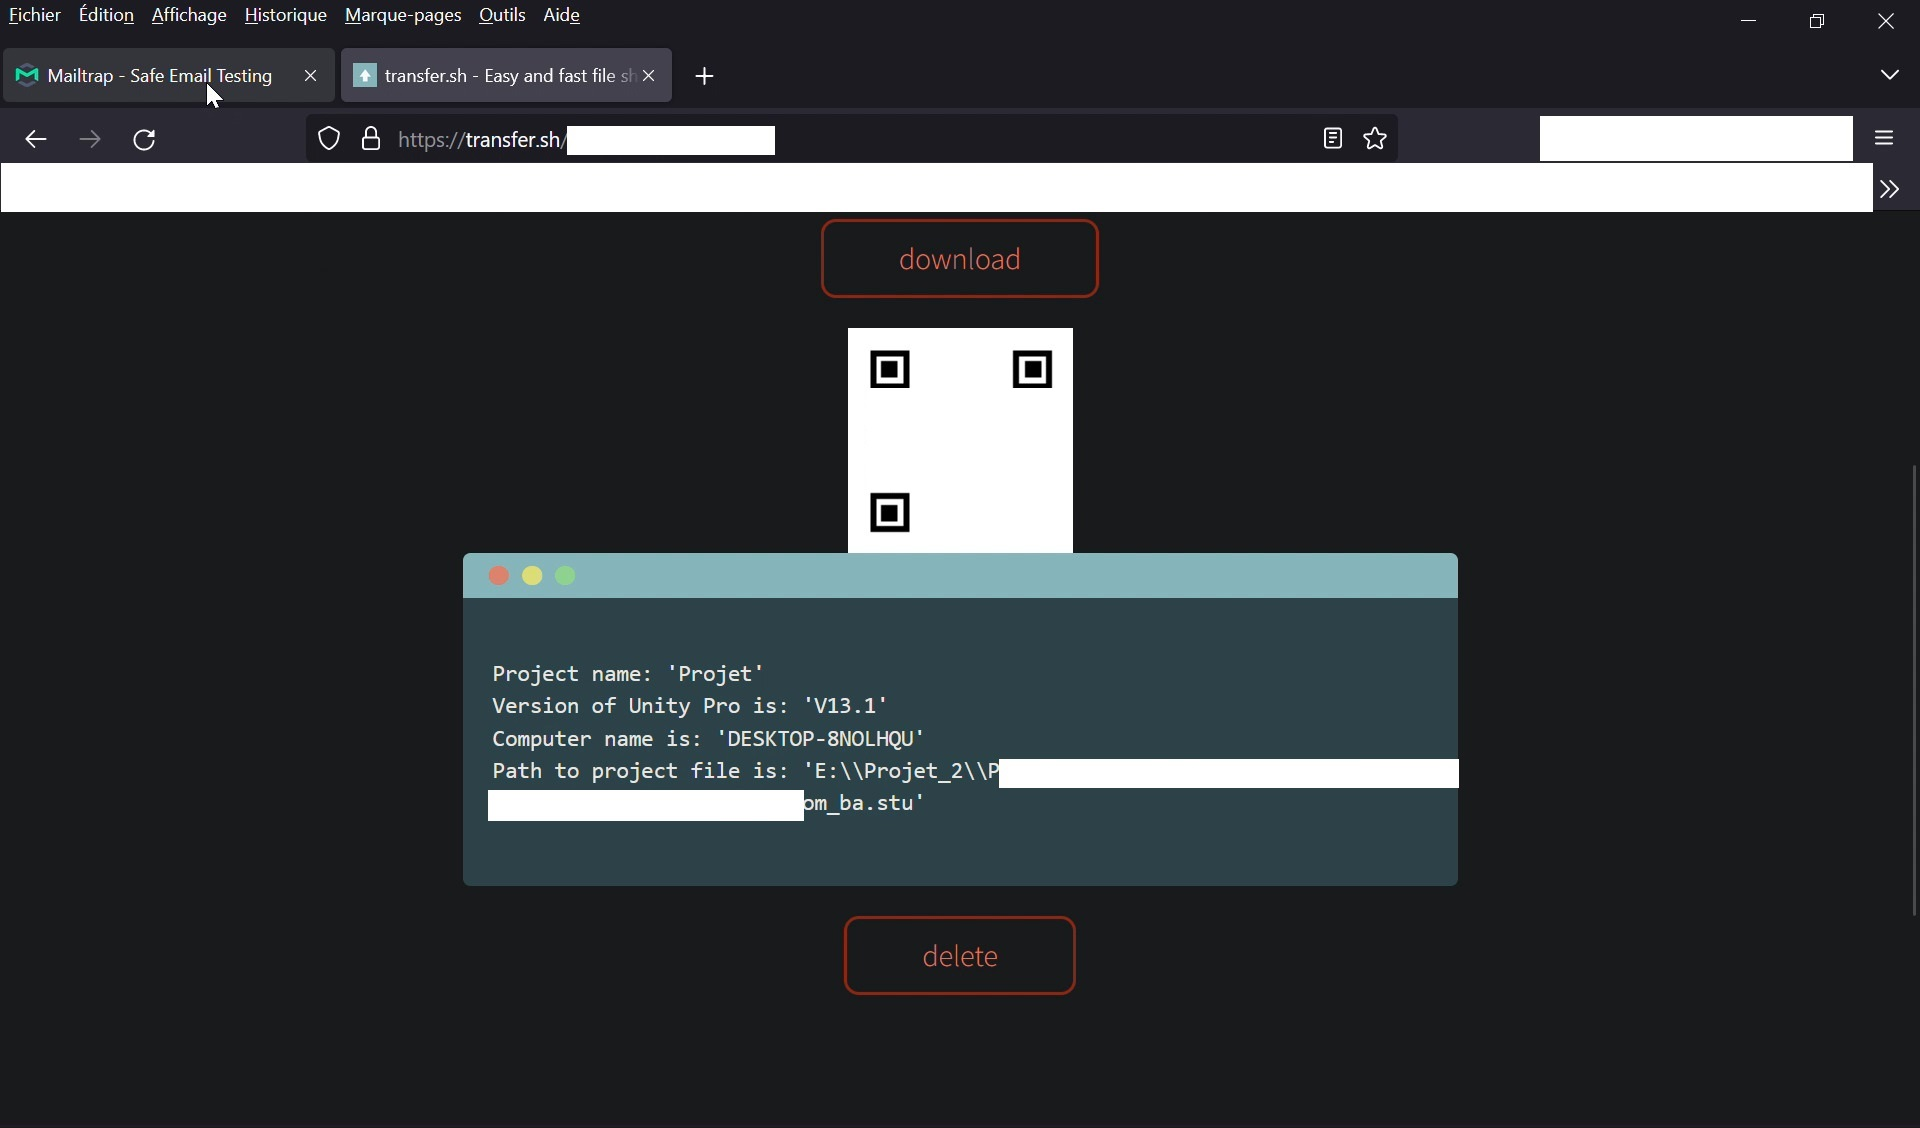
\includegraphics[width=0.7\linewidth]{figures/mailtrap-project-infos.jpg}
    \\ \vspace{0.5cm}
    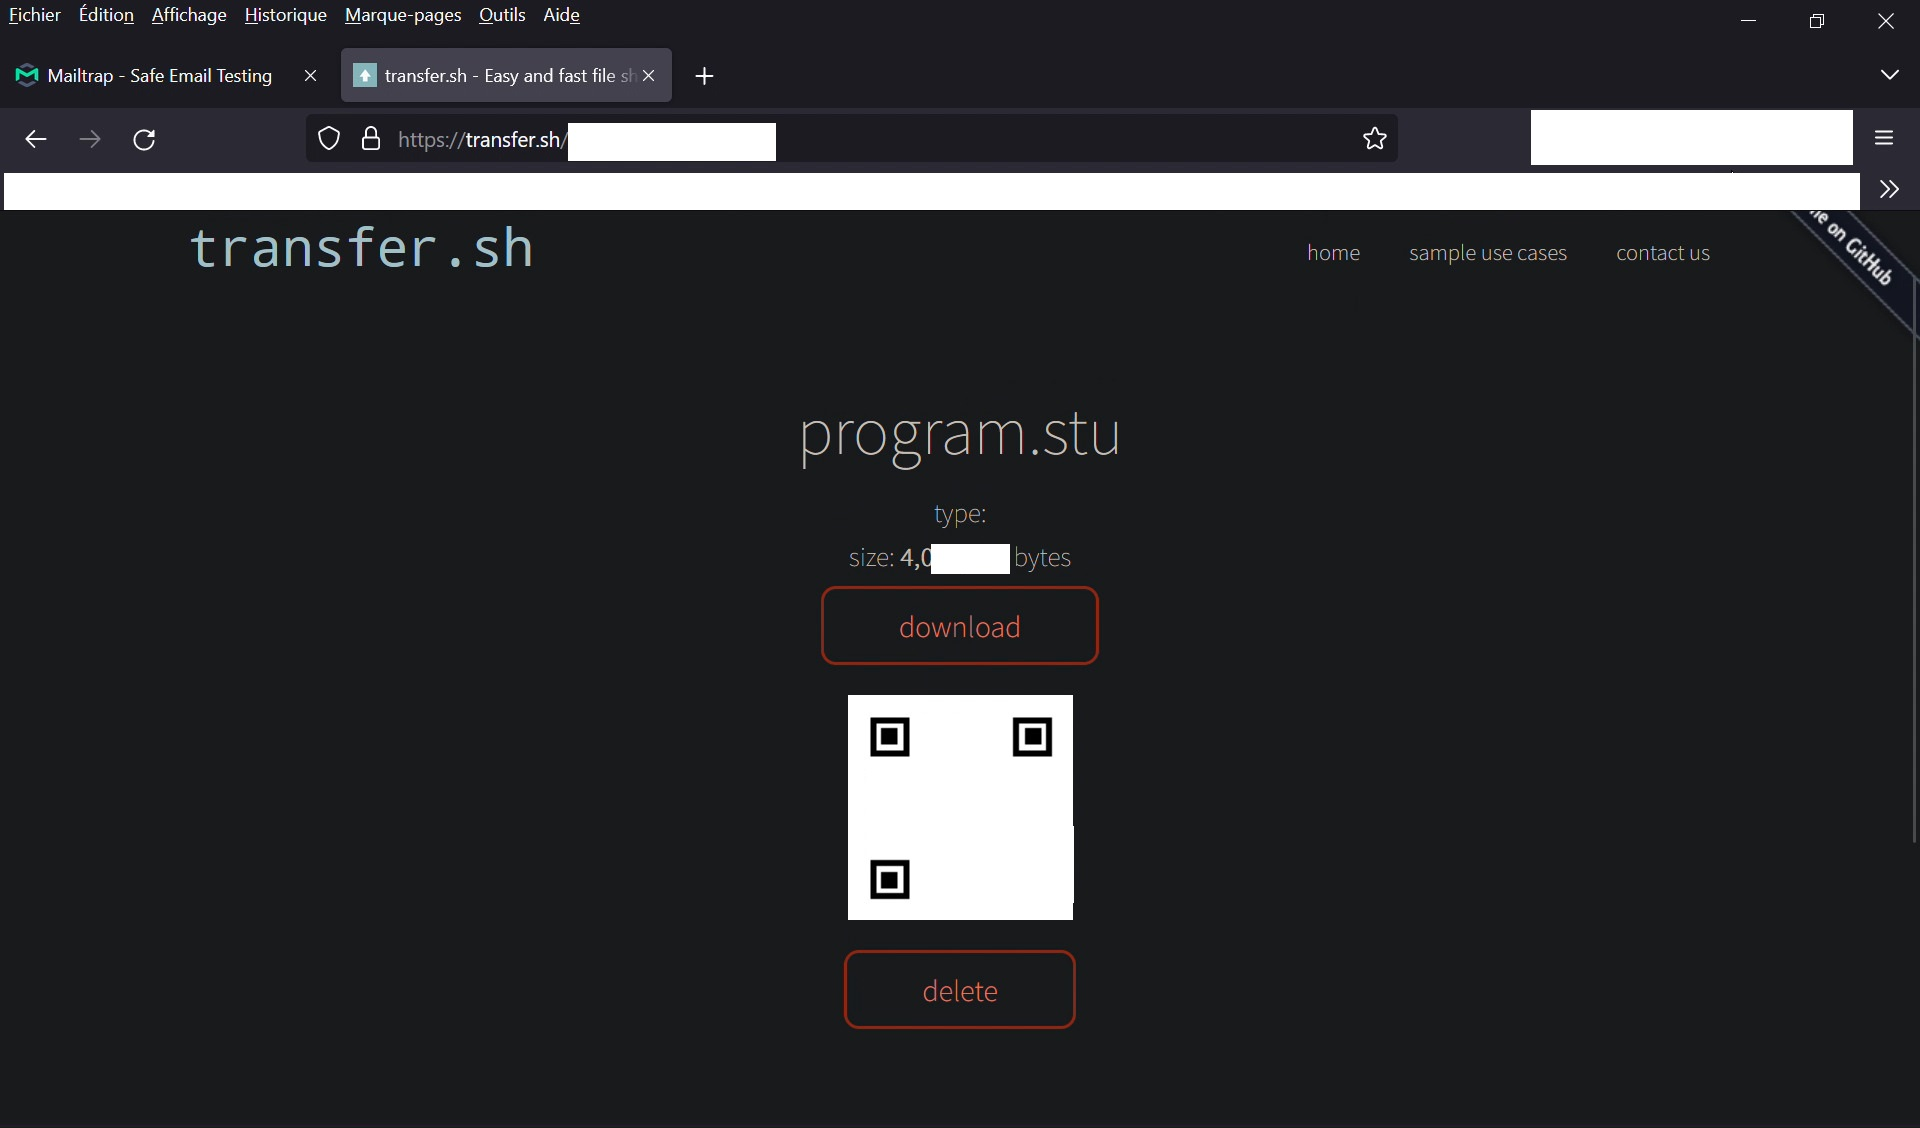
\includegraphics[width=0.7\linewidth]{figures/mailtrap-stu.jpg}
    \caption{Data exfiltration over internet. Top: Project information. Bottom: .STU program.}
    \label{fig:mailtrap-exfiltrate-data}
\end{figure}

\chapter{HID-device's Flowchart Payload}
\begin{figure}[H]
    \centering
    \vspace{-1cm}
    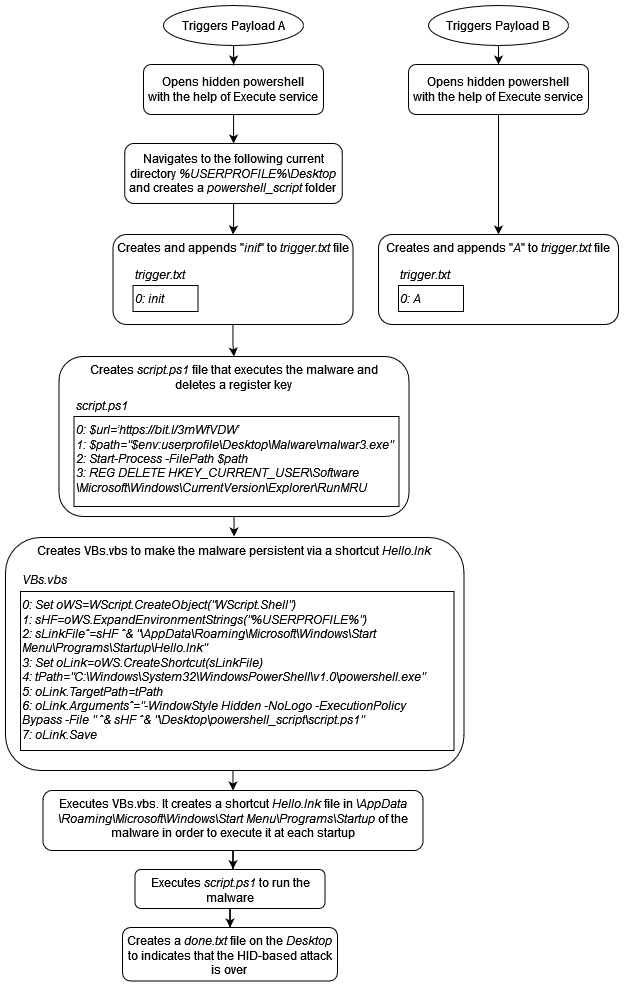
\includegraphics[height=13cm, angle=0, trim={0cm 0cm 0cm 0cm},clip]{figures/logigramme.png}
    \caption{HID-device's flowchart payload.}
    \label{fig:logigram}
\end{figure}

\chapter{Live Demonstration Feedback from the Participants}
\label{annex:feedback}

\begin{itemize}
    \item « The cyberattack of the polar crane was extremely well realised because it was very assiduous and very practical: we directly observe how a human-origin mistake (USB cable plug-in) could have consequences on a NPP site. »
    \item « Cybersecurity workshop was interesting and playful. »
    \item « Cybersecurity workshop was very interesting. Congrats to the job done for preparing it, it was immersive and great. »
    \item « Cybersecurity, very good in form and content, it's an eye-opener on the importance of ensuring safety. »
    \item « Cybersecurity: Discovering new dangers for nuclear facilities. Complexity of protecting against this type of risk, given the development of new technologies (AI in particular). »
    \item « Cyber-crime: Excellent! A return to childhood via the lego sketch, which can be moved and even controlled by the PLC. The workshop on cyber-security really made us realize that evil can lurk anywhere... very instructive! »
    \item « Polar crane hacking: very good, very entertaining, with visual elements. The trainee presented extremely well (very good popularization for non-experts), [...]. I'd perhaps recommend a longer workshop (to allow more questions) and with fewer people, to allow people to move around the polar crane demo and the engineering workstation. »
\end{itemize}


% %%%%%%%%%%%%%%%%%%%%%%%%%%%%%%%%%%%%%%
%
% In case you ever need an (optional) appendix.
%
% You need the following items:
% \begin{itemize}
% \item A box
% \item Crayons
% \item A self-aware 5-year old
% \end{itemize}

\end{document}